% !TEX TS-program = pdflatex

\documentclass[12pt,a4paper, twoside]{article}
\usepackage[utf8]{inputenc}
\usepackage[german]{babel}
\usepackage[inner=3cm,outer=2cm,top=2cm,bottom=2cm]{geometry}
\usepackage{amsmath}
\usepackage{setspace}
\usepackage{arydshln}
\usepackage{array}
\setlength\extrarowheight{5pt}
\usepackage{multicol}
\usepackage{textcomp}
\usepackage{amsthm}
\usepackage{microtype}
\usepackage{booktabs}
\usepackage{etoolbox}
\usepackage{makecell}
\usepackage{hyperref}
\usepackage{framed}
\usepackage{chemmacros}
\usepackage{bbold}
\usepackage{mathrsfs}
\usepackage{amssymb}
\usepackage{graphicx}
\usepackage{tikz}
\usepackage[bottom]{footmisc}
\usetikzlibrary{arrows}
\usepackage{tikz-3dplot}
\usepackage{cancel}
\usepackage{wrapfig}
\DeclareMathOperator{\tr}{tr}
\usepackage{esint}
\usepackage{multicol}
\usepackage{tabularx}
\hypersetup{
    colorlinks,
    citecolor=black,
    filecolor=black,
    linkcolor=black,
    urlcolor=black
}
\let\vaccent=\v
\renewcommand{\v}[1]{\ensuremath{\mathbf{#1}}}
\newcommand{\iu}{{i\mkern1mu}}
\newcommand{\gv}[1]{\ensuremath{\mbox{\boldmath$ #1 $}}}
\newcommand{\abs}[1]{\left| #1 \right|}
\newcommand{\avg}[1]{\left< #1 \right>}
\let\underdot=\d
\renewcommand{\d}[2]{\frac{d #1}{d #2}}
\newcommand{\dd}[2]{\frac{d^2 #1}{d #2^2}}
\newcommand{\pd}[2]{\frac{\partial #1}{\partial #2}}
\newcommand{\pdd}[2]{\frac{\partial^2 #1}{\partial #2^2}}
\newcommand{\pdc}[3]{\left( \frac{\partial #1}{\partial #2}
 \right)_{#3}}
\newcommand{\ket}[1]{\left| #1 \right>}
\newcommand{\bra}[1]{\left< #1 \right|}
\newcommand{\braket}[2]{\left< #1 \vphantom{#2} \right|
 \left. #2 \vphantom{#1} \right>}
\newcommand{\matrixel}[3]{\left< #1 \vphantom{#2#3} \right|
 #2 \left| #3 \vphantom{#1#2} \right>}
\newcommand{\grad}[1]{\nabla #1}
\let\divsymb=\div
\renewcommand{\div}[1]{\nabla \cdot #1}
\newcommand{\rot}[1]{\nabla \times #1}
\let\baraccent=\=
\renewcommand{\=}[1]{\stackrel{#1}{=}}
\def\dbar{{\mathchar'26\mkern-12mu d}}
\newcommand{\rd}{\abs{\vec r - \vec r'}}
\newcommand{\ort}{\vec r}
\newcommand{\js}{\vec \jmath}
\newcommand{\erw}[1]{\langle #1 \rangle}
\newcommand{\eps}{\varepsilon}
\newcommand{\units}[2]{\frac{\text #1}{\text #2}}


\def\dbar{{\mathchar'26\mkern-12mu d}}
\newtheorem{satz}{Satz}
\theoremstyle{definition}
\newtheorem{dfn}{Definition}
\theoremstyle{remark}
\newtheorem*{rmk}{Bemerkung}
\thispagestyle{empty}
\title{Enchiridion Physic\ae}
\author{Andreas Hemmetter}

\definecolor{white}{RGB}{255,255,255}
\definecolor{darkgray}{HTML}{333333}
\definecolor{gray}{HTML}{4D4D4D}
\definecolor{lightgray}{HTML}{999999}
\definecolor{verylightgray}{HTML}{EEEEEE}
\definecolor{green}{HTML}{39AF5D}
\definecolor{orange}{HTML}{FDA333}
\definecolor{purple}{HTML}{D3A4F9}
\definecolor{red}{HTML}{FB4485}
\definecolor{blue}{HTML}{6CE0F1}

% for the notes, remarks and definitions at the beginning of a subsection
\newcommand{\notes}[1]{%
\textit{#1}\\
\hrule
}

% for the layout of a concept with conditions
\newcommand{\conceptcon}[3]{%
\noindent
\begin{framed}
\noindent\textbf{#1} \\
\textit{#2}
\par\begin{tabular}{p{0.9\linewidth}}
#3
\end{tabular}
\end{framed}
}

% for the layout of a concept
\newcommand{\concept}[2]{%
\noindent
\begin{framed}
\noindent\textbf{#1}
\par\begin{tabular}{p{0.9\linewidth}}
#2
\end{tabular}
\end{framed}
}

% for one entry with additional explanation in a concept environment
\newcommand{\fnote}[3]{%
\noindent\begin{tabularx}{\linewidth}{@{}p{5cm}X}
#1 & $#2$\\
& \textit{\small{#3}}
\end{tabularx}}

% for an entry without explanation, just a formula and its name
\newcommand{\f}[2]{%
\noindent\begin{tabularx}{\linewidth}{@{}p{5cm}X}
#1 & $#2$
\end{tabularx}}

\newcommand{\img}[1]{%
\includegraphics[height=4cm]{pic/#1}
}

\BeforeBeginEnvironment{framed}{\begin{minipage}{\linewidth}}
\AfterEndEnvironment{framed}{\end{minipage}\par}


\makeatletter
\def\@maketitle{

\begin{center}
{\Huge \bfseries \sffamily \@title }\\[20ex]
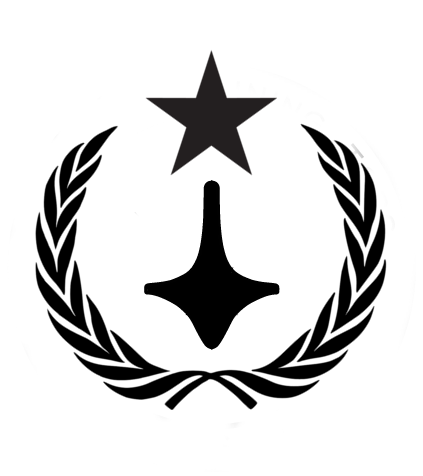
\includegraphics[width = 80mm]{pic/logofah.png}\\
\vfill
{\Large  \@author}\\[5ex]
Aachen, \@date
\end{center}}
\makeatother

\begin{document}

\maketitle
\thispagestyle{empty}
\newpage

\begin{multicols}{2}
\tableofcontents
\end{multicols}


\newpage
\setstretch{1.5}





\section{Mechanik}

\subsection[Kinematik des Massenpunktes]{Kinematik des Massenpunktes\let\thefootnote\relax\footnote{$g$: Fallbeschleunigung $[\frac{m}{s^2}]$, $c_W$: Luftreibungskoeffizient, $D$: Direktionsmoment $[Nm]$, $q$: elektrische Ladung $[C]$, $E$: elektrisches Feld $[\frac{V}{m}]$, $B$: magnetische Flussdichte $[Am]$, $\varepsilon_0$: elektrische Feldkonstante $[\frac{As}{Vm}]$}}

\notes{Ein Massenpunkt hat keine Ausdehnung und reagiert auf Kräfte genau an einem Punkt. Daher können Drehungen des Punktes nicht definiert werden.}

\conceptcon{Schiefer Wurf}{homogenes Gravitationsfeld ohne Luftwiderstand}{
\f{Bewegungsgleichung}{y(x) = - \frac{g}{2 v_0^2 \cdot \cos^2(\alpha)} x^2 + \tan(\alpha) x + y_0}\\
\f{Steigzeit}{T_s = \frac{v_0}{g} \sin(\alpha)}\\
\f{Wurfhöhe}{h = \frac{v_0^2}{2g} \sin^2(\alpha)}\\
\f{Wurfweite}{R = \frac{v_0^2}{g} \sin^2(\alpha)}
\fnote{Abwurfwinkel}{\alpha_{max} = \arcsin \frac{v_0}{\sqrt{2 v_0^2 + 2 g y_0}}}{für maximale Wurfweite}
}

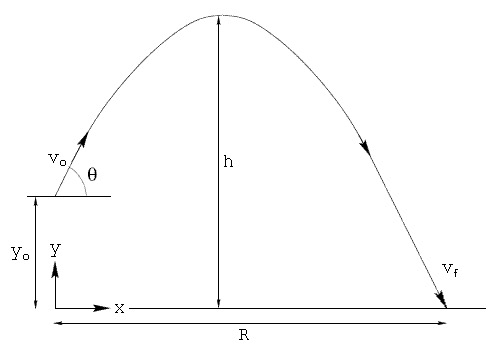
\includegraphics[width=0.45\linewidth]{pic/schieferwurf.png}
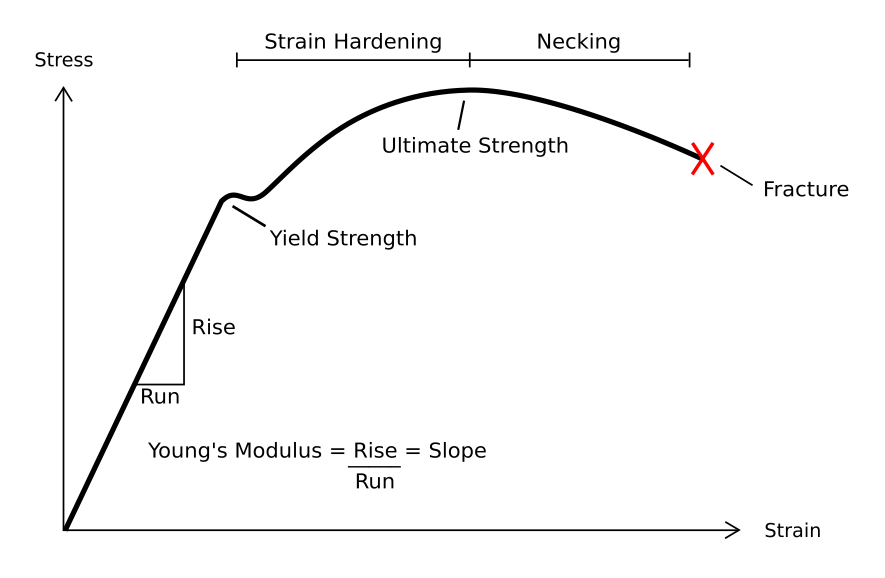
\includegraphics[width=0.5\linewidth]{pic/stressstrain.png}

\newpage
\subsection[Dynamik des Massenpunktes]{Dynamik des Massenpunktes\let\thefootnote\relax\footnote{$g$: Fallbeschleunigung $[\frac{m}{s^2}]$, $c_W$: Luftreibungskoeffizient, $D$: Direktionsmoment $[Nm]$, $q$: elektrische Ladung $[C]$, $E$: elektrisches Feld $[\frac{V}{m}]$, $B$: magnetische Flussdichte $[Am]$, $\varepsilon_0$: elektrische Feldkonstante $[\frac{As}{Vm}]$}}

\notes{Definition der Kraft: $\vec{F} = -\vec{\nabla}V = \d{\vec p}{t}$}

\concept{Kräfte}{
\f{Luftreibung}{F_R = \frac{1}{2} c_W A \rho v^2}\\

\f{Torsionsfederkraft}{F_D = -D \cdot \varphi}\\

\f{Lorentzkraft}{\vec{F} = q(\vec{E} + \vec{v} \times \vec{B})}\\

\f{Radialkraft}{F_R = -m \omega^2 r = -m \frac{v^2}{r}}\\

\f{Coulombkraft}{\vec{F}_{1,2} = \frac{q_1 \cdot q_2}{4 \pi \varepsilon_0 r_{12}^2} \cdot \frac{\vec{r_{12}}}{r_{12}}}\\

\fnote{Corioliskraft}{F_C = 2m(\vec{v} \times \vec{\omega})}{entsteht in sich drehendem Koordinatensystem}\\

\fnote{Stokesreibung}{\vec{F} = - \alpha \dot{\vec{r}}}{langsame sphärische Körper in Fluiden}\\

\fnote{Newtonreibung}{\vec{F} = -\beta v^2 \hat{\dot{r}}}{Platte, die über ein Fluid gezogen wird}\\

\f{Gleitreibung}{\vec{F} = -\mu F_{\perp} \hat{\dot{r}}}
}

\begin{center}
\begin{framed}
\noindent 1. Newton'sches Axiom: $\vec F = 0 \rightarrow \vec v = const.$\\
2. Newton'sches Axiom: $\vec{F} = m\vec{a} = \frac{d\vec{p}}{dt}$\\
3. Newton'sches Axiom: $\vec F_{A \rightarrow B} = - \vec F_{B \rightarrow A}$
\end{framed}
\end{center}

\concept{Kraft in rotierendem Koordinatensystem}{
$\vec{F}' = \vec{F} - m\dot{\vec{\omega}} \times \vec{r} - 2m\vec{\omega} \times \dot{\vec{\omega}}' - m\vec{\omega} \times (\vec{\omega} \times \vec{r})$
}

\conceptcon{Konservative Kräfte}{
$\vec{F}(\vec{r})$ ist konservativ, falls:}{
\begin{itemize}
\itemsep-0.5em
\item $\vec{F} = \vec{F}(r)$
\item $\vec\nabla \times \vec{F} = 0$
\item $\exists V(\vec{r}): \vec{F} = -\vec\nabla V$
\item Arbeit $-\int_C d\vec{r} \cdot \vec{F}$ wegunabhängig
\item $-\oint_C d\vec{r} \cdot \vec{F} = 0$
\end{itemize}
}




\subsection[Linearimpuls]{Linearimpuls\let\thefootnote\relax\footnote{$d$: Stoßparameter, $r$: Kugeldurchmesser, $I_{sp}$: spezifischer Impuls, $m_0$: Trockenmasse, $a$: durchschnittliche Halbachse, $\gamma$: Gravitationskonstante, $k$: Federkonstante $\units{N}{m}$, $D$: Federkonstante $[\frac{\text{N}}{\text{rad}}]$, $J_A$: Trägheitsmoment um andere Achse $[\text{kg} \text{m}^2]$}}


\concept{Linearimpuls}{
\f{für Massenpunkt}{\vec{p} = m \vec{v}}\\
\f{Vis-Viva-Gleichung}{v^2 = \gamma M (\frac{2}{r} - \frac{1}{a})}
}

\conceptcon{Elastischer Stoß}{Energie- und Impulserhaltungssatz gelten}{
\f{Geschwindigkeitsänderung}{\Delta v = 2 \frac{m_1 v_1 + m_2 v_2}{m_1 + m_2}}
\fnote{Stoßwinkel}{\sin(\alpha) = \big(\frac{d}{2r}\big)}{harte Kugeln}
}

\concept{Raketengleichung}{

\f{Ziolkowskigleichung}{\Delta v = I_{sp} g \cdot \ln \frac{m}{m_0}}

}


\subsection[Energie]{Energie\let\thefootnote\relax\footnote{}}

\concept{Arten von Energie}{
\f{Kinetische Energie}{E_{kin} = \frac{m}{2} v ^2}\\
\f{Höhenenergie}{E_{pot} = mgh}\\
\f{Spannenergie}{E_{spann} = \frac{1}{2}kx^2}
\f{Reibungswärme}{E_{R} = F_R s}\\
\f{Thermische Energie}{E_{therm} = \frac{f}{2} k_B T}\\
\f{Torsionsenergie}{E_{tors} = \frac{1}{2} D \varphi^2}\\
\f{Rotationsenergie}{E_{rot} = \frac{1}{2} J_A \omega^2}

}

\concept{Abgeleitete Größen}{

\f{Arbeit}{W = \vec{F} \cdot \vec{s} = -\int \vec{F} dx}\\
\f{Arbeitselement}{\delta W = -\vec{F} \cdot d\vec{r}}\\
\f{Gesamtenergie}{E = T + V}\\
\f{Leistung}{P = \d{W}{t} = \vec{F} \cdot \vec{v}}\\
}

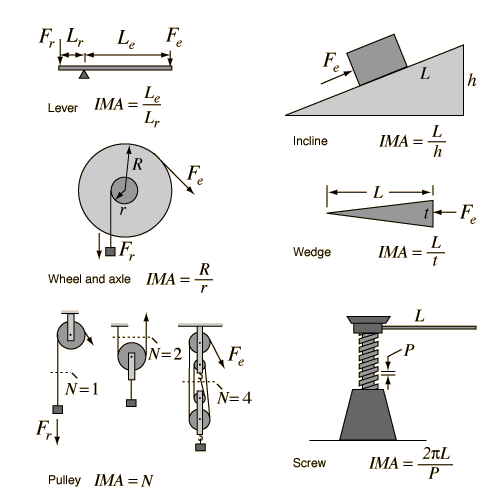
\includegraphics[width=0.5\linewidth]{pic/simplemach.png}
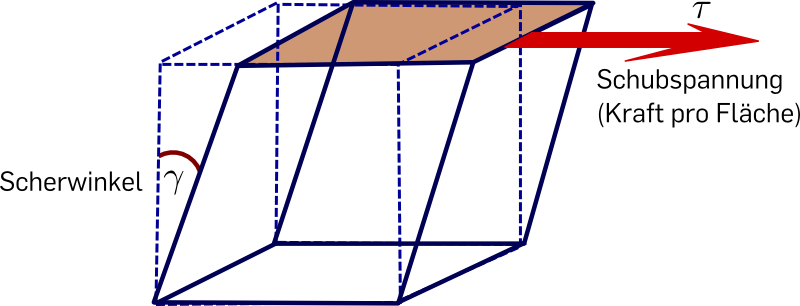
\includegraphics[width=0.5\linewidth]{pic/schubmodul.png}

\newpage
\subsection[Technische Mechanik]{Technische Mechanik\let\thefootnote\relax\footnote{$\delta$: Längenänderung [m], $A$: Angriffsfläche $[\text{m}^2]$, $\Delta_{max}$ maximale Deformation im Zentrum $[\text{m}]$, $\omega$: Kraft auf ganzen Balken $[\frac{\text{N}}{\text{m}}]$, $d_E$, $F_E$: Eingangsseite (effort), $d_R$, $F_R$: Ausgangsseite (reaction), pitch: Hubhöhe bei einer Umdrehung $[\text{m}]$, $U$: Umfang $[\text{m}]$, $N$: Anzahl Zähne, $t$: Drehmoment, $K$: Kompressionsmodul $[\frac{\text{N}}{\text{m}^2}]$, $G$: Schubmodul $[\frac{\text{N}}{\text{m}^2}]$, $\gamma$: Schubwinkel, $\nu$: Poissonzahl (Querkontraktionszahl)}}


\concept{Mechanische Größen}{

\f{Spannung}{\sigma = \frac{F}{A}}\\
\f{Verformung}{\epsilon = \frac{\delta}{l_0}}\\
\f{Young-Modulus}{E = \frac{\sigma}{\epsilon} = \frac{\sigma (F_2 - F_1) l_0}{(\delta_2 - \delta_1)A}}\\
\f{Deformation}{\delta = \frac{F l_0}{AE}}\\
\fnote{Biegung Balken}{\Delta_{max} = \frac{F l^3}{48 E}}{im Zentrum}\\
\fnote{Biegung Balken}{\Delta_{max} = \frac{5 \omega l^4}{384 E}}{gleichmäßig}
\f{Statik-Bedingung}{\sum_i \vec{F}_i = 0, \sum_i \vec{M}_i = 0}\\
\f{Kompressionsmodul}{K = -V \d{p}{V}}\\
\f{Kompressionsmodul}{K = \frac{E}{3(1-2 \nu)}}\\
\f{Kompressionskoeff.}{\kappa = \frac{1}{K}}\\
\f{Schubmodul}{G = \frac{E}{2(1+\nu)}}\\
\f{Schubspannung}{\tau = G \tan \gamma}\\
\f{Poissonzahl}{\nu = \frac{\Delta d /d}{\Delta l / l}}
}

\concept{Einfache Maschinen}{
\f{ideale Kraftersparnis}{IMA = \frac{d_E}{d_R}}\\
\f{wirkliche Kraftersparnis}{AMA = \frac{F_R}{F_E}}\\
\f{Flaschenzug}{IMA = \frac{\text{gezogene Länge}}{\text{bewegte Länge}}}\\
\f{Schiefe Ebene}{IMA = \frac{l}{h}}\\
\f{Keil}{IMA = \frac{l}{h}}\\
\f{Schraube}{IMA = \frac{U}{\text{pitch}}}\\
\f{Zahnradsystem}{GR_{tot} = (\frac{B}{A})(\frac{D}{C})}\\
\f{Übersetzungsverhältnis}{GR = \frac{N_{out}}{N_{in}} = \frac{d_{out}}{d_{in}} = \frac{\omega_{out}}{\omega_{in}} = \frac{t_{out}}{t_{in}}}\\
\f{Flaschenzugverhältnis}{FR = \frac{d_{out}}{d_{in}} = \frac{\omega_{in}}{\omega_{out}} = \frac{t_{out}}{t_{in}}}

}

\begin{center}
\begin{framed}
\centering Was man an Kraft spart, muss man an Weg zusetzen.
\end{framed}
\end{center}



\newpage
\subsection[Drehungen]{Drehungen\let\thefootnote\relax\footnote{$r$: Radius, $T$: Periodenlänge, $\omega$: Winkelgeschwindigkeit, $\alpha$: Winkelbeschleunigung, $J$: Trägheitsmoment um Achse oder Schwerpunkt}}


\concept{Kinematik}{

\f{Bogenlängenelement}{\Delta s = r \cdot \Delta \varphi}\\
\f{Winkelgrößen}{T = \frac{2 \pi}{\omega} = \frac{2 \pi r}{v} = \frac{1}{f}}\\
\f{Tangentialgeschwindigkeit}{\vec{v} = \vec{\omega} \times \vec{r}}\\
\f{Tangentialbeschleunigung}{\vec{\alpha_t} = \vec{\alpha} \times \vec{r}}\\
\f{Radialbeschleunigung}{\vec{\alpha_r} = \omega^2 \cdot \vec{r} = \frac{v^2}{r}}\\
}

\concept{Drehimpuls}{

\f{Gesamtdrehmoment}{J_S = \sum_i m_i r^2_i}\\
\f{Steiner'scher Satz}{J_A = J_S + m s^2}\\
\f{Massenschwerpunkt}{\vec{r}_M = \frac{\sum_i m_i \vec{r}_i}{\sum_i m_i}}\\
\f{Bewegungsgleichung}{\varphi(t) = \frac{1}{2} \alpha t^2 + \omega_0 t + \varphi_0}\\
\f{Drehmoment}{\vec{M} = \dot{\vec{L}} = \vec{r} \times \vec{F}}\\
\f{Drehmoment Betrag}{M = F \cdot r \cdot \sin(\varphi) = J_A \ddot{\varphi}}\\
\f{Drehimpuls}{\vec{L} = m \vec{r} \times \vec{v}}\\
}

\begin{center}
\begin{framed}
\begin{tabular}{ll}
Translation & Rotation\\
\midrule
$\vec{a} = \dot{\vec{v}} = \ddot{\vec{x}}$ & $\vec{\alpha} = \dot{\vec{\omega}} = \ddot{\vec{\varphi}}$\\
$W = -\int F_x dx$ & $W = -\int M_A d \varphi$ \\
$P = F_xv_x$ & $P = M_A \omega$ \\
$\vec{p} = m \cdot \vec{v}$ & $L_A = J_A \omega$ \\
\end{tabular}
\end{framed}
\end{center}

\begin{center}
\begin{framed}
\begin{tabular}{ll}
Trägheitsmoment & $J_S$\\
\midrule
Massepunkt & $mr^2$ \\
Vollzylinder & $\frac{1}{2}mr^2$ \\
Hohlkugel & $\frac{1}{2}m(r_2^2 - r_1^2)$ \\
Vollkugel & $\frac{2}{5}mr^2$ \\
Hohlkugel & $\frac{2}{3}mr^2$ \\
\makecell[l]{Stab um \\Schwerpunkt} & $\frac{1}{12}ml^2$ \\
Stab um Ende & $\frac{1}{3}ml^2$
\end{tabular}
\end{framed}
\end{center}


\subsection[Zentralkraftfeld]{Zentralkraftfeld\let\thefootnote\relax\footnote{$A$: überstrichene Fläche, $L$: Drehimpulsbetrag, $\dot \phi$: Winkelgeschwindigkeit, $a$: große Halbachse, $M$: Masse des größeren Körpers, $\gamma$: Gravitationskonstante, $R$: Radius Erde, $h$: Höhe des Orbits, $e$: Exzentrizität, $\Theta$: Streuwinkel, $\Omega$: Raumwinkel, $\sigma$: Wirkungsquerschnitt}}

\concept{Zentralpotential}{

\f{Rutherford'sche Streuformel}{\Theta = 2 \arcsin \frac{1}{\sqrt{1 + \frac{4 E^2 s ^2 }{\alpha ^2}}}}\\
\f{differentieller Wirkungsquerschnitt}{\d{\sigma}{\Omega} = \frac{\alpha ^2}{16E^2} \frac{1}{\sin^4 \frac{\Theta}{2}}}\\
\f{totaler Wirkungsquerschnitt}{\sigma_{tot} = 2\pi \frac{\alpha^2}{16E^2} \int_0^{\pi} \frac{\sin \Theta d\Theta}{\sin^4 \frac{\Theta}{2}}}
}

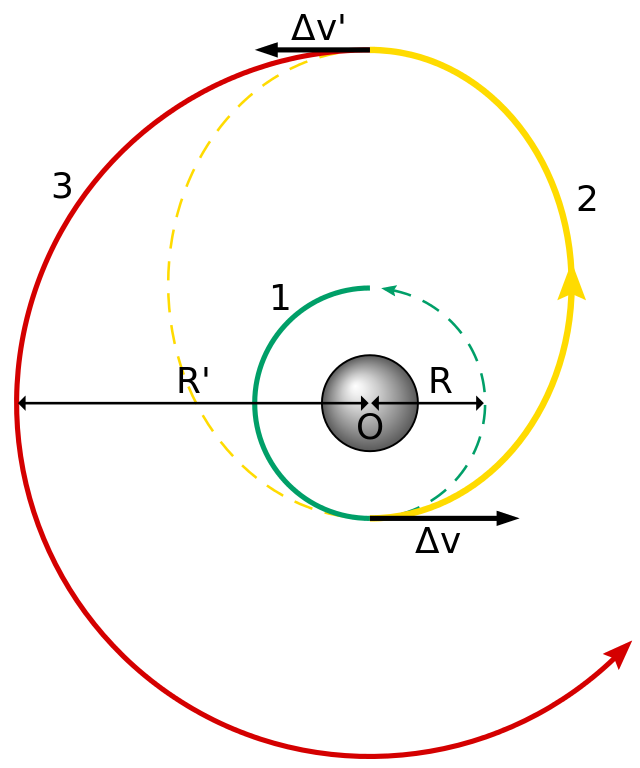
\includegraphics[width=0.45\linewidth]{pic/hohmann.png}
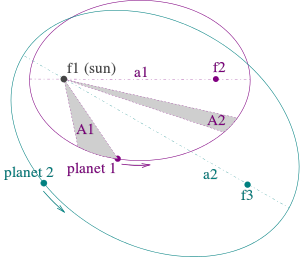
\includegraphics[width=0.45\linewidth]{pic/kepler.png}


\concept{Gravitation}{

\f{Zentralkraft}{\vec{F} = f(\vec{r}, \dot{\vec{r}}, t) \cdot \hat{r}}\\
\f{Flächenüberstreichung}{\Delta A = \frac{L}{2m} \Delta t}\\
\f{2. Keplersches Gesetz}{\d{A}{t} = \frac{1}{2} r^2 \dot{\phi} = \frac{L}{2m} = const.}\\
\f{3. Kepler'sches Gesetz}{\frac{T^2}{a^3} = \frac{4 \pi^2}{\gamma M} = const.}\\
\f{Gravitationspotential}{V = - \frac{\gamma M m}{r}}\\
\f{Gravitationskraft}{\vec{F}_{G12} = - \gamma \frac{m_1 \cdot m_2}{r_{12}^2} \cdot \frac{\vec{r_{12}}}{r_{12}}}\\
\f{Gesamtenergie}{E = \frac{1}{2}mv^2 - \gamma \frac{m \cdot m_0}{r} = const.}\\
\f{1. kosmische Geschwindigkeit}{v_1 = \sqrt{\frac{2 \gamma M}{R}}}\\
\f{2. kosmische Geschwindigkeit}{v_2 = \sqrt{\frac{\gamma M}{R}}}\\
\f{Umlaufzeit}{T_S(h) = 2 \pi \sqrt{\frac{R}{g}(1+\frac{h}{R})^3}}\\
\f{Bahngeschwindigkeit}{v(h) = \sqrt{gR \Big(\frac{1}{1+\frac{h}{R}}\Big)}}\\
\f{Ellipse}{e^2 = a^2-b^2}\\
\f{numerische Exzentrität}{\varepsilon = \frac{e}{a}}\\

}


\subsection[Mehrteilchensysteme]{Mehrteilchensysteme\let\thefootnote\relax\footnote{$\mu$: reduzierte Masse}}


\concept{Mehrteilchensysteme}{

\f{Bewegungsgleichung}{m_i \ddot{\vec{r}}_i = \vec{F}_i^{(ex)} + \sum_j \vec{F}_{ij}}\\
\f{reduzierte Masse}{\mu = \frac{m_1 m_2}{m_1 + m_2}}\\
\f{Schwerpunktssatz}{M \ddot{\vec{R}} = \vec{F}^{(ex)}}\\
\f{Schwerpunkt}{\vec{R} = \frac{m_1 \vec{r}_1 + m_2 \vec{r}_2}{m_1 + m_2}}\\
\f{Impulssatz}{\dot{\vec{p}} = \vec{F}^{ex}}\\
\f{Drehmoment}{\dot{\vec{L}} = \sum_i \vec{r}_i \times \vec{F}_i^{ex}}\\
\f{kinetische Energie}{T = \sum_i \frac{1}{2} m_i \dot{\vec{r}}_i \cdot \dot{\vec{r}}_i}\\
\f{konservative Kräfte}{\d{T}{t} = - \d{V}{t}}\\
\f{Schwerpunktsbewegung}{\vec{R}(t) - \frac{\vec{p}}{M}t = \vec{R}(0) = const.}\\
\f{Virialsatz}{2 \langle T \rangle = \langle \sum_i \vec{r}_i \cdot \nabla_i V \rangle}\\
\f{Gesamtenergie}{\frac{M}{2} \dot{\vec{r}}_0^2 + \frac{1}{2} \sum_i m_i (\vec{\omega} \times \vec{r}_i)^2}\\
\f{Drehimpuls}{\vec{L} = \overleftrightarrow{J}\vec{\omega}}\\
\f{Rotationsenergie}{T_R = \frac{1}{2} \vec{\omega} \cdot \vec{L}}\\
\f{Trägheitstensor}{J_{lm} = \int d^3 r \rho(\vec{r}) (\delta_{lm} \vec{r}^2 - x_l x_m)}\\
\f{Drehmoment}{\vec{M} = \overleftrightarrow{J} \dot{\vec{\omega}} + \vec{\omega} \times \overleftrightarrow{J} \vec{\omega}}\\
\f{Präzession}{\omega_P = \frac{m g r}{J \omega}}

}

\begin{center}
\begin{framed}
Jede 3D-Transformation mit Fixpunkt kann als Rotation um eine Achse beschrieben werden. (Jeder Rotationsmatrix mit Fixpunkt hat Eigenwerte $\pm 1$.)\\
\textsc{Euler'scher Satz}
\end{framed}
\end{center}

\subsection[Relativitätstheorie]{Relativitätstheorie\let\thefootnote\relax\footnote{$\gamma$: Lorentzfaktor}}

\begin{framed}
\centering
$\gamma = \dfrac{1}{\sqrt{1 - \beta^2}} > 1$ und $\beta = \frac{v}{c} <1$
\end{framed}

\begin{center}
\begin{framed}
\begin{tabular}{ll}
Galileo-Trafo & $\vec{r} = \vec{V}t + \vec{r}'$, $t = t'$\\
Zeitabl. Galileo-Trafo & $\d{}{t} = \Big(\d{}{t}\Big)' + \vec{\omega} \times$\\
Addition von Geschw. & $v_{tot} = \frac{v_1 + v_2}{1 + \frac{v_1 v_2}{c^2}} < c$\\
\end{tabular}
\end{framed}
\end{center}

\begin{center}
\begin{framed}
\begin{tabular}{ll}
$x\prime=\gamma(x - v_xt)$ & $x=\gamma(x\prime+v_xt)$ \\
$y\prime=y$ & $y=y\prime$\\
$t\prime=\gamma(t-v_x \frac{x}{c^2})$ & $t=\gamma(t\prime+v_x \frac{x\prime}{c^2})$\\
\end{tabular}
\end{framed}
\end{center}

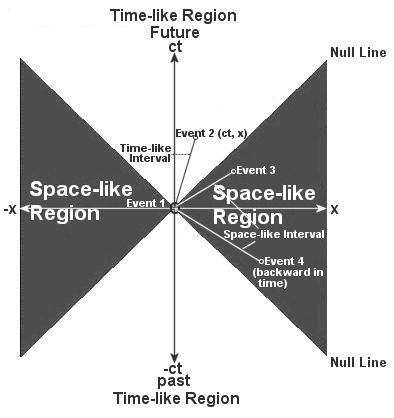
\includegraphics[width=0.45\linewidth]{pic/minkowski.jpg}

\concept{Grundlagen}{

\f{metrischer Tensor}{\begin{aligned} a^{\mu} &= g^{\mu \nu} a_{\nu}\\ a_{\mu} &= g_{\mu \nu} a^{\mu}\end{aligned}}\\
\f{allg. Lorentztrafo}{\underline{x}_{\mu} = L_{\mu}^{\,\ \nu} x_{\nu} \text{ und } \underline{x}^{\mu} = L^{\mu}_{\,\ \nu} x^{\nu}}\\
\f{kontravariant}{(a^0, a^1, a^2, a^3) = (a^0, \vec{a})}\\
\f{kovariant}{(a_0, a_1, a_2, a_3) = (a^0, -\vec{a})}\\
\f{Skalarprodukt}{a_{\mu} b^{\mu} = a^{\mu}b_{\mu} = a^0b^0 - \vec{a} \cdot \vec{b}}\\
\f{Betragsquadrat}{a_{\mu} a^{\mu} = (a^0)^2 - \vec{a} \cdot \vec{a}}\\
\f{Vierervektorquadrat}{s^2 = c^2 t^2 - \vec{r}^2}\\
\f{zeitartig}{\Delta s^2 > 0}\\
\f{lichtartig}{\Delta s^2 = 0}\\
\f{raumartig}{\Delta s^2 < 0}\\
\f{Vierergeschwindigkeit}{u^0 = \gamma c$ und $\vec{u} = \gamma \vec{v}}\\
\f{Geschwindigkeitsquadrat}{u_{\mu} u^{\mu} = c^2}\\
\f{Viererbeschleunigung}{a_{\mu} a^{\mu} = -\gamma^4 \Big[\gamma^2 \Big( \frac{\vec{v}}{c} \cdot \vec{a} \Big)^2 + \vec{a}^2 \Big]}

}

\begin{center}
\begin{framed}
$g^{\mu \nu} =
\Bigg(\begin{smallmatrix}
1 & 0 & 0 & 0\\
0 & -1 & 0 & 0\\
0 & 0 & -1 & 0\\
0 & 0 & 0 & -1
\end{smallmatrix}\Bigg)$
und $L^{\mu}_{\,\ \nu} = \Bigg(\begin{smallmatrix}
\gamma & -\beta \gamma & 0 & 0\\
-\beta \gamma & \gamma & 0 & 0\\
0 & 0 & 1 & 0\\
0 & 0 & 0 & 1
\end{smallmatrix}\Bigg)$
\end{framed}
\end{center}

\concept{Energie}{

\f{Gesamtenergie}{E^2 = m_0^2 c^4 + c^2p^2}\\
\f{relativistische Energie}{E = \gamma m_0 c^2}\\
\f{relativistischer Impuls}{p = \gamma m_0 v}\\
\f{Zeitdilatation}{\Delta t = \gamma \Delta \tau}\\
\f{Lorentzkontraktion}{l = \frac{l_0}{\gamma}}\\
\f{Newton}{m \d{u^{\mu}}{\tau} = ma^{\mu} = K^{\mu}}\\
\f{Kraft}{\vec{K} = \gamma \vec{F}$, $K^0 = \gamma \frac{\vec{F} \cdot \vec{v}}{c}}\\
\f{Lagrange}{\d{}{\tau} \pd{\mathscr{L}}{u^{\mu}} - \pd{\mathscr{L}}{x^{\mu}} = 0}
}

\concept{Felder}{

\f{Divergenz}{\pd{x^{\mu}}{x^{\mu}} = 4}\\
\f{Nabla}{\begin{aligned} &(\partial_0, \partial_1, \partial_2, \partial_3) = \Big(\frac{1}{c} \pd{}{t}, \vec{\nabla}\Big)\\
&(\partial^0, \partial^1, \partial^2, \partial^3) = \Big(\frac{1}{c} \pd{}{t}, -\vec{\nabla}\Big)\end{aligned}}\\
\f{em. Feld}{\mathscr{L} = \frac{m}{2} v^2 + \frac{q}{c} \vec{v} \cdot \vec{A} - q \phi}\\
\f{Vektorpotential}{(A_0, A_1, A_2, A_3) = (\phi, - \vec{A})}\\
\f{Invarianten}{E^2 + H^2, \vec E \cdot \vec H}\\
\f{Dopplereffekt}{\omega' = \omega_s (1-\beta)\gamma}

}

\begin{center}
\begin{framed}

$E_y = \gamma (E_y' + \beta H_z')$, $H_y = \gamma (H_y' - \beta E_z')$\\
$E_z = \gamma (E_z' - \beta H_y')$, $H_z = \gamma (H_z' + \beta E_y')$\\
$\varphi = \gamma(\varphi' + \beta A_x')$, $A_x' = \gamma(A_x - \frac{\beta}{c} \varphi)$

\end{framed}
\end{center}

\subsection[Fluide]{Fluide\let\thefootnote\relax\footnote{$A$: Querschnittsfläche Rohr, $I$: Volumenstrom, $g$: Fallbeschleunigung, $\eta$: dynamische Viskosität $[\text{Pa}~\text{s}]$, $\sigma$: Oberflächenspannung $[\frac{\text{N}}{\text{m}}]$, $h$: Steighöhe, $\varphi$: Winkel Oberfläche mit Gefäßwand}}


\concept{Fluide}{

\f{Druck}{p = \frac{F}{A}}\\
\f{Dichte}{\rho = \frac{m}{V}}\\
\f{Bernoulli-Gesetz}{\overbrace{p_0}^\textrm{stat.} + \overbrace{\frac{1}{2}\rho v^2}^\textrm{dynam.} + \overbrace{\rho g y}^\textrm{pot.} = const.}\\
\f{Kontinuitätsgleichung}{A_1 v_1 = A_2 v_2 = I = \frac{dV}{dt}}\\
\f{Archimedisches Prinzip}{F_A = m_F g = \rho_F V_K g}\\
\f{Volumenstrom Rohr}{\dot{V} = \frac{\pi r^4 \Delta p}{8 \eta l}}\\
\f{Reibung Rohrströmung}{F_R = 8\pi\eta l \bar{v}}\\
\f{laminarer Strömungswiderstand}{F_R = 6 \pi \eta r v}\\
\f{Höhenformel}{p(z) = p_0 \cdot e^{-\frac{\rho_0 g z}{p_0}}}\\
\f{Dichtebestimmung}{\rho_K = \rho_{F} \cdot \frac{|\vec{F_{G,L}}|}{|\vec{F_{G,L}}|-|\vec{F_{G,F}}|}}\\
\f{Oberflächenspannung}{\sigma = \frac{dW}{dA} = \frac{F}{2l}}\\
\f{Kapillareffekt}{h = \frac{2 \sigma \cos(\varphi)}{\rho r g}}

}


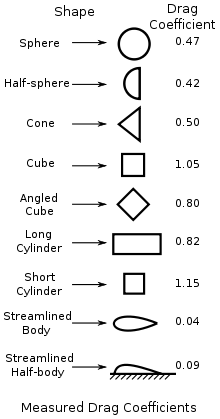
\includegraphics[width=0.45\linewidth, angle=90]{pic/luftcw.png}


\subsection[Schwingungen und Wellen]{Schwingungen und Wellen\let\thefootnote\relax\footnote{$\gamma$: Dämpfungsterm, $K$: Kompressionsmodul, $\rho$: Dichte, $P_S$: Schallleistung, $v$: Geschwindigkeit des Körpers, $c_s$: Schallgeschwindigkeit, $Ma$: Mach-Zahl, $b$: Reibungskoeffizient}}

\begin{framed}
$$\ddot{x} + \underbrace{2 \gamma \dot{x}}_\text{Dämpfung} + \omega_0^2 x = \underbrace{\omega_0^2 x_0 \sin(\omega_A t)}_\text{Anregung}$$
\end{framed}

\concept{Schwingung}{

\f{harmonische Schwingung}{x(t) = x_m \cos(\omega t + \alpha)}\\
\f{Frequenz}{\omega = \sqrt{\omega_0^2 - \gamma^2}}\\
\f{Schwebung}{\Delta \omega = \omega_1 - \omega_2}\\
\f{Potentialnäherung}{V(x) \cong V(x_0) + \frac{1}{2} \kappa (x-x_0)^2}
}

\begin{center}
\begin{framed}
$$k = \frac{2 \pi}{\lambda}$$
$$c =  \frac{\omega}{k} = \lambda f = \frac{\lambda}{T}$$
\end{framed}
\end{center}

\concept{Wellen}{

\f{1D-Welle}{y(x,t) = y_m \sin(kx - \omega t)}\\
\f{Gütefaktor}{Q = \frac{\omega_0}{\Delta \omega}}\\
\f{Gesamtenergie}{E_{ges} = \frac{k}{2}A^2}\\
\f{abklingende Energie}{E = E_0 e^{-\frac{t}{\tau}}}\\
\f{Transmissionskoeffizient}{T = \frac{2v_2}{v_2 + v_1}}\\
\f{Reflexionskoeffizient}{R = \frac{v_2 - v_1}{v_2 + v_1}}\\
\f{Absorptionskoeffizient}{A = 1 - R - T}\\
\f{mittlere Leistung}{P_{gem} = \frac{1}{2}\mu v \omega^2 y_m^2}\\
\f{Schallgeschwindigkeit}{v = \sqrt{\frac{K}{\rho}}}\\
\f{Schallintensität}{I = \frac{1}{2} \rho v \omega^2 s_m^2$, $I = \frac{P_S}{4 \pi r^2}}\\
\fnote{stehende Wellen}{f = \frac{v}{\lambda} = \frac{nv}{2l}}{feste Enden}
\fnote{stehende Wellen}{f = \frac{v}{\lambda} = \frac{nv}{4l}}{loses Ende}\\
\f{Mach'scher Kegel (halb)}{\sin(\alpha) = \frac{c_S}{v} = \frac{1}{Ma}}\\
\f{Reibung}{F_R = -b \dot{z}$, $\gamma = \frac{b}{2m}}

}


\subsection[Lagrange]{Lagrange\let\thefootnote\relax\footnote{$N$: Teilchenzahl, $p$: Zwangsbedingungen, $S$: Wirkung}}

\concept{Lagrange}{

\f{skleronom (rheonom)}{\pd{f}{t} = (\neq) 0}\\
\f{holonom}{\d{}{t} \pd{T}{\dot{q}_j} - \pd{T}{q_j} = Q_j}
\f{Freiheitsgrade}{S = 3N - p}\\
\f{Bewegungsgleichung}{m_i \ddot{\vec{r}}_i = \vec{Z}_i + \vec{K}_i}\\
\f{virtuelle Verrückung}{\delta \vec{r}_i(t) = \vec{r}'_i(t) - \vec{r}_i(t)}\\
\f{d'Alembert}{\sum_i (\vec{K}_i - \dot{\vec{p}}_i) \cdot \delta \vec{r}_i = 0}\\
\f{generalisierte Kräfte}{Q_j = \sum_{i = 1}^N \vec{K}_i \cdot \pd{\vec{r}_i}{q_j}}\\
\f{d'Alembert (generalisiert)}{\sum_{i = 1}^S \Big\{ \d{}{t} \pd{T}{\dot{q}_j} - \pd{T}{q_j} - Q_j \Big\} \delta q_j = 0}\\
\f{Gleichgewicht}{\sum_i Q_i \delta q_i = 0}\\
\f{Lagrange-Gleichung 2. Art}{\d{}{t} \pd{\mathscr{L}}{\dot{q}_j} - \pd{\mathscr{L}}{q_j} = 0}\\
\f{Lagrange em. Feld}{\mathscr{L} = \frac{1}{2}m \dot{\vec{r}}^2 - q (\phi + \dot{\vec{r}} \cdot \vec{A})}\\
\f{Euler'sche Gleichung}{\pd{f}{y} - \d{}{x}\pd{f}{y'} = 0}\\
\f{konjugierter Impuls}{p_j = \pd{\mathscr{L}}{\dot{q}_j}}\\
\f{zyklische Koordinaten}{\pd{\mathscr{L}}{q_j} = 0}\\
\f{Hamilton-Funktion}{H = \sum_j p_j \dot{q}_j - \mathscr{L}}\\
\f{Totale Zeitableitung Hamiltonian}{\d{H}{t} = 0 = \pd{H}{t}}\\
\f{Rayleigh'sche Dissipationsfunktion}{P = \sum_{i=1}^N \int_0^{v_i} dv'_i R_i(v'_i)}
\\
\f{Reibungskräfte}{Q_j^{(R)} = -\pd{P}{\dot{q}_j}}\\
\f{Lagrange-Gleichung 1. Art}{\d{}{t} \pd{\mathscr{L}}{\dot{q}_j} - \pd{\mathscr{L}}{q_j} = \sum_{\nu = 1}{k} \lambda_{\nu} a_{\nu j}}
}

\begin{framed}
\begin{center}
\textbf{\textsc{Noether}-Theorem}: Zu jeder kontinuierlichen Symmetrie eines physikalischen Systems gehört eine Erhaltungsgröße.\\
\begin{tabular}{ll}
Zeit homogen & $H = const.$,\\
Raum homogen & $\vec{p} = const.$,\\
Raum isotrop & $\vec{L} = const.$
\end{tabular}
\end{center}
\end{framed}

\begin{framed}
\noindent
$$\mathbf{\delta \mathcal{S} =} \delta \int_{t_1}^{t_2} dt \mathscr{L}\mathbf{= 0}$$
\begin{center}\textsc{Weltformel}\end{center}
\end{framed}

\newpage
\subsection[Hamilton]{Hamilton\let\thefootnote\relax\footnote{}}

\begin{framed}
\begin{tabular}{ll}
Poissonkl. mit H & $\d{f}{t} = \{f, H\} + \pd{f}{t}$\\
Beliebige Poissonkl. & $\{f, g\}_{\vec{q}, \vec{p}} = \sum_{j=1}^S \Big( \pd{f}{q_j} \pd{g}{p_j} - \pd{f}{p_j} \pd{f}{q_j}\Big)$\\
$f$ Erhaltungsgröße & $\{f, H\} = 0$\\
$f$, $g$ erhalten & $\{f, g\}$ auch.\\
\end{tabular}
\end{framed}

\begin{center}
\begin{framed}
\begin{itemize}
\itemsep-0.5em
\item $\{f,g\}_{\vec{q}, \vec{p}} = \{f,g\}_{\vec{Q}, \vec{P}}$
\item $\{f, f\} = 0$
\item $\{f,g\} = -\{g, f\}$
\item $\{f+g, h\} = \{f,h\} + \{g, h\}$
\item $\{fg, h\} = f\{g,h\} + \{f,h\}g$
\item $\{\{f,g\}h\} + \{\{g,h\}, f\} + \{\{h,f\}, g\} = 0$
\end{itemize}
\end{framed}
\end{center}

\begin{center}
\begin{framed}
\begin{tabular}{l|l|l}
$F_1(\vec{q}, \vec{Q}, t)$ & $p_j = \pd{F_1}{q_j}$ & $P_j = - \pd{F_1}{Q_j}$\\
$F_2(\vec{q}, \vec{P}, t)$ & $p_j = -\pd{F_2}{q_j}$ & $Q_j = \pd{F_2}{P_j}$\\
$F_3(\vec{p}, \vec{Q}, t)$ & $q_j = -\pd{F_3}{p_j}$ & $P_j = - \pd{F_3}{Q_j}$\\
$F_4(\vec{p}, \vec{P}, t)$ & $q_j = -\pd{F_4}{p_j}$ & $Q_j = \pd{F_4}{P_j}$\\
\end{tabular}
\end{framed}
\end{center}

\begin{center}
\begin{framed}

$\begin{aligned}
\{q_i, q_j\} &= 0 \quad\\
\{p_i, p_j\} &= 0\\
\{q_i, p_j\} &= \delta_{ij}
\end{aligned}$\\
fundamentale Poissonklammern

\end{framed}
\end{center}

\begin{center}
\begin{framed}
\noindent\begin{tabular}{ll}
Legendre 1 & $g(u) = f(x) -ux = f(x) - x \d{f}{x}$\\
Legendre 2 & $g(x,v) = f(x,y) - vy = f(x,y) - y (\pd{f}{y})_x$\\
Legendre H & $H = p\dot{q} - L = p \dot{q}^\star-\mathscr{L}^\star$\\
Liouville'scher Satz & $\d{\rho}{t} = 0$\\
\end{tabular}
\end{framed}
\end{center}

\newpage
\section{Statistik}

\begin{framed}
$$n! \sim \sqrt{2\pi n} \big(\frac{n}{e}\big)^n$$
$$\ln(n!) = n \ln(n) - n$$
\centering\textsc{Stirling-Formel}
\end{framed}


\subsection[Wahrscheinlichkeitsverteilungen]{Wahrscheinlichkeitsverteilungen\let\thefootnote\relax\footnote{}}

\concept{Binomialverteilung}{

\f{Wahrscheinlichkeit für Ereignis i}{p_i = \lim_{N \rightarrow \infty} \frac{N_i}{N}}\\
\f{Realitätsbedingung}{\sum_i p_i = 1}\\
\f{Addition von Wahrscheinlichkeiten}{P(i \lor j) = P_{i+j} = P_i + P_j}\\
\f{Multiplikation von Wahrscheinlichkeiten}{P(i \land j) = P_{ij} = P_i \cdot P_j}\\
\f{charakteristische Funktion}{\varphi (k) = \int \exp(ikx) w(x) dx}\\
\f{r-tes Moment aus charakt. Funktion}{\bar{x^r} = (-i)^r \frac{\text{d}^r}{\text{d}k^r} \varphi(k)|_{k=0}}\\
\f{Binomialkoeffizienten}{{N \choose n} = \frac{N!}{(N-n)! n!}}\\
\f{Gesetz der großen Zahlen}{\frac{\Delta A}{\bar A} \longrightarrow 0}
}

\begin{center}
\begin{framed}
\noindent\begin{tabular}{lll}
 & diskrete Verteilung & kontinuierliche Verteilung\\
\midrule
Norm $1$ & $\sum_i p_i$ & $\int w(x) dx$\\
Mittelwert $\bar x$ & $\langle x \rangle = \sum_i x_i p_i$ & $\int x w(x) dx$\\
r-tes Moment $\bar {x^r}$ & $\sum_i x_i^r p_i \neq {\bar x}^r$ & $\int x^r w(x) dx$\\
Varianz $(\Delta x)^2$ & $\bar{x^2} - \bar{x}^2$ & $\int x^2 w(x) dx - (\int x w(x) dx)^2$
\end{tabular}
\end{framed}
\end{center}

\begin{center}
\begin{framed}
\noindent\begin{tabular}{llll}
 & Binomalverteilung & Normalverteilung & Poissonverteilung\\
\midrule
Verteilung $P(n)$ & ${N \choose n} p^n q^{N-n}$ & $ \frac{1}{\sqrt{2\pi}\sigma} \exp{-\frac{(n-\bar{n})^2}{2\sigma^2}}$ & $\frac{\lambda^n}{n!} e^{-\lambda}$\\
Mittelwert $\bar{n}$ & $pN$ & $pN$ & $pN$\\
Varianz $(\Delta n)^2$ & $pqN$ & $pqN$ & $pN$\\
Gültigkeit & exakt & \makecell[l]{$\bar n = Np \gg 1$ \\ $N - \bar n = Nq \gg 1$} & $p \ll  \text{ und } n \ll N$\\
\end{tabular}
\end{framed}
\end{center}

\subsection[Grundlagen]{Grundlagen\let\thefootnote\relax\footnote{}}

\noindent Ein \textbf{Mikrozustand} oder ein reiner Zustand $r$ beschreibt ein System vollständig, ohne jeglichen Informationsverlust.\\

\noindent Ein \textbf{Makrozustand} oder gemischter Zustand $\{P_r\}$ beschreibt ein System unvollständig und ist durch die Angabe der Wahrscheinlichkeiten $P_r$, mit denen bestimmte Mikrozustände $r$ eines Systems vorkommen können, festgelegt.\\

\noindent \textbf{Erreichbare} Mikrozustände sind alle die Zustände, die in einem gegebenen Makrozustand vorkommen können bzw. mit diesem verträglich sind. Sie müssen grundsätzlich abzählbar sein.\\

\begin{center}
\begin{framed}
\noindent In einem abgeschlossenen System ($E, V, N = $ const., d.h. mikrokanonisches Ensemble) im Gleichgewicht sind alle $\Omega$ erreichbaren Zustände $r$ gleichwahrscheinlich, d.h. es gilt $P_r = \frac{1}{\Omega}$
\end{framed}
\end{center}

\concept{Statistische Thermodynamik}{
\f{Planck-Zelle}{\tau = (2\pi \hbar)^f = h^f}\\
\f{Gibbs-Faktor}{\frac{1}{N!}}\\
\f{Ergodenhypothese}{\bar A^T = \bar A}\\
\f{statistische Entropie}{S = k \ln \Omega}\\
\f{Volumen einer N-dimensionale Kugel}{V_N(R) = \frac{\pi^{N/2}}{(\frac{N}{2})!}R^N}\\
\f{thermische Wellenlänge}{\lambda = \frac{h}{\sqrt{2\pi m k T}}}
}

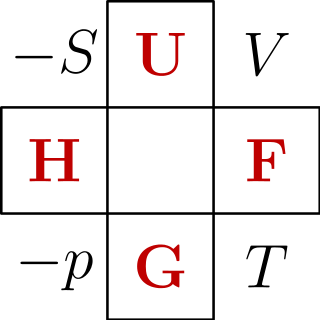
\includegraphics[width=0.5\linewidth]{pic/suv.png}
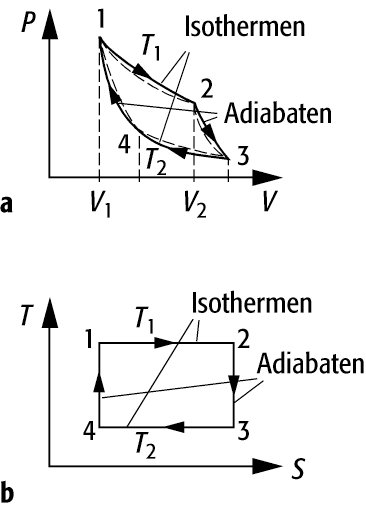
\includegraphics[width=0.4\linewidth]{pic/kreisprozess.jpg}

\subsection{Dichteoperator}

\concept{Dichteoperator}{
\f{Dichteoperator}{\hat \rho = \sum_r P_r \ket{\psi_r}\bra{\psi_r}}
}

\subsection{Entropie}

\textbf{Fundamentalpostulat}: Im Gleichgewicht eines abgeschlossenen Systems ist die Entropie maximal.\\
\textbf{Extremalprinzip}: Im Gleichgewicht ist für alle Systeme die Entropie maximal: $\dbar S = 0$

\begin{center}
\begin{framed}
	\begin{tabular}{ll}
	Entropie & \\
	\midrule
	Thermodynamisch & $\dbar Q = T dS$\\
	Statistisch & $S = k \ln \Omega(E, X)$\\
	Informationstheoretisch & $S = - k \sum_i w_i \ln w_i$\\
	\midrule
	im Quantensystem & $S = -k \tr(\hat \rho \ln \hat \rho) = -k \langle \ln \hat \rho \rangle$\\
	im klassischen System & $S = -k \int dq dp \rho(q, p) \ln [\tau \rho(q, p)]$\\
	\bottomrule
	\end{tabular}
\end{framed}
\end{center}

\subsection[Ensembles]{Ensembles\let\thefootnote\relax\footnote{}}

Ein \textbf{Ensemble} ist ein gedachtes Kollektiv vieler gleichartiger Systeme, in dem die zugänglichen Mikrozustände mit geforderten Nebenbedingung verträglich sind, mit bestimmten Wahrscheinlichkeiten vorkommen und den Makrozustand beschreiben. Im thermodynamischen Limit ($N \longrightarrow \infty$, $V \longrightarrow \infty$, $\frac{N}{V} = $ const.) sind alle Ensembles identisch und liefern die gleichen thermodynamischen Beziehungen.\\

\begin{center}
\begin{framed}
	\noindent \begin{tabular}{lllll}
	Ensemble & Konstanten & Variablen & Zustandssumme & Dichteoperator $\hat \rho$\\
	\midrule
	Mikrokan. E. & E, N, V & E, N, V & $\sum_{r: E-\Delta E \leq E_r \leq E} 1$ & $\frac{1}{\Omega} \sum_r \ket{\Phi_r}\bra{\Phi_r}$\\
	Kan. E. & $\langle E \rangle$, N, V & T, N, V & $\sum_r e^{-\beta E_r} = \tr e^{-\beta \hat H}$ & $\frac{e^{-\beta \hat H}}{Z}$\\
	Großkan. E. & $\erw{E}, \erw{N}, V$ &  T, $\mu$, V & $\sum_r e^{-\beta(E_r \mu N_r)}$ & $\frac{e^{-\beta(\hat H - \mu \hat N)}}{Y}$\\
	\end{tabular}
\end{framed}
\end{center}

\newpage
\section{Thermodynamik}
\subsection[Grundbegriffe]{Grundbegriffe\let\thefootnote\relax\footnote{$R$: Gaskonstante $= 8.314 \frac{\text{J}}{\text{K}\text{mol}}$, $k_B$: Boltzmannkonstante, $N_A$: Avogadrozahl, $C_p, C_V$: Wärmekapazität bei konstantem Druck/Volumen}}

%
% \begin{framed}
% 	\begin{tabular}{|c|c|c|c|}
% 	\midrule
% 	 & $^{\circ}C$ & $^{\circ}K$ & $^{\circ}F$\\
% 	\midrule
% 	$^{\circ}C$ & C & $C + 273,15$ & $\frac{9}{5}C + 32$\\
% 	$^{\circ}K$ & $K - 273,15$ & K & $\frac{9}{5}(K - 273.15) + 32$\\
% 	$^{\circ}F$ & $\frac{5}{9}(F - 32)$ & $\frac{5}{9}(F - 32) + 273,15$ & F\\
% 	\midrule
% 	\end{tabular}
% \end{framed}

\concept{Grundgrößen}{
\f{ideales Gas}{\boxed{pV = nRT} = k_B N T = N_A n k_B T}\\
\f{reales Gas}{(p+\frac{an^2}{V^2} (V - bn) = nRT}\\
\f{Poisson-Konstante}{\gamma = C_p / C_V}\\
\f{Gaskonstante}{R = C_p - C_V}\\
\f{adiabatische Zustandsgl.}{TV^{\gamma-1} = const.}\\
\f{}{PV^{\gamma} = const.}\\
\f{Wirkungsgrad}{\eta = \frac{\Delta W}{Q}}\\
\f{Druck}{p = \frac{F_{\perp}}{A}}\\
\f{Wärmestrom}{I = \frac{dQ}{dt} = \lambda A \frac{dT}{dx}}\\
\f{Wärmedichte}{j = \frac{\dot{Q}}{A} = \lambda \frac{\Delta T}{l}}\\
\f{thermische Energie}{E_{kin} = \frac{1}{2} m \bar{v}^2  = \frac{1}{2} R T \text{ (pro Mol)} = \frac{3}{2} k_B T \text{ (pro Teilchen) }}\\
\f{Wärmekapazität}{\text{d}Q = C dT}\\
\f{Wärmemenge}{Q = C \cdot \Delta T}\\
\f{innere Energie}{\Delta U = Q + W}}

\concept{Entropie}{
\f{Entropieänderung}{\oint dS = 0}\\
\f{reversibler Prozess}{dS_{rev} = \frac{dQ_{rev}}{T}}\\
\f{Entropie}{\Delta S = C_V \cdot \ln \frac{T_2}{T_1} + nR \cdot \ln \frac{V_2}{V_1}}\\
\f{Entropie}{S = k_B \cdot \ln P^{-1} = k_B \cdot \ln \Omega(M)}
}

\concept{Wärmekraftmaschinen}{
\f{Längenausdehnung}{dl = \alpha l dT}\\
\f{Volumenausdehnung}{dV = \gamma V dT}\\
\f{Kompressionsarbeit}{W = -\int_{V_1}^{V_2} p dV}\\
\f{Wirkungsgrad}{\eta_C = \frac{|W|}{Q_w} = \frac{Q_w + Q_k}{Q_w} = \frac{T_w - T_k}{T_w}}\\
\f{Kältemaschine}{C_L = \frac{Q_k}{W} = \frac{Q_k}{|Q_w| - Q_k} = \frac{T_k}{T_w - T_k}}\\
\f{Wärmepumpe}{C_L = \frac{|Q_w|}{W} = \frac{|Q_w|}{|Q_w| - Q_k} = \frac{T_w}{T_w - T_k}}
}

\subsection[Hauptsätze]{Hauptsätze\let\thefootnote\relax\footnote{}}

\begin{center}
\begin{framed} \noindent Für jedes thermodynamische System existiert eine intensive Zustandsgröße, die Temperatur $T$. Ihre Gleichheit ist notwendige Voraussetzung für das thermische Gleichgewicht zweier Systeme.
\begin{center} 0. Hauptsatz\end{center}\end{framed}
\end{center}

\begin{center}
\begin{framed}
\noindent Für jedes thermodynamische System existiert eine extensive Zustandsgröße, die innere Energie E (=U). Sie ändert sich nur durch Austausch von Arbeit $A$ und Wärme $Q$ mit der Umgebung: $dU = \dbar A + \dbar Q$
\begin{center} 1. Hauptsatz\end{center}\end{framed}
\end{center}

\begin{center}
\begin{framed}
\begin{tabular}{ll}
Volumenänderung & $\dbar_V E = \dbar A = - p dV$\\
Impulsänderung & $\dbar_{\vec p}E = \vec v d\vec p$\\
Drehimpulsänderung & $\dbar_{\vec L}E = \vec \omega d\vec L$\\
Magnetisierungsänderung & $\dbar_{\vec M}E = \vec B d\vec M$\\
Ladungsänderung & $\dbar_Q E = \varphi dQ$\\
Polarisationsänderung & $\dbar_{\vec P}E = \vec E d\vec P$\\
Teilchenzahländerung & $\dbar_N E = \mu dN$\\
Gibbs-Form & $dE = \dbar Q = p dV + \mu dN$\\
\end{tabular}
\end{framed}
\end{center}

\begin{center}
\begin{framed}
\begin{tabular}{ll}
Prozess & \\
\midrule
adiabatisch & $Q = 0, \Delta U = -W$ \\
isochor & $W = 0, \Delta U = Q$ \\
Kreisprozess & $\Delta U = 0, Q = W$ \\
freie Ausdeh. & $\Delta U = 0, Q = W$
\end{tabular}
\end{framed}
\end{center}

\begin{center}
\begin{framed} \noindent Für jedes thermodynamische Sysem existiert eine extensive Zustandsgröße, die Entropie $S$. Bei reversiblen Zustandsänderungen ändert sich die Entropie durch die mit der Umgebung ausgetauschten Wärmemenge. Bei irreversiblen Zustandsänderungen im abgeschlossenen System nimmt sie grundsätzlich zu: $dS \geq \frac{\dbar Q}{T}$
\begin{center} 2. Hauptsatz\end{center}\end{framed}
\end{center}

\begin{center}
\begin{framed}
\noindent \textbf{Sommerfeld}: Jedes thermodynamische System besitzt eine extensive Zustandsgröße $S$, die Entropie. Ihre Zunahme (Abnahme) $dS$ bei reversiblen Zustandsänderungen berechnet man, indem man die zugeführte (abgeführte) Wärmemenge $\dbar Q$ durch die bei dieser Gelegenheit definierten absoluten Temperatur dividiert.\\
\noindent \textbf{Clausius}: Es gibt keinen thermodynamischen Prozess, der nur darin besteht, dass Wärme von einem System mit Temperatur $T_1$ zu einem System mit Temperatur $T_2$ übertragen wird (mit $T_1 < T_2$).\\
\noindent \textbf{Kelvin}: Es gibt keinen thermodynamischen Prozess, der nur darin besteht, dass Wärme in Arbeit umgewandelt wird.\\
\noindent \textbf{Carnot}: Es gitb keine Wärmekraftmaschine, die effizienter als ein Carnot-Prozess ist.\\
\noindent \textbf{Planck}: Es ist unmöglich, eine periodisch arbeitende Maschine zu konstruieren, die nichts weiter bewirkt, als das Heben einer Last (d.h. Arbeit abgibt) und Abkühlung eines Wärmereservoirs.
\end{framed}
\end{center}

\begin{center}
\begin{framed} \noindent Für jedes thermodynamische System nähert sich die Entropie $S$ ihrem kleinstmöglichen Wert am absoluten Nullpunkt unabhängig von Druck, Volumen, Aggregatszustand, etc. an.
Der absolute Nullpunkt der Temperatur ist durch keinen endlichen Prozess, sondern nur asymptotisch erreichbar.
$$S(T,X_i) \xrightarrow{T \rightarrow 0} S_0(X_i) = 0 \text{ und } \Big(\frac{\partial S(T,X_i)}{\partial(X_i)}\Big)_T \xrightarrow{T \rightarrow 0} 0$$
\begin{center} 3. Hauptsatz\end{center}\end{framed}
\end{center}

\subsection[Thermodynamische Potentiale]{Thermodynamische Potentiale\let\thefootnote\relax\footnote{}}

\begin{center}
\begin{framed}
\begin{tabular}{llll}
Potential & Natürliche Var. & Grundgleichung & Euler-Gleichung\\
\midrule
Energie $U$ & S, V, N & $dE = T dS - p dV + \mu dN$ & $E = T \cdot S - p \cdot V + \mu \cdot N$\\
Freie Energie $F$ & T, V, N & $dF = -S dT - p dV + \mu dN$ & $F = -pV + \mu N$\\
Enthalpie $H$ & S, p, N & $dH = T dS + V dp + \mu dN$ & $H = TS + \mu N$\\
Freie Enthalpie $G$ & T, p, N & $dG = -S dT + V dp + \mu dN$ & $G = \mu N$\\
\makecell[l]{Gibbs'sche\\ Freie Energie $J$} & T, V, $\mu$ & $dJ = -S dT - p dV - N d\mu$ & $J = -pdV$\\
Entropie $S$ & E, V, N & $dS = \frac{1}{T} (dE + p dV - \mu dN)$ & $\frac{1}{T}(E + pV - \mu N)$\\
\end{tabular}
\end{framed}
\end{center}

\begin{center}
\begin{framed}
\noindent \begin{tabular}{llll}
Potential & & Zustandsgleichungen & \\
\midrule
Energie $U$ & $T = (\pd{E}{S})_{V, N}$ & $p = - (\pd{E}{V})_{S, N}$ & $\mu = (\pd{E}{N})_{S, V}$\\
Freie Energie $F$ & $S = -(\pd{F}{T})_{V, N}$ & $p = - (\pd{F}{V})_{T, N}$ & $\mu = (\pd{F}{N})_{T, V}$\\
Enthalpie $H$ & $T = (\pd{H}{S})_{p,N}$ & $V = (\pd{H}{p})_{S,N}$ & $\mu = (\pd{H}{N})_{S,p}$\\
Freie Enthalpie $G$ & $S = -(\pd{G}{T})_{p,N}$ & $V = (\pd{G}{p})_{T,N}$ & $\mu = (\pd{G}{N})_{T,p}$\\
Gibbs'sche Freie Energie $J$ & $S = -(\pd{J}{T})_{V, \mu}$ & $p = -(\pd{J}{V})_{T,\mu}$ & $N = -(\pd{J}{\mu})_{T,V}$\\
\end{tabular}
\end{framed}
\end{center}

\begin{center}
\begin{framed}
$$S dT - V dp + N d\mu = 0$$
\centering\textsc{Gibbs-Duham-Relation}
\end{framed}
\end{center}


\newpage
\section{Elektrodynamik}


\subsection{Maxwell-Gleichungen}

\begin{center}
\begin{framed}
\begin{align*}
\nabla & \cdot \vec E = \frac{\rho}{\varepsilon_0} & \nabla & \cdot \vec B = 0\\
\nabla &\times \vec E = - \pd{\vec{B}}{t} & \nabla & \times \vec B =  \mu_0 \vec \jmath + \frac{1}{c^2} \pd{\vec{E}}{t}
\end{align*}
\end{framed}
\end{center}

\begin{center}
\begin{framed}
\begin{align*}
\oiint d\vec A \cdot \vec E &= \frac{1}{\eps_0}\iiint \rho dV & \oiint d\vec A \cdot \vec B &= 0\\
\oint d\vec r \cdot \vec E &= - \d{}{t} \iint d\vec A \cdot \vec{B} & \oint d\vec r \cdot \vec B &= \mu_0 \iint d\vec A \cdot \js + \frac{1}{c^2} \d{}{t} \iint d\vec A \cdot \vec{E}
\end{align*}
\end{framed}
\end{center}

\concept{Grundlagen}{

\f{Strom}{I = \dot{q} = \int_A \vec{\jmath} \cdot d\vec{A} = \frac{q U}{l \rho}}\\
\f{Kontinuitätsgleichung}{\nabla \vec{\jmath} = -\pd{}{t} \rho}\\
\f{Stromdichte}{\vec{\jmath} = \sigma_{el} \vec{E} = \rho \vec{v}}\\
\f{Lorentzkraft}{\vec F = q(\vec E + \vec v \times \vec B)}\\
\f{Lorentzkraftdichte}{\vec f = \rho \vec E + \vec \jmath \times \vec B}
}

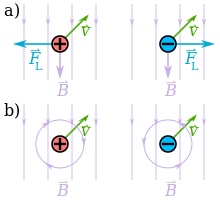
\includegraphics[width=0.45\linewidth]{pic/lorentzkraft.png}



\newpage
\subsection[Elektrostatik]{Elektrostatik\let\thefootnote\relax\footnote{}}

\concept{Punktladungen}{

\f{Ladungsdichte}{\rho(\vec r) = Q \cdot \delta(\vec r - \vec r')}\\
\f{Coulombkraft}{\vec F = \frac{1}{4\pi \varepsilon_0} \frac{q_1 q_2}{r^2}\hat{e}_r}\\
\f{elektrostatische Kraft (allg.)}{\vec F = q \vec{E}}\\
\fnote{Dipolmoment}{\vec p = q \vec d}{diskret}\\
\fnote{Dipolmoment}{\vec p = \int dV \rho(\vec r) \vec r}{kontinuierlich}\\
\fnote{Drehmoment E-Feld}{\vec{M} = \vec{p} \times \vec{E}}{el. Dipol in homogenem E-Feld}\\
\f{potentielle Energie Dipol}{W_{pot} = - \vec{p} \cdot \vec{E}}\\
\f{Kraft auf Dipol}{\vec{F} = \vec{p} \cdot \nabla \vec{E}}\\
\f{induzierter Dipol}{\vec p = \alpha \vec E}\\
\f{Quadrupolmoment}{\overleftrightarrow D = \int dV \rho(\vec r) (3 \vec r \circ \vec r - \mathbb{1} r^2)}\\
\f{Eigenschaften von $\overleftrightarrow D$}{D_{ij} = D_{ji}}\\
\f{}{\tr \overleftrightarrow D = \int dV (3 \vec r^2 - 3 \vec r^2) = 0}
}

\newpage
\concept{Makroskopische Größen}{

\f{Polarisierbarkeit}{\alpha = \frac{3\varepsilon_0}{N} \frac{\varepsilon - 1}{\varepsilon + 2}}\\
\f{Polarisation}{\vec{P} = N \vec{p}_{ind} = \varepsilon_0 \chi \vec{E}_{D}}\\
\f{Dielektrizitätskonstante}{\varepsilon = 1 + \chi = 1 + \frac{3N \alpha}{3\varepsilon_0 - N\alpha}}\\
\f{Polarisationsladungen}{\nabla \cdot \vec{P} = - \rho_{pol}}\\
\f{Potential}{\vec E = -\nabla \varphi}\\
\f{}{\varphi_{el} = \int_A \vec{E} \cdot dA}\\
\f{Laplace-Gleichung}{\Delta \varphi = 0}\\
\f{Poisson-Gleichung}{\Delta \varphi = -\frac{\rho}{\varepsilon_0}}\\
\f{Ladungsdichte}{\rho (\vec r, t) = \d{q}{V}}\\
\fnote{E-Feld von $\rho$}{E = \frac{1}{4\pi\varepsilon_0} \int_V \frac{\rho dV}{r^2}}{beliebige Ladungsdichte}\\
\f{Spannung}{U = \int_{\varphi_1}^{\varphi_2} \vec{E} \cdot d\vec{s}}\\
\f{Flächenladungsdichte}{\sigma = \frac{Q}{A}}\\
\f{Oberflächenladung}{Q = \iint \sigma dA}
}

\newpage
\concept{Kapazität}{
\fnote{Energiedichte}{w_{el} = \frac{1}{2} \varepsilon_0 E^2}{nur elektrisches Feld}\\
\f{dielektrische Verschiebungsdichte}{\vec{D} = \varepsilon \varepsilon_0 \vec{E}_{Vak} + \vec{P}}\\
\fnote{Energiedichte}{w_{el} = \frac{\varepsilon \varepsilon_0}{2} \cdot E^2 = \frac{1}{2} E \cdot D}{mit Dielektrikum}\\
\f{Ladung auf Kondensator}{Q = C U}\\
\f{E-Feld im Kondensator}{E = \frac{U}{d} = \frac{\sigma}{\varepsilon_0}}\\
\f{Energie im Kondensator}{W = \frac{1}{2} C U^2}\\
\f{Plattenkondensator}{C = \varepsilon_0 \cdot \frac{A}{d}}\\
\f{Kugelkondensator}{C = 4\pi\varepsilon_0 r}\\
\f{Zylinderkondensator}{C = \frac{2\pi\varepsilon_0 l}{\ln(r_2/r_1)}}


}

\begin{center}
\begin{framed}
	\noindent \begin{tabular}{lll}
	Geometrie & Potential $\phi$ & Feld $E$\\
	\midrule
	Punktladung & $\frac{1}{4\pi\varepsilon_0} \frac{q}{r}$ & $\frac{q}{4\pi \varepsilon_0 r^2}$\\
	Unendliche Linienladung & $\frac{1}{2\pi\varepsilon_0} \lambda \ln\frac{r_B}{r}$ & $\frac{1}{4\pi\varepsilon_0} \frac{2\lambda}{r_{\perp}}$\\
	Achse geladener Ring & $\frac{1}{4\pi\varepsilon_0} \frac{q}{\sqrt{z^2 + a^2 }}$ & $\frac{1}{4\pi\varepsilon_0} \frac{qz}{(z^2 +a^2)^{3/2}}$\\
	Kreisscheibe & $\frac{1}{2 \varepsilon_0} \sigma \abs{z} (\sqrt{1+\frac{r_S^2}{z^2}}-1)$ & $\frac{\sigma}{2 \varepsilon_0} (1-(1+\frac{r^2}{z^2})^{-1})$\\
	Unendliche Ebene & $\phi_0 - \frac{1}{2\varepsilon_0} \sigma \abs{x}$ & $\frac{\sigma}{2 \varepsilon_0}$\\
	Kugelschale & $\frac{1}{4\pi\varepsilon_0} \frac{q}{r}$ & $\frac{1}{4\pi\varepsilon_0}\frac{q}{r^2}$\\
	Dipol & $\frac{\vec p \cdot \vec r}{4\pi \varepsilon_0 r^3}$ & $\frac{1}{4\pi \varepsilon_0} \cdot \frac{3(\vec p \cdot \vec r)\vec r - \vec p r^2}{p^5}$
	\end{tabular}
\end{framed}
\end{center}

\newpage
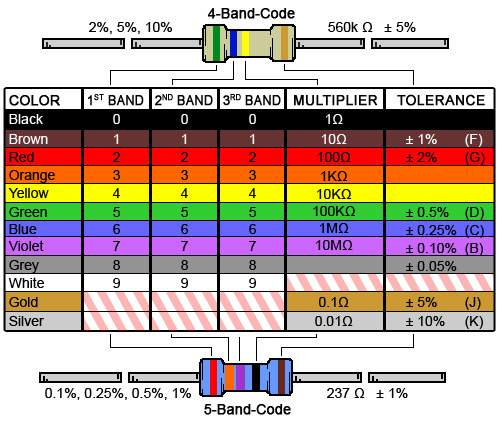
\includegraphics[width=0.9\textwidth]{pic/resistors.jpg}\\
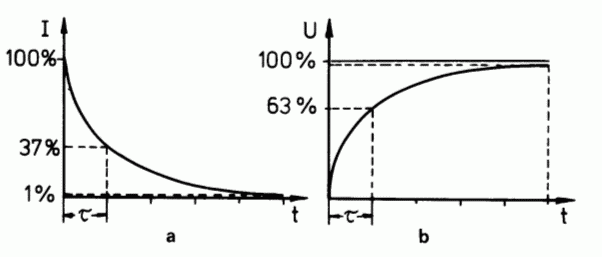
\includegraphics[width=0.9\textwidth]{pic/kondensator-aufladung.png}


\subsection[Gleichspannung]{Gleichspannung\let\thefootnote\relax\footnote{}}


\concept{Widerstand}{

\fnote{Widerstand}{R = \frac{l}{\sigma \cdot A} = \rho \frac{l}{A}}{eines Leiters}\\
\f{Flächenwiderstand}{R_S = \frac{\rho}{d} = R \frac{B}{L}}\\
\f{Leitfähigkeit}{\kappa = \frac{1}{\rho}}\\
\f{Leitwert}{G = \frac{1}{R} = \frac{I}{U}}\\
\f{Temperaturabhängigkeit}{\Delta R = R_0 \alpha \Delta T}\\
\fnote{in Serie}{R_{ges} = \sum_i R_i}{alle Ströme sind gleich groß}\\
\fnote{parallel}{\frac{1}{R_{ges}} = \sum_i \frac{1}{R_i}}{alle Spannungen sind gleich groß}\\
\f{parallel mit Leitwert}{G_{ges} = \sum_i G_i}\\
\f{zwei parellele Widerstände}{R_{ges} = \frac{R_1 \cdot R_2}{R_1 = R_2}}\\
\f{$n$ parallele, gleiche Widerstände}{R_{ges} = \frac{R}{n}}\\
\f{E12-Dekade}{10-12-15-18-22-27-33-39-47-56-68-82}\\
\f{Spannungsteiler}{\frac{U_1}{U_2} = \frac{R_1}{R_2}}

}

\begin{center}
\begin{framed}
\begin{center}
\begin{tabular}{lc}
	Ohm'sches Gesetz & $U = R \cdot I$\\
	Knotensatz & $\sum_k I_k = 0$\\
	Maschensatz & $\sum_k U_k = 0$
\end{tabular}
\end{center}
\end{framed}
\end{center}


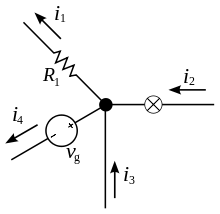
\includegraphics[width=0.45\linewidth]{pic/knotenregel.png}
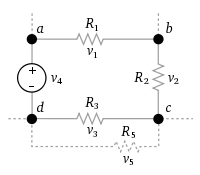
\includegraphics[width=0.45\linewidth]{pic/maschenregel.png}


\concept{Kondensator}{
\f{Kapazität}{C = \frac{Q}{U} = {I t}{U}}\\
\f{Kapazität}{C = \frac{\varepsilon_0 \varepsilon_r A}{d}}\\
\f{in Serie}{\frac{1}{C_{ges}} = \sum_i \frac{1}{C_i}}\\
\f{parallel}{C_{ges} = \sum_i C_i}\\
\fnote{Zeitkonstante}{\tau = RC}{Zeit, bis Kondensator auf 63\% aufgeladen ist}\\
\f{Verlustwiderstand}{\tan \delta = \frac{I_R}{I_C} = \frac{X_C}{R_V}}
}

\concept{Spule}{
\f{Induktivität}{L = \frac{\mu A}{l} N^2}\\
\f{in Serie}{L_{ges} = \sum_i L_i}\\
\f{parallel}{\frac{1}{L_{ges}} = \sum_i \frac{1}{L_i}}\\
\f{Güte}{Q = \frac{X_L}{R_S}}\\
\f{Verlustwiderstand}{\tan \delta = \frac{R_S}{X_L}}\\
\f{Trafoverhältnis}{\text{ü} = \frac{N_1}{N_2} = \frac{U_1}{U_2}}\\
\f{Übertrager}{\text{ü} = \sqrt{\frac{R_1}{R_2}}}
}


\conceptcon{Strom- und Spannungsquellen}{ideale Spanungsquelle: kein Innenwiderstand,
ideale Stromquelle: unendlicher Innenwiderstand}{

\fnote{Innenwiderstand reale Spannungsquelle}{R_i = \frac{\Delta U}{\Delta I}}{bei realer Spannungsquelle sackt die Spannung zusammen, wenn eine Last anliegt}\\
\fnote{Innenwiderstand lineare Stromquelle}{R_i = \frac{U_{kl}}{I_k - I}}{bei realer Stromquelle sackt die Spannung ab, wenn eine Last anliegt}

}

\concept{Leistung und Arbeit}{
\f{Leistung}{P = U I = I^2 R = \frac{U^2}{R}}\\
\f{elektrische Arbeit}{W = q U = P t = U I t}\\
\f{Wirkungsgrad}{\eta = \frac{P_{out}}{P_{in}}}

}



\subsection[Wechselspannung]{Wechselspannung\let\thefootnote\relax\footnote{}}

\concept{Grundgrößen}{
\f{komplexe Spannung}{\hat U = U e^{i \varphi_n}}\\
\f{effektive Spannung}{U_{eff} = \frac{U_{max}}{\sqrt{2}} \approx 0,707 \cdot U_{max}}

}

\concept{Komplexer Wechselstromwiderstand}{
\f{Kapazität}{X_C = \frac{U_C}{I_C} = \frac{1}{2\pi f C}}\\
\f{Induktivität}{X_L = \frac{U_L}{I_L} = 2\pi f L}\\
\f{Kapazitätsgleichung}{I_C = C \d{U_C}{t}}\\
\f{Induktivitätsgleichung}{U_L = L \d{I_L}{t}}\\
\f{Impedanz Serie}{Z = R = i X}\\
\f{Impedanz parallel}{Y = G = i B}\\
\f{Scheinleistung}{S = P + i Q}
}

\begin{center}
\begin{framed}
	\noindent
	\begin{tabular}{lll}
	L & R & C\\
	\midrule
	$\begin{array}{lcl} U_L &=& L \cdot \d{I}{t} \\ &=& \omega L I_m \cos (\omega t + \frac{\pi}{2}) \end{array}$ & $\begin{array}{lcl}U_R &=& R \cdot I \\ &=& R \cdot I_m \cos (\omega t) \end{array}$ & $\begin{array}{lcl} U_C &=& \frac{1}{C} \int I dt \\ &=& \frac{1}{\omega C} I_m \cos (\omega t - \frac{\pi}{2}) \end{array}$\\
	$X_L = \omega L$ & $R$ & $X_C = \frac{1}{\omega C}$\\
	$\varphi = +\frac{\pi}{2}$ & $\varphi = 0$ & $\varphi = -\frac{\pi}{2}$\\
	$I$ zu spät & gleichphasig & $I$ eilt vor\\
	\end{tabular}
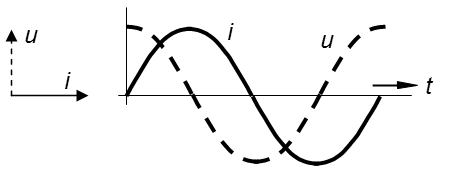
\includegraphics[width=0.45\linewidth]{pic/spule-strom.png}
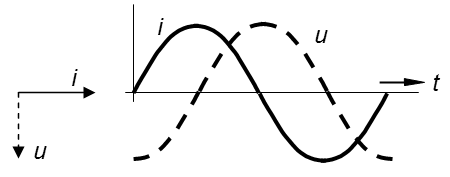
\includegraphics[width=0.45\linewidth]{pic/kondensator-strom.png}
\end{framed}
\end{center}


\concept{Schwingkreis}{
\f{Resonanzfrequenz}{f_0 = \frac{1}{2\pi \sqrt{LC}}}\\
\f{Wellengleichung}{\ddot{I} + \frac{R}{L} \dot{I} + \frac{1}{LC} I = f(t)}\\
\f{Güte Reihenschwingkreis}{Q = \frac{X_L}{R_S}}\\
\f{Güte Parallelschwingkreis}{Q = \frac{R_P}{X_L}}\\
\f{Bandbreite}{B = \frac{f_0}{Q}}
}




\begin{center}
\begin{framed}
\begin{tabular}{lcc}
Schwingkreis/Filter & Impedanz bei $f$ & Verhalten\\
\midrule
Saugkreis & klein bei $f_{res}$ & wird Kurzschluss\\
Sperrkreis & groß bei $f_{res}$ & wird hochohmig\\
Tiefpass & klein bei kleinen $f$ & lässt kleine Frequenzen durch\\
Hochpass & klein bei großen $f$ & lässt hohe Frequenzen durch
\end{tabular}


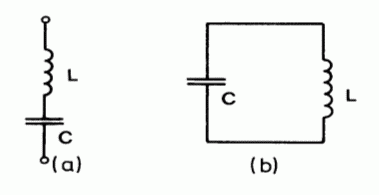
\includegraphics[width=0.45\linewidth]{pic/schwingkreis.png}
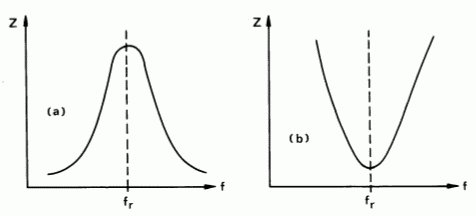
\includegraphics[width=0.45\linewidth]{pic/schwingkreis-antwort.png}
\end{framed}
\end{center}


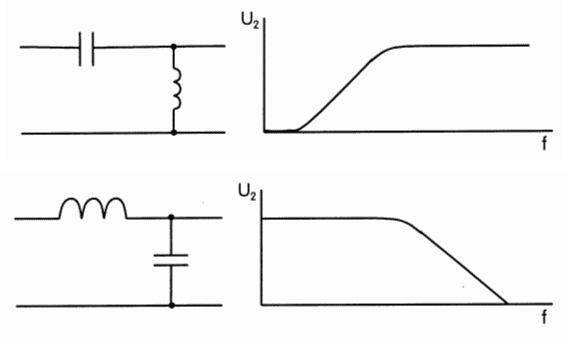
\includegraphics[width=0.45\linewidth]{pic/hochtiefpass.png}
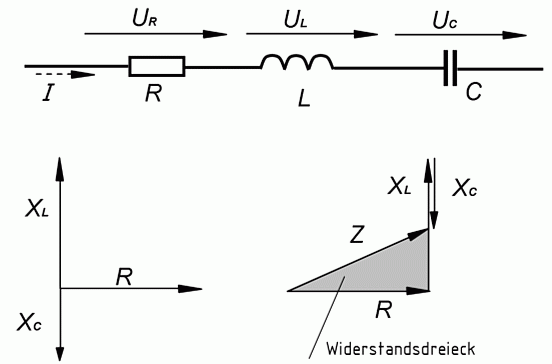
\includegraphics[width=0.45\linewidth]{pic/rlc.png}\\

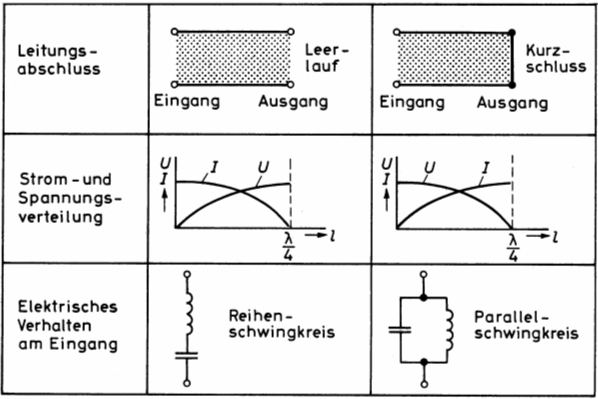
\includegraphics[width=0.9\linewidth]{pic/lecherleitung.png}


\concept{Gleichrichtung}{

}

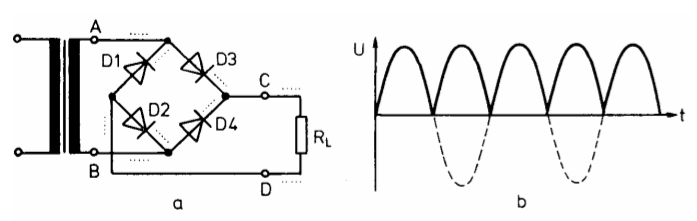
\includegraphics[width=\linewidth]{pic/fbr.png}\\
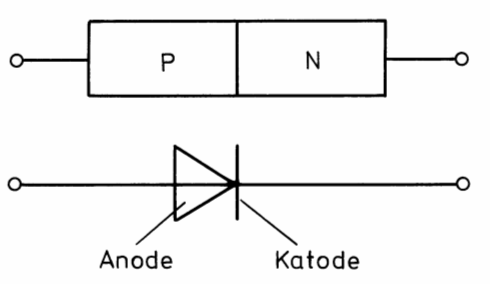
\includegraphics[width=0.55\linewidth]{pic/pn-ak.png}
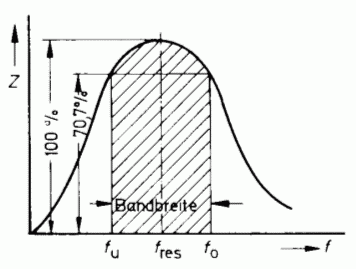
\includegraphics[width=0.40\linewidth]{pic/bandbreite.png}



\subsection[Leitungstheorie]{Leitungstheorie\let\thefootnote\relax\footnote{}}

\begin{center}
\begin{framed}
$$\pdd{I}{x} - \rho l \pdd{I}{t} - (\rho r + gl) \pd{I}{t} - grI = 0$$
\centering Telegraphengleichung
\end{framed}
\end{center}

\concept{Leitungstheorie}{
\f{Leiterschleife}{\dot U_i = R_i \dot I_i + \frac{I_i}{C_i} + \sum_k L_{ik} \ddot I_k}\\
\f{Leistung}{N = U I = RI^2 + \d{}{t} (\frac{1}{2} LI^2 + \frac{1}{2} \frac{Q^2}{C})}\\
\f{Drahtwelle}{\pd{u}{x} + rI +l \dot I = 0}\\
\f{Ladungsbilanz}{\rho \dot U + \pd{I}{x} + gU = 0}\\
\f{Wellenwiderstand}{U = \pm l v_0 I = \pm \sqrt{\frac{l}{\rho}} I}\\
\f{ideale Leitung}{v_0^2 = \frac{1}{\rho l}}\\
\f{nicht-ideale Leitung}{\Delta \Vec E - \mu \sigma \dot{\vec{E}} = 0$, $\Delta \js - \mu \sigma \dot \js = 0}\\
\f{Wellenwiderstand bei Skin-Effekt}{Z = \frac{El}{I}}\\
\f{Wechselstromwiderstand}{\frac{Z}{l} = \frac{(1-i) k_0}{2\pi r \sigma} = \frac{1-i}{2\pi r} \sqrt{\frac{\mu \omega}{2 \sigma}}}
}

\concept{Reale Leitungen}{
\f{Paralleldrahtleitung}{Z = \frac{120~\Omega}{\sqrt{\varepsilon_r}} \ln \Big(\frac{2a}{d}\Big)}\\
\f{Koaxialleitung}{Z = \frac{60~\Omega}{\sqrt{\varepsilon_r}} \ln \Big(\frac{D}{d}\Big)}\\
\f{Ausbreitungsgeschwindigkeit}{v = \frac{1}{\sqrt{L' C'}}}\\
\f{Verkürzungsfaktor}{k = \frac{v}{c} = \frac{1}{\sqrt{\varepsilon_r}}}\\
\fnote{Wellenwiderstand}{Z = \sqrt{Z_1 Z_2}}{zur Anpassung mittels Transformationsleitung}\\
\f{Länge Transformationsleitung}{l = (2n-1) \frac{\lambda}{4}k}
}

\concept{Praktische Kenngrößen}{
\f{Dämpfungsfaktor}{D = \frac{P_1}{P_2}}\\
\f{Dämpfungsmaß (Leistung)}{a_P = 10 \cdot \log \frac{P_1}{P_2}}\\
\f{Dämpfungsmaß (Spannung)}{a_U = 20 \cdot \log \frac{U_1}{U_2}}\\
\f{Wellenwiderstand}{Z = \sqrt{\frac{L'}{C'}}}\\
\f{VSWR}{VSWR = \frac{U_{max}}{U_{min}}}\\
\f{Leistungspegel}{p = 10 \cdot \log \frac{P}{1\text{mW}} \text{dBm}}
\f{reflektierte Leistung}{P_r = P_v \Big(\frac{s-1}{s+1}\Big)^2}\\
\f{SWR}{SWR = \frac{R_a}{Z} \text{ oder } \frac{Z}{R_a}}\\

}

\begin{center}
\begin{framed}
\begin{center}
\begin{tabular}{c|ccccccccc}
& S9 & S8 & S7 & S6 & S5 & S4 & S3 & S2 & S1\\
\midrule
KW & 50 & 25 & 12,5 & 6,25 & 3,12 & 1,56 & 0,78 & 0,39 & 0,2\\
UKW & 5 & 2,5 & 1,25 & 0,62 & 0,31 & 0,16 & 0,08 & 0,04 & 0,02
\end{tabular}
\end{center}
\end{framed}
\end{center}


\subsection[Antennentechnik]{Antennentechnik\let\thefootnote\relax\footnote{}}

\concept{Kenngrößen}{
\f{Eingangsimpedanz}{Z = \frac{U}{I}}\\
\f{EIRP}{P_{EIRP} = (P_{Sender} - P_{Verluste}) \cdot G_{isotrop}}\\
\f{ERP}{P_{ERP} = (P_{Sender} - P_{Verluste}) \cdot G_{Dipol}}\\
\f{Verhältnis ERP und EIRP}{P_{EIRP} = 1.64 P_{ERP}}\\
\f{Feldstärke Fernfeld}{E = \frac{\sqrt{30~\Omega P_{EIRP}}}{r}}\\
\f{Sicherheitsabstand}{r = \frac{\sqrt{30 P_{EIRP}\text{[W]}}}{E\text{[V/m]}}}\\

}

\concept{Dimensionierung}{
\f{Frequenz}{f\text{[MHz]} = \frac{300}{\lambda\text{[m]}}}\\
\f{Verkürzungsfaktor}{k = \frac{l}{\lambda/2} \approx 0,95}\\

}

\concept{Wellenausbreitung}{
\fnote{MUF}{MUF = \frac{f_k}{\sin \alpha}}{maximum usable frequency}\\
\f{optimale Frequenz}{f_{opt} = 0,85 \cdot MUF}\\
\f{Feldwellenwiderstand}{Z = \frac{E}{H} = \sqrt{\frac{\mu_0}{\varepsilon_0}} \approx 120\pi~\Omega = 377~\Omega}
}

\subsection[Signale]{Signale\let\thefootnote\relax\footnote{}}

\concept{Amplitudenmodulation}{
\f{Modulationsgrad}{m = \frac{\hat U_{mod}}{\hat U_T}}\\
\f{Bandbreite}{B = 2 f_{mod max}}\\

}

\concept{Frequenzmodulation}{
\f{Modulationsindex}{m = \frac{\Delta f_T}{f_{mod}}}\\
\f{Carson-Bandbreite}{B = 2 (\Delta f_T + f_{mod max})}\\

}

\subsection{Plasmonik}

\concept{Drude- und Lorentzmodell}{
\f{Permittivität}{\varepsilon = 1 - \frac{\omega_p^2}{\omega^2 + i \gamma \omega}}\\
\f{Dämpfung}{\eps' = \frac{\omega_p^2 \gamma}{\omega(\omega^2 + \gamma^2)}}\\
\f{Stromdichte}{\js =\frac{n \cdot q^2 \cdot \tau_s}{m} \vec{E}}\\
\f{Geschwindigkeit}{v = \frac{q}{m} \tau E}\\
\f{Driftgeschwindigkeit}{\vec{v}_D = \frac{q \cdot \tau}{m} \cdot \vec{E} = \frac{\sigma}{n \cdot q} \cdot \vec{E}}\\
\f{Plasmafrequenz}{\omega_p^2 = \frac{N e^2}{\varepsilon_0 m}}\\
\f{Absorptionskoeffizient}{\alpha(\omega) = \frac{2\omega}{c}k(\omega)}\\
\f{Skin Depth}{d = 1/\alpha}
}

\concept{Plasmonen}{
\f{Volumenplasmon}{\eps = 0$, $\omega = \omega_p}\\
\f{Flächenplasmon}{\eps = -1$, $\omega = \frac{\omega_p}{\sqrt{2}}}\\
\f{Lokalisiertes Plasmon}{\eps = -2$, $\omega = \frac{\omega_p}{\sqrt{3}}}\\
}


\subsection[Magnetostatik]{Magnetostatik\let\thefootnote\relax\footnote{}}

\concept{Magnetische Dipole}{

\f{mag. Dipolmoment}{\vec{\mu}_m = I \cdot \vec{A} = \frac{q}{2m} \cdot \vec{L}}\\
\f{Feld eines Dipols}{\vec B = \frac{\mu_0}{4\pi} \frac{1}{r^5} 3(\vec m \cdot \ort)\ort - mr^2}\\
\f{Vektorpotential}{\vec A (\ort) = \frac{\mu_0 I}{4\pi} \vec A_r \times \frac{\ort}{r^3} = \frac{\mu_0}{4\pi} \frac{\vec m \times \vec r}{r^3}}\\
\f{Drehmoment im B-Feld}{\vec{M} = \vec{\mu}_m \times \vec{B}}\\
\f{potentielle Energie Dipol}{E_{pot} = -\vec{\mu}_m \cdot \vec{B}}\\
\f{Bohr'sches Magneton}{\mu_B = \frac{e \cdot \hbar}{2 m_e}}\\
\f{Ladung auf Umlaufbahn}{\vec m = I \cdot \vec A_p = \frac{1}{2} \frac{Q}{m} \vec L}\\
\f{Dipolmoment allg. Stromverteilung}{\vec m = \frac{1}{2} \int dV \ort \times \vec \jmath (\ort)}\\

}

\concept{Magnetfeld}{

\f{Biot-Savart}{\vec{B} = -\frac{\mu_0 I}{4\pi} \int \frac{d\vec{l}\times\vec{r}}{r^2}}\\
\f{Vektorpotential}{\vec B = \nabla \times \vec A}\\
\f{Coulomb-Eichung}{\nabla \cdot \vec A = 0}\\
\f{Flussdichte}{-\Delta \vec A = \mu_0 \vec \jmath}\\
\f{magnetischer Fluss}{\phi_m = \int_A \vec{B} \cdot d\vec{A}}\\
\f{allg. Vektorpotential}{\vec A (\vec r) = \frac{\mu_0}{4\pi} \int \frac{dV' \vec \jmath (\vec r')}{\abs{ \vec r - \vec r'}}}\\
\f{allg. Flussdichte}{\vec B (\vec r) = \frac{\mu_0}{4\pi} \int \frac{dV' \vec \jmath (\vec r) \times (\vec r - \vec r')}{\abs{\vec r - \vec r'}^3}}\\

}

\concept{Induktion}{
\f{Induktivität}{L_{ik} = \frac{\mu_0}{4\pi} \oint d\vec r \oint d\vec r' \frac{1}{\rd}}\\
\f{Selbstinduktivität}{L_{ik} = L_{ki}}\\
\f{Selbstinduktivität Zylinder}{L = \mu_0 (\frac{n}{l})^2 A l}\\
\f{Kraft auf Leiterelement}{d\vec{F} = I \cdot (d\vec{l} \times \vec{B})}\\
\f{Kraft auf Leiter}{\vec F = \vec B I l}\\
\f{Hall-Spannung}{U_H = \vec{b} \cdot \vec{E}_H = \frac{I \cdot B}{n \cdot e \cdot d} = R_H \frac{B}{b} I}\\
\f{Zyklotron}{\frac{q}{m} v B = \frac{v^2}{r}}\\
\f{Selbstinduktion}{\phi_m = L I}\\
\f{Induktionsspannung}{U_{ind} = - L \dot{I} =  v B l}\\
\f{Energie im mag. Feld}{W_{mag} = \frac{1}{2} L I^2}\\
\f{Gegeninduktion}{L = \frac{\phi_{12}}{I_1} = \frac{\phi_{21}}{I_2}}\\
\f{Energiedichte}{w_{mag} = \frac{1}{2} \mu_0 H^2 = \frac{1}{2 \mu}B^2}\\
\f{Curie-Gesetz}{C = \kappa T}
}

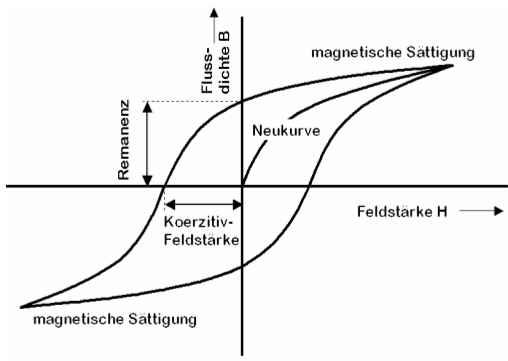
\includegraphics[width=0.9\linewidth]{pic/magnetisierung.png}

\begin{center}
\begin{framed}
	\begin{tabular}{lll}
	Geometrie & $\phi$ & $E$\\
	\midrule
	Leiter & $\frac{\mu_0 I}{2\pi r}$ & \\
	Schleife (z-Achse) & $\frac{\mu_0}{4\pi}\frac{2\pi r^2 I}{(z^2 + r^2)^{3/2}}$ & \\
	Schleife & $\frac{\mu_0}{4\pi} \sum_n I_n \int \frac{d\vec r' \times \abs{\vec r - \vec r'}}{\abs{\vec r- \vec r'}^3}$ & \\
	lange Spule & $\frac{\mu_0 n I}{l}$ & \\
	dichte Spule & $\frac{\mu_0}{2\pi}\frac{n I}{r}$ & \\
	\end{tabular}
\end{framed}
\end{center}

\subsection{Elektromagnetische Wellen}

\begin{center}
\begin{framed}
$$\Big(\frac{1}{c^2} \pdd{}{t} - \Delta\Big) \vec E = \square \vec E = 0$$
$$\hat k \times \vec E = c \vec B$$
\centering Wellengleichung
\end{framed}
\end{center}

\concept{Wellen im Freiraum}{
\f{vollständige Lösung}{u = u_1 (x-ct) + u_2 (x+ct)}\\
\f{Dispersion Vakuum}{\omega^2 = c^2 \vec k^2}\\
\f{Phasengeschwindigkeit}{v_{ph} = \frac{\omega}{k}}\\
\f{Gruppengeschwindigkeit}{v_{gr} = \pd{\omega}{k}}\\
\f{ebene Welle}{\vec E = \vec E_0 e^{i(\vec k \cdot \ort - \omega t)}}\\
\f{elliptisch polarisiert}{\vec E_0 = \vec E_1 + i \vec E_2}
}



\subsection[Energie und Impuls im EM-Feld]{Energie und Impuls im EM-Feld\let\thefootnote\relax\footnote{}}

\concept{Energie}{

\f{Energiedichte}{w_{em} = \frac{1}{2}(E D + B H)}\\
\f{Poynting-Vektor}{\vec S = \frac{1}{\mu_0} (\vec E \times \vec B)}\\
\f{Änderung der Energiedichte}{\nu_{em} = - \js \cdot \vec E}\\
\f{Poynting-Theorem}{\pd{w}{t} + \nabla \cdot \vec S = - \js \cdot \vec E}\\
\f{Energie}{W_{em} = \frac{1}{2} \int dV \rho \varphi}\\
\f{allg. Ohm'sches Gesetz}{\js = \sigma \vec E}\\
\f{Thomson'scher Satz}{W_c \text{ nimmt im GG Extr. an}}\\
\f{Energie Magnetfeld}{W_m = \frac{1}{2} \sum_i I_i \Phi_i}\\
\f{Selbstenergie}{W_m = \frac{1}{I^2} \int dV \frac{\vec B^2}{\mu_o} = \frac{\Phi}{I}}\\
\f{Energiestromdichte Welle}{\vec S_p = c \hat k \omega}\\
\f{Imulsbilanz}{\pd{\vec g}{t} + \nabla \cdot \overleftrightarrow T = - \vec f_L}\\
\f{Impulsdichte}{\vec g = \varepsilon_0 (\vec E \times \vec B)}\\
\f{Kraftdichte}{\vec f_l = \rho \vec E + \js \times \vec B}\\
\f{Strahlungsdruck}{P = \frac{w}{3}}\\
\f{mittlere Leistung Hertz'scher Dipol}{\bar{P}_{em} = \frac{p^2}{12\pi \varepsilon_0 \varepsilon c^3} \omega^4}\\
\f{Magnetfeldvektor}{\vec{B}_0 = \frac{1}{\omega} (\vec{k} \times \vec{E}_0) = \frac{1}{c} (\vec{e}_k \times \vec{E}_0)}\\
\f{anisotropes Medium}{\vec D = \varepsilon_0 (1+\chi) \vec E}

}


\subsection[Zeitabhängige Felder]{Zeitabhängige Felder\let\thefootnote\relax\footnote{}}

\concept{Abstrahlung}{
\f{Stromdichte}{\vec J(t) = \int dV \js (\ort, t) = \dot{\vec{p}}}\\
\f{Fernfeld}{\vec E(\ort, t) = c \vec B \times \vec n}\\
\f{Energieabstrahlung hD}{\abs{\vec S_p} = \frac{\mu_0}{16\pi^2c} \frac{1}{r^2} (\ddot{\vec{p}}^2 \sin^2 \vartheta)}\\
\f{Zeitmittel abgestrahlte Leistung}{\bar N = \frac{\mu_0 \omega^2 \vec p_0^2}{12 \pi c}}\\
\f{Energieabstrahlung}{\vec S_p = \hat n \frac{\mu_0}{16\pi^2 c} \frac{(\ddot{\vec{q}} \times \hat n)^2}{r^2}}\\
\f{Strahlungsbremskraft}{\vec F_s = \frac{Q^2}{4\pi c^3 \varepsilon_0} \ddot{\vec{R}}}


}

\subsection[EM-Felder in Substanzen]{EM-Felder in Substanzen\let\thefootnote\relax\footnote{}}


\concept{Felder in Substanzen}{

\f{Polarisation}{\vec P = \chi_e \varepsilon_0 \vec E}\\
\f{Magnetisierung}{\vec M = \chi_m' \frac{1}{\mu_0} \vec B}\\
\f{Verschiebungsdichte}{\vec D = \varepsilon_0 \varepsilon_r \vec E = \varepsilon \vec E = (1+\chi_e) \varepsilon_0 \vec E}\\
\f{Magnetfeld}{\vec H = (1-\chi_m') \frac{1}{\mu_0} \vec B}\\
\f{Flussdichte}{\vec B = \frac{\mu_0}{1-\chi_m'} \vec H}\\
\f{Ströme}{\js = \js_k + \js_L + \js_P + \js_M}\\
\f{Magnetisierungsstrom}{\js_M = \nabla \times \vec M}\\
\f{Impulsdichte}{\vec g = \vec D \times \vec B = \frac{n^2}{c_0^2} \vec S_p}\\
\f{Clausius-Mosotti}{\abs{\frac{\varepsilon_r - 1}{\varepsilon_r + 2}} = \frac{\kappa}{3}}

}

\concept{Supraleiter}{

\f{Eigenschaften}{\sigma = \infty, \vec B = 0}\\
\f{1. London-Gleichung}{\pd{\js_s}{t} = \frac{n_s* \cdot e*^2}{m*} \vec E}\\
\f{2. London-Gleichung}{\nabla \times \js_S + \frac{n_s* \cdot e*^2}{m*} \vec B = 0}
}

\begin{center}
\begin{framed}
\begin{align*}
\nabla \cdot \vec D &= \rho_{\text{frei}}\\
\nabla \cdot \vec B &= 0\\
\nabla \times \vec E &= - \pd{\vec{B}}{t}\\
\nabla \times \vec H &=  \mu_0 \vec \jmath_{\text{frei}} + \pd{\vec{D}}{t}\\
\vec D &= \varepsilon_0 \vec E + \vec P\\
\vec H &= \frac{1}{\mu_0} \vec B - \vec M\\
\hat n (\vec{D_2} - \vec{D_1}) &= \sigma_o\\
\hat n (\vec{B_2} - \vec{B_1}) &= 0\\
\hat n \times (\vec{E_2} - \vec{E_1}) &= 0\\
\hat n \times (\vec{H_2} - \vec{H_1}) &= \vec k\\
\end{align*}
\end{framed}
\end{center}


\newpage
\section{Optik}

\subsection[Wärmestrahlung]{Wärmestrahlung\let\thefootnote\relax\footnote{}}

\concept{Schwarzer Körper}{
\f{Strahlungsgesetz}{S = \sigma T^4}\\
\f{Wien'sches Verschiebungsgesetz}{\lambda_{max} T = 2,898~\text{mmK}}\\
\f{Planck'sches Strahlungsgesetz}{W(\lambda, T)  = \frac{hc^3}{\lambda^5 \exp{(hc/ \lambda k_B T)} - 1}}\\
\f{Boltzmann-Verteilung}{P_n = \frac{\exp{- \beta E_n}}{\sum_n \exp{-\beta E_n}}}\\
\f{Teilchenzahl}{\erw{n} = \frac{1}{\exp{\beta \hbar \omega} - 1}}\\
\f{Dichteoperator}{\hat \rho = \sum_n \frac{\erw{n}^n}{(1+\erw{n})^{1+n}} \ket n \bra n}
}

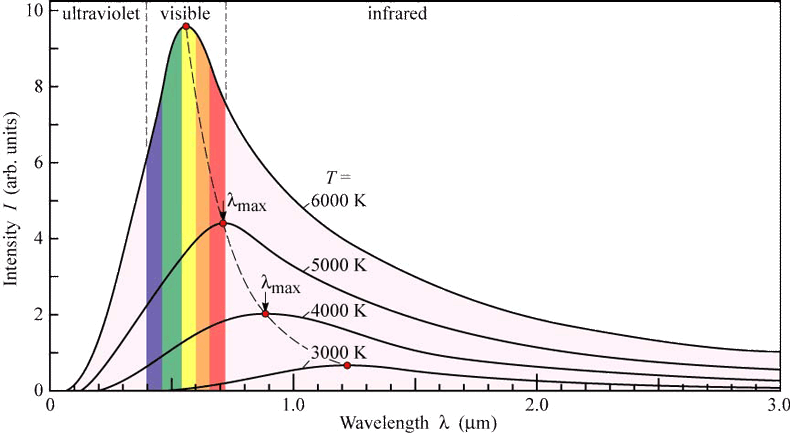
\includegraphics[width=\linewidth]{pic/planck.png}\\
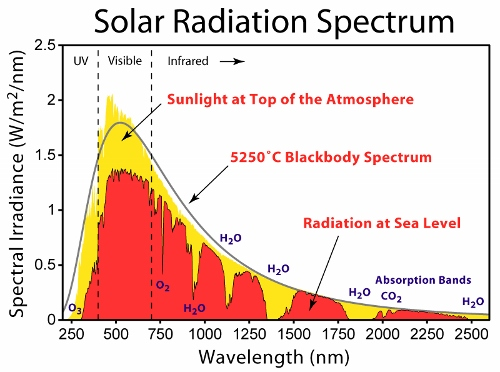
\includegraphics[width=\linewidth]{pic/sonnenspektrum.jpg}\\

\subsection[Strahlenoptik]{Strahlenoptik\let\thefootnote\relax\footnote{$\eps_r$: relative Permittivität im Medium, $\mu_r$: relative Permeabilität im Medium, $d$: Länge, $\alpha$: Einfalls-/Austrittswinkel, $g$: Gegenstandsweite, $b$: Bildweite, $f$: Brennweite, $r$: Krümmungsradius, $d$: Linsendicke, $M$: Mittelpunktsstrahl, $P$: Parallelstrahl, $B$: Brennstrahl}}

\concept{Komplexer Brechungsindex}{
\f{Brechungsindex}{n = \frac{c}{v} = \sqrt{\varepsilon_r \mu_r}}\\
\f{optische Pfadlänge}{\Delta = nd = ct}\\
\f{Reflexionsgesetz}{\alpha_1 = \alpha_2}\\
\f{Brechungsgesetz}{n_1 \sin \alpha_1 = n_2 \sin \alpha_2}\\
\f{Strahlverengung}{\Delta b = \frac{\cos \alpha_2}{\cos \alpha_1}}\\
\f{kritischer Winkel}{\sin \alpha_C = \frac{n_1}{n_2}}\\
\f{Brewster-Winkel}{\tan \alpha_B = \frac{n_2}{n_1}}\\
\f{Abweichung}{\frac{n_2}{n_1} = \frac{\sin \frac{1}{2}(\alpha + \delta_m)}{\sin \frac{1}{2} \alpha}}
}

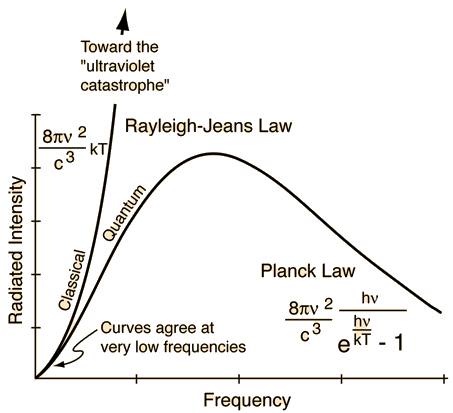
\includegraphics[width=0.45\linewidth]{pic/rj.png}
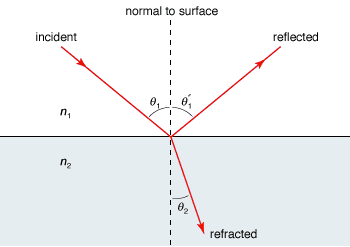
\includegraphics[width=0.45\linewidth]{pic/snellius.png}\\
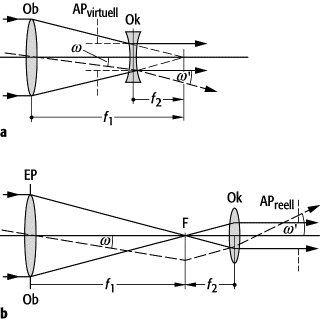
\includegraphics[width=0.45\linewidth]{pic/teleskop.jpg}
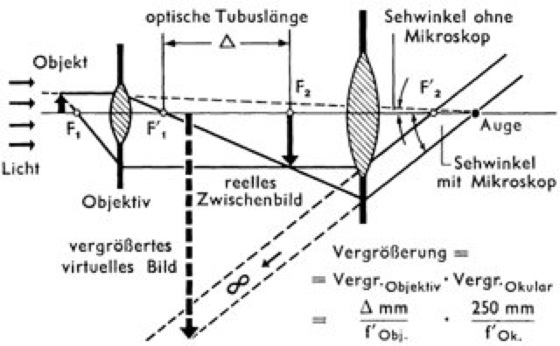
\includegraphics[width=0.45\linewidth]{pic/mikroskop.jpg}

\concept{Abbildungen}{
\f{dünnes Prisma}{\frac{n_2}{n_1} = \frac{\alpha + \delta_m}{\alpha}}\\
\f{Gauss'sche Formel}{\frac{n_1}{g} + \frac{n_2}{b} = \frac{n_2 - n_1}{r}}\\
\f{Linsengleichung}{\frac{1}{g} + \frac{1}{b} = \frac{1}{f}}\\
\f{Linsenschleiferformel}{\frac{1}{f} = (n-1) (\frac{1}{r_1} - \frac{1}{r_2} + \frac{(n-1)d}{n r_1 r_2})}\\
\f{Strahlengang}{\text{M} \rightarrow \text{M}, \text{P} \leftrightarrow \text{B}}\\
\f{Vergrößerung}{V = \frac{B}{G} = -\frac{b}{g}}\\
\f{Dioptrie}{P = 1/f[\text{m}]}\\
\f{Vergrößerung Linse}{V_L = \frac{s_0}{f} = \frac{\sigma}{\sigma_0}}\\
\f{Vergrößerung Mikroskop}{V_M = V_{Ob} V_{Ok} = -\frac{l}{f_{Ob}} \frac{s_0}{f_{Ok}}}\\
\f{Vergrößerung Teleskop}{V_T = -\frac{f_{Ob}}{f_{Ok}}}\\
\f{Spiegelgleichung}{\frac{1}{f} = -\frac{2}{r}}\\
\f{Astigmatismus-Positionen}{\frac{1}{g} + \frac{1}{i_T} = -\frac{2}{r \cos \alpha}}\\
\f{}{\frac{1}{g} + \frac{1}{i_S} = -\frac{2 \cos \alpha}{r}}
}


\subsection[Elektromagnetische Wellen]{Elektromagnetische Wellen\let\thefootnote\relax\footnote{}}

\concept{Grundgrößen}{
\f{Phase}{\omega t - k x}\\
\f{Phasengeschwindigkeit}{v_{ph} = \frac{\omega}{k}}\\
\fnote{Dopplereffekt}{f' = f(1+\frac{v}{c})}{nicht relativistisch}\\
\f{Gruppengeschwindigkeit}{v_{gr} = \pd{\omega}{k}}\\
\f{Wellenvektor}{\vec k = \frac{2 \pi}{\lambda} \hat e}\\
\f{Poynting-Vektor}{\vec{S} = \frac{1}{\mu_0}(\vec{E} \times \vec{B})}\\
\f{Strahlungsdruck}{p_S = I/c}\\
\f{Intensität}{I = \frac{P}{A} = |\vec{S}|}\\
\f{Impuls}{p = \frac{W}{c}}\\
\f{Wellengleichung}{\nabla^2 \vec E - \frac{1}{c^2} \ddot{\vec{E}} = \square \vec E = 0}\\
\f{ebene monochromatische Welle}{\vec E = \vec E_0 \exp [\iu(\vec k \ort - \omega t + \varphi)]}\\

}

\begin{center}
\begin{framed}
$$c = \frac{1}{\sqrt{\varepsilon_0 \mu_0}} = \frac{\omega}{k} = \lambda \cdot f$$
$$k = \frac{2\pi}{\lambda}$$
$$\omega = 2\pi f = \frac{2\pi}{T}$$
\end{framed}
\end{center}

\begin{center}
\begin{framed}
$D_{n,1} = D_{n,2}$, $E_{t,1} = E_{t,2}$\\
$B_{n,1} = B_{n,2}$, $H_{t,1} = H_{t,2}$\\
Grenzflächenbedingungen
\end{framed}
\end{center}

\subsection[Interferenz]{Interferenz\let\thefootnote\relax\footnote{}}

\concept{Doppelspalt}{
\f{konstruktiv}{x = m \lambda \frac{D}{d}}\\
\f{destruktiv}{x = (m+ \frac{1}{2}) \lambda \frac{D}{d}}
}

\concept{Fresnel'sches Biprisma}{
\f{Wellenlänge}{\lambda = \frac{\Delta x d}{B + C}}
}

\concept{Interferenz}{
\f{Gesamtintensität}{I = I_1 + I_2 + 2\sqrt{I_1 I_2} \cos \theta}\\
\f{Michelson-Interferometer}{I = 1+\cos \theta = 1+\cos(\frac{2\pi d}{\lambda})}\\
\f{Zeitmittel}{\langle f(t) \rangle = \lim_{T \rightarrow \infty} \frac{1}{T} \int_0^T f(t) dt}\\
}

\begin{center}
\begin{framed}
Die Emission aus einer flächigen Quelle und die daraus resultierende Überlagerung an zwei Raumpunkten $P_1$ und $P_2$ kann als Beugungs- bzw. Streuproblem behandelt werden.\\
\centering\textsc{Van Cittert-Zernike-Theorem}
\end{framed}
\end{center}

\subsection[Beugung und Dispersion]{Beugung und Dispersion\let\thefootnote\relax\footnote{}}

\concept{Beugung}{
\f{langer Spalt}{I = A_0^2 \frac{\sin^2 \beta}{\beta^2}}\\
\f{}{\beta = \frac{1}{2}kb\sin \Theta}\\
\f{}{A_0 = \frac{ab}{x}}\\
\f{Einfall unter $i$}{\beta = \frac{b \pi (\sin i + \sin \Theta)}{\lambda}}\\
\f{rechteckiger Spalt}{I \sim b^2 l^2 \frac{\sin^2 \beta}{\beta^2} \frac{\sin^2 \gamma}{\gamma^2}}\\
\fnote{Rayleigh-Kriterium}{\Theta = \frac{\lambda}{b}}{rechteckige Apertur}\\
\fnote{Rayleigh-Kriterium}{\Theta = 1.22 \frac{\lambda}{D}}{runde Apertur}\\
\f{Beugungsgitter}{d(\sin i + \sin \Theta) = m \lambda}\\

}

\concept{Dispersion}{
\f{Winkeldispersion}{\frac{\Delta \Theta}{\Delta \lambda} = \frac{m}{d \cos \Theta}}\\
\f{Gitterauflösung}{\Delta \Theta = \frac{\lambda}{N d \cos \Theta}}\\
\f{Resolving Power}{RP = \frac{\omega}{\delta \omega} = \frac{\nu}{\delta \nu} = \frac{\lambda}{\delta \lambda}}\\
\f{Fresnel}{R_n = \sqrt{n \lambda L}}\\
\f{Fesnel-Zone Fläche}{A = \pi \lambda L}\\
\fnote{fokale Länge}{l = \frac{R_1^2}{\lambda}}{Fresnellinse}
}


\subsection[Leiteroperatoren und kohärente Zustände]{Leiteroperatoren und kohärente Zustände\let\thefootnote\relax\footnote{}}

\concept{Kohärente Zustände}{
\f{Vernichtungsoperator}{\hat a \psi_n = \sqrt n \psi_{n-1}}\\
\f{Vernichtungsoperator}{\hat a = \frac{1}{\sqrt{2}} (\xi + \d{}{\xi})}\\
\f{Erzeugungsoperator}{\hat a^\dagger \psi_n = \sqrt{n-1} \psi_{n-1}}\\
\f{Erzeugungsoperator}{hat a^\dagger = \frac{1}{\sqrt{2}} (\xi - \d{}{\xi})}\\
\f{Kommutator}{[a, a^\dagger] = 1}\\
\f{Teilchenzahloperator}{\hat N = a^\dagger a = \hat N^\dagger}\\
\f{Identität}{a a^\dagger - a^\dagger a = 1}\\
\fnote{Hamiltonian}{\hbar \omega (a^\dagger a + 1/2)}{harmonischer Oszillator}\\
\f{auf Teilchenzahlzustand}{\hat a \ket n = \sqrt{n} \ket{n-1}}\\
\f{}{\hat a^\dagger \ket n = \sqrt{n+1} \ket{n+1}}\\
\f{Vakuumzustand}{\hat a \ket 0 = 0}\\
\f{Quantisierung EM-Feld}{\vec A_k = \sqrt{\frac{\hbar}{2 \varepsilon_0 V \omega_k}} \hat a_k \vec e_k}\\
\f{}{\vec A_k^* = \sqrt{\frac{\hbar}{2 \varepsilon_0 V \omega_k}} \hat a_k^\dagger \vec e_k}\\
}

\subsection[Kohärenz]{Kohärenz\let\thefootnote\relax\footnote{}}

\concept{Kohärenz}{
\f{Gesamtintensität}{I = I_1 + I_2 + 2 \sqrt{I_1 I_2} \Re[k_1 k_2 \gamma^1 (x_1, x_2)]}\\
\f{Korrelationsfunktion}{\Gamma_{12}(\tau) = \Re \{ \frac{1}{T} \int_0^T \vec E_1(t) \cdot \vec E_2^*(t + \tau) dt}\\
\f{Lorentzpuls}{\gamma^{(1)} = \exp{-i \omega_0 \tau} \exp{-\abs{\tau} / \tau_c}}\\
\f{Gaußpuls}{\gamma^{(1)} = \exp{-i \omega_0 \tau} \exp{-\frac{\pi}{2} (\frac{\tau}{\tau_c})^2}, \tau_c = \frac{\sqrt{8 \pi \ln 2}}{\Delta \omega}}\\
\f{Kohärenzlänge}{l_c = c \langle \tau_0 \rangle = \frac{c}{\Delta \nu}}\\
\f{Frequenzbandbreite}{\Delta \omega = \frac{2\pi}{\tau_0}}\\
\f{Linienbreite}{\Delta \lambda = \frac{\lambda_0^2}{l_c}}\\
\fnote{Kohärenzlänge}{l_t = \frac{\lambda r}{s} = \frac{\lambda}{\theta_s}}{$\theta_s$ Winkelauflösung}\\
\f{$l_t$ runde Quelle}{l_t = \frac{1,22 \lambda}{\theta_s}}\\
\f{Kontrast}{V = \frac{I_{max} - I_{min}}{I_{max} + I_{min}} = \frac{2\sqrt{I_1 I_2} \cdot \abs{\gamma^1}}{I_1 + I_2}}\\
\f{Kontrast (gleiche Amplitude)}{V = \abs{\gamma_{12}}}\\
\f{Kohärenz 2. Ordnung}{\gamma^{2}(\tau) = \frac{\erw{I(t) I(t+\tau)}}{\erw{I(t)}^2}}

}

\subsection[Optische Elemente]{Optische Elemente\let\thefootnote\relax\footnote{}}

\concept{Elemente}{
\f{Phasenplatte}{H = \hbar (\omega + \phi) \hat a^\dagger \hat a}\\
\f{eff. Phasenverschiebung}{\phi t = \varphi}\\
\f{Strahlteiler}{H = \hbar \chi (\hat a^\dagger \hat b + \hat b^\dagger \hat a)}\\
\f{parametrische Fluoreszenz}{H_i = \hbar G (\hat a_1^\dagger \hat a_2^\dagger \exp{i \varphi} + \hat a_1 \hat a_2 \exp{-i \varphi})}\\
\f{Parameter}{r = Gt = \frac{G l}{v}}\\
\f{squeezed state}{\sigma_Q^2 \sigma_P^2 \geq 1$ mit $\sigma_Q^2 \neq \sigma_P^2}\\

}


\subsection[Absorption]{Absorption\let\thefootnote\relax\footnote{}}

\concept{Absorption}{
\f{Lambert-Beer'sches Gesetz}{I(x) = I_0 e^{-\alpha x}}\\
\f{Absorptionskoefizient}{\alpha(\omega) = \frac{2\omega}{c}k(\omega)}\\
\f{Plasmafrequenz}{\omega_p^2 = \frac{4\pi n e^2}{m}}\\
\f{Produktion freier Ladungen}{\pd{n}{t} = D \pdd{n}{z} + G - R}\\
\f{Erzeugungsrate}{G = \frac{\alpha (1-R)}{\hbar \omega \tau_p} Q \exp[-\int_0^z \alpha dz']}\\
\f{free carrier thermalization rate}{\frac{1}{\tau_{e,e}} = K \frac{(\pi k_B T)^2 + \epsilon^2}{1 + \exp(-\epsilon / (k_B T))}}\\
\f{Auger-Relaxionsrate}{R_C = C n^3}\\
\f{Heizen mit CW-Laser}{\rho C_p \pd{T}{t} = \nabla (\kappa \nabla T) + \pd{Q}{t}}\\
\f{Temperaturverteilung}{T(r) \sim \exp[-r^2 / l_{tot}^2]}\\
\f{Ausdehnung Temperaturspot}{l_{tot} = l_{em} + l_{T}}\\
\f{Ausdehnung Heizspot}{l_{em} \sim \lambda / \Im(n)}\\
\f{Ausdehnung Wärmeleitung}{l_{T} \sim \sqrt{\tau_p D}}
}

\subsection[Nichtlineare Optik]{Nichtlineare Optik\let\thefootnote\relax\footnote{}}

\begin{center}
\begin{framed}
$$P = \varepsilon_0 \chi^1 E + \varepsilon_0 \chi^2 E^2 + \varepsilon_0 \chi^3 E^3 + ...$$
\end{framed}
\end{center}

\concept{Nichtlinearität}{
\f{Phasengleichheit}{\vec k = \vec k_1 + \vec k_2}\\
\f{Wellengleichung}{\nabla \times (\nabla \times E) = \frac{1}{c^2} \pdd{E}{t} + \frac{4\pi}{c^2} \pdd{P_l}{t} + \frac{4\pi}{c^2} \pdd{P_{nl}}{t}}\\
\f{Verschiebungsdichte}{\vec D = \vec E + 4 \pi \vec P}\\
\f{Kerr-Effekt}{n = n_0 + n_2 I}\\
\fnote{Intensität}{I_2(l) \sim \gamma_2^2 I_0^2 l^2 (\frac{\sin(\Delta k l/2)}{\Delta k l / 2})^2}{im nichtlinearen Medium}
}

\subsection[Laserphysik]{Laserphysik\let\thefootnote\relax\footnote{}}

\concept{Kohärenz}{
\f{räumliche Kohärenz zufällige Quelle}{r_c = \frac{\lambda z}{a}}\\
\f{räumliche Kohärenz Laser}{r_c \sim a}\\
\f{Divergenz partiell kohärenter Strahl}{\Theta = \lambda / \sqrt{S}}\\
\f{Divergenz kohärenter Strahl}{\Theta = \lambda / D}
}


\concept{Kenngrößen}{
\f{mittlere Leistung}{\hat P = E \cdot RR}\\
\f{Peakleistung}{P_{peak} = E/\tau}\\
\f{Fluence}{F = E/s = 4E/\pi D^2}\\
\f{Intensität}{I = F/\tau = E/D^2 \tau}
}


\newpage
\section{Quantenmechanik}

\subsection{Wellenfunktion}

\begin{center}
\begin{framed}
$$i \hbar \dot \psi = \hat H \psi$$
\centering Schrödingergleichung
\end{framed}
\end{center}

\concept{Schrödingergleichung}{
\f{de Broglie-Relation}{p = \bar k = \frac{h}{\lambda}}\\
\f{Wahrscheinlichkeitsdichte}{\abs{\psi}^2 dx}\\
\f{Normierung}{\int_{-\infty}^{\infty} \abs{\psi}^2 dx = 1}\\
\f{Impuls}{p = \frac{\hbar}{i}\pd{}{x}}\\
\f{Ortserwartungswert}{\erw x = \int_{-\infty}^{\infty} \psi^* x \psi dx}\\
\f{Geschwindigkeitserwartungswert}{\erw v = \int_{-\infty}^{\infty} \psi^* (\frac{\hbar}{i m}\pd{}{x}) \psi dx}\\
\f{Unschärferelation}{\sigma_x \sigma_{p_x} \geq \hbar/2}
}


\subsection{Zeitentwicklung}

\begin{center}
\begin{framed}
$$i \hbar \pd{}{t} \psi = \Big(-\frac{\hbar^2}{2m}\dd{}{x} + V(x)\Big)\psi$$
\centering Zeitabhängige Schrödingergleichung
\end{framed}
\end{center}

\concept{Zeitabhängige Schrödingergleichung}{
\f{Separationsansatz}{\psi(x, t) = \phi(x) f(t)}\\
\f{Lösung für $E$}{i \hbar \d{}{t} f(t) = E f(t)}
\f{}{(-\frac{\hbar^2}{2m} \dd{}{x} + V) \phi(x) = E \phi (x)}\\
\f{Lösung für $\psi(x, t)$}{\psi(x, t) = \phi(x) \exp(- \frac{i}{\hbar} E t)}\\
\f{Stetigkeit}{\phi \text{ stetig, } \d{\varphi}{x} \text{ stetig, wenn } V \text{ endlich}}
}

\concept{Asymmetrisches unendliches Kastenpotential}{
\f{Energien}{E_n = \frac{\hbar^2 \pi^2}{2ma^2} n^2}\\
\f{Wellenfunktionen}{\phi_n(x) = \sqrt{\frac{2}{a}} \sin (\frac{n \pi}{a}x)}
}

\concept{Freies Teilchen}{
\f{Potential}{V(x) = 0}\\
\f{Wellenfunktionen}{\psi (x, t) = \frac{1}{\sqrt{2\pi}} \int_{-\infty}^{+\infty} dk \phi(k) \exp(i[kx - \hbar k^2 t / 2m])}
}

\concept{Delta-Potential}{
\f{Potential}{V(x) = - \alpha \delta (x)}\\
\f{Bedingung}{E < 0, \alpha > 0}\\
\f{Energie}{E = - \frac{m\alpha^2}{2\hbar^2}}\\
\f{Wellenfunktion}{\frac{\sqrt{m\alpha}}{\hbar} \exp(-\frac{m\alpha}{\hbar^2} \abs{x})}\\
\f{Reflexionskoeffizient}{R = 1/(1 + \frac{2\hbar^2 E}{m\alpha^2})}\\
\f{Transmissionskoeffizient}{T = 1/(1 + \frac{m\alpha^2}{2\hbar^2 E})}
}

\concept{Harmonischer Oszillator}{
\f{Potential}{V(x) = \frac{m\omega^2}{2}x^2}\\
\f{Energien}{E_n = (n + 1/2) \hbar \omega}\\
\f{Wellenfunktion}{\phi_n(x) = A_n (a^+)^n \exp(-\frac{m\omega}{2\hbar}x^2)}\\
\f{Leiteroperatoren}{a_+ = \frac{1}{\sqrt{2m}} (\frac{\hbar}{i} \d{}{x} + i m \omega x)}\\
\f{}{a_- = \frac{1}{\sqrt{2m}} (\frac{\hbar}{i} \d{}{x} - i m \omega x)}\\
\f{Hamiltonian}{H = a_- a_+ - \hbar \omega /2}\\
\f{Impuls}{p = \sqrt{\frac{m}{2}} (a_+ + a_-)}\\
\f{Ort}{x = i \sqrt{\frac{1}{2m\omega^2}} (a_- - a_+)}\\
\f{Kanonische Kommutatorrelation}{[x, p] = i\hbar}\\
\f{Kommutator}{[a_-, a_+] = \hbar \omega}\\
\f{Virialsatz}{\frac{1}{2}\erw{E} = \erw{T} = \erw{V}}
}

\subsection{Hilbertraum}

\concept{Hilbertraum}{
\f{Skalarprodukt}{\braket{\alpha}{\beta} = \int \alpha^* (x) \beta(x) dx}\\
\f{hermitescher Operator}{\braket{\alpha}{A \beta} = \braket{A \alpha}{\beta}}\\
\f{quadratintegrabel}{\int_{-\infty}^{+\infty} \psi^*(x) \psi(x) dx < \infty}\\
\f{Messgröße}{\erw{A} = \bra{\psi} A \ket{psi}}\\
\f{Varianz}{\sigma^2 = \erw{A^2} - \erw{A}^2}\\
\f{Einheitsoperator}{\mathcal{1} = \sum_n \ket{e_n}\bra{e_n}}\\
\f{Projektionsoperator}{P = P^2}\\
\f{Wahrscheinlichkeit}{\abs{c_n} = \abs{\braket{e_n}{\psi}}^2}\\
\f{Heisenberg'sche Unschärferelation}{\sigma_A^2 \sigma_B^2 \geq (\frac{1}{2i} \erw{[A, B]})^2}\\
\f{totale Zeitableitung}{\d{}{t} \erw{A} = \frac{i}{\hbar} \erw{[H, A]} + \erw{\pd{A}{t}}}
}

\begin{center}
\begin{framed}
$[A, B] = AB - BA$\\
$[A, B] + [B, A] = 0$\\
$[A, A] = 0$\\
$[A, B+C] = [A, C] + [B, C]$\\
$[A, BC] = [A, B]C + B[A, C]$\\
$[AB, C] = [A, C]B + A[B, C]$\\
$[A, [B, C]] + [C, [A, B]] + [B, [C, A]] = 0$\\
$[A, B^n] = n B^{n-1}[A, B]$\\
$[A^n, B] = n A^{n-1}[A, B]$\\
$e^A B e^{-A} = B + [A, B] + \frac{1}{2!}[A, [A,B]] + \frac{1}{3!}[A, [A, [A, B]]]$\\
$\{A, B\} = AB + BA$
\end{framed}
\end{center}

\subsection{Thermodynamik und Quantenmechanik}

\begin{center}
\begin{framed}
	Bohr'sche Postulate:
	\begin{enumerate}
	\item $\exists$ diskrete Bahnen mit $E_n$, auf denen sich $e^-$ strahlungsfrei bewegen können
	\item Strahlungsemission/-absorption findet an Übergängen statt mit $hf = \Delta E$ und $E_n = R_{\infty} \frac{hc}{n^2}$
	\item Korrespondenzprinzip
	\end{enumerate}
\end{framed}
\end{center}

\concept{Bohr'sches Atommodell}{
\f{Energiequantisierung}{E_n = nh\nu}\\
\f{Quantenbedingung}{\frac{Ze^2}{4\pi \varepsilon_0 r_n^2} = m \omega^2 r_n}\\
\f{Drehimpuls}{p_{\varphi_n} = n \hbar = L_n}\\
\f{Wellenfunktion}{\psi(\ort, t) = \psi_0 \cdot \exp[\iu (\vec k \cdot \ort - \omega t)]}

}


\concept{Photoemission}{
\f{Grenzwellenlänge Photoeffekt}{\lambda_G = \frac{hc}{W_A}}\\
\f{Duane+Hund}{U \cdot \lambda_{min} = \frac{hc}{e} = 1240\text{ Vnm}}\\
\f{charakteristisches Spektrum}{\Delta E = h\nu}\\
\fnote{Bremsstrahlung}{E = Ue = \frac{hc}{\lambda_min}}{energiereichstes Quant}\\
\f{Comptonstreuung}{\lambda_f = \frac{h}{m_0 c} (1- \cos \theta) + \lambda_i}\\
\f{Rückstreuung}{\lambda_c = \frac{h}{m_0 c} = 2,43\text{ pm}}\\

}

\subsection{Streuung}

\concept{Streuung}{
\f{totaler Wirkungsquerschnitt}{\sigma = \frac{pA}{N_{\text{target}}}}\\
\f{differentieller Wirkungsquerschnitt}{(\d{\sigma}{\Omega})_{\vartheta} = (\d{p}{\Omega})_{\vartheta} (\frac{A}{N_{\text{target}}})}\\
\f{für Zählraten}{\Delta p = \frac{f_{\Omega}}{f_0}}\\
\f{axialsymmetrisch}{(\d{\sigma}{\Omega})_{\vartheta} = \frac{b}{\sin\vartheta} \abs{\d{b}{\vartheta}}}\\
\f{Stoßparameter}{b = \frac{Z_1 Z_2 e^2}{8\pi \varepsilon_0 E_{kin}} \cot \frac{\vartheta}{2}}\\
\f{Rutherford-Streuung}{(\d{\sigma}{\Omega})_{\vartheta} \sim \frac{1}{\sin^4 (\frac{\vartheta}{2})}}\\

}


\section{Atom- und Molekülphysik}
\subsection{Grobstruktur}

\concept{Wasserstoff}{
\f{H-Spektrum}{\frac{1}{\lambda} = R_{\infty} (\frac{1}{n_a^2} - \frac{1}{n_b^2}) \text{ mit } R_{\infty} = \frac{m_e e^4}{8 \varepsilon_0^2 h^3 c} = 109677 \text{cm}^{-1}}\\
\f{Rydberg-Konstante}{R = \frac{R_{\infty}}{1+\frac{m_e}{M}}}\\
\f{Bohr'sche Quantenbedingung}{l = n \hbar}\\
\f{Radius}{r_n = \frac{h^2 \varepsilon_0}{\pi \mu e^2} \frac{n^2}{Z}}\\
\f{Feinstrukturkonstante}{\alpha = \frac{e^2}{4\pi \varepsilon_0 \hbar c} \approx \frac{1}{137}}\\
\f{reduzierte Masse}{\mu = \frac{m_1 m_2}{m_1 + m_2}}\\
\f{Energieeigenwerte}{E_n = \frac{\mu e^4}{8 \varepsilon_0^2 \hbar^2} \frac{1}{n^2} = \frac{E_0}{n^2}}\\
\f{Coulomb-Potential}{V = - \frac{Ze^2}{4\pi \varepsilon_0 r}}\\

}


\concept{Grobstruktur}{
\f{Potential}{V(r) = -\frac{Ze^2}{4\pi \varepsilon_0 r}}\\
\f{Schrödingergleichung}{\{-\frac{\hbar^2}{2m} [\frac{1}{r^2} \pd{}{r} (r^2 \pd{}{r}) - \frac{\hat L^2}{\hbar^2 r^2}] + V(r) \} \psi(\ort) = E \psi(\ort)}\\
\f{Ansatz}{\psi_{E, l, m} = R_{E, l}(r) \cdot Y_{l,m} (\theta, \varphi)}\\
\f{Separation}{R_{E, l}(r) = \frac{u_{E, l}(r)}{r}}\\
\f{}{\Rightarrow \{-\frac{\hbar^2}{2m} \d{}{r} + \frac{l(l+1)\hbar^2}{2mr^2} + V(r)\} u_{E, l}(r) = E u_{E, l}(r)}\\
\f{Energie}{W(r) dr = 4\pi r^2 |\psi (r, \vartheta, \varphi) |^2 dr}\\
\f{für 1s-Orbital in H}{W = \frac{4}{a_0^3} \int_b^c r^2 \exp(\frac{-2r}{a_0})dr = \frac{4}{a_0^3} [\exp(\frac{-2r}{a_0})(\frac{-a_0 r^2}{2} - \frac{a_0^2 r}{2} - \frac{a_0^3}{4})]}\\
\f{Ortserwartungswert}{\langle r \rangle = \frac{4}{a_0^3}\int_0^{\infty} r^3 \exp (\frac{-2r}{a_0}) dr = \frac{4}{a_0^3}[\exp(\frac{-2r}{a_0})(\frac{-a_0 r^3}{2} - \frac{3a_0^2 r^2}{4} - \frac{a_0^3 r}{4} - \frac{3a_0^4}{8})]}
}


\subsection{Feinstruktur}

\concept{Magnetisches Moment}{
\f{Bahndrehimpuls}{\vec l = \ort \times \vec p = m_e \ort \times \vec v}\\
\f{magnetisches Moment}{\vec \mu = I \vec A = - \frac{1}{2} e \ort \times \vec v}\\
\f{}{\vec \mu = - \frac{e}{2m} \vec l}\\
\f{inhomogenes B-Feld}{E = - \vec \mu \cdot \vec B, \vec M = \vec \mu \times \vec B}\\
\f{Energieniveaus}{\Delta E = \mu_B B}\\
\f{Kreiselgleichung}{\d{\vec \mu}{t} = - \frac{e}{2m} \vec \mu \times \vec B}\\
\f{Kreiselgleichung mit Larmor-Frequenz}{\vec \omega_L = - \frac{e \vec B}{2m}}\\
\f{magnetischer Dipol}{\vec \mu_l = - \frac{e \hbar}{2m_e} \frac{\vec l}{\hbar} = \mu_B \frac{\vec l}{\hbar}}\\
\f{Kernmagneton}{\mu_K = \frac{e \hbar}{2m_p} << \mu_B}\\
\f{allgemeiner Drehimpuls}{\vec \mu_{l,s} = g_{l,s} \mu_B \frac{(\vec l, \vec s)}{\hbar}}\\
\f{Kraft im Stern-Gerlach-Exp.}{F_z = \mu_z \pd{B_z}{z}}\\
\f{Magnetfeld Bahndrehimpuls}{\vec B = \frac{\mu_0 Z e}{8\pi m_e r^3} \vec l}

}

\concept{Spin}{
\f{innerer Drehimpuls}{s = \frac{1}{2} \hbar}\\
\f{magnetisches Spinmoment}{\vec \mu_s = g_s \mu_B \frac{\vec s}{\hbar}}\\
\f{Kommutator Spin}{[\hat S_i, \hat S_j] = i\hbar \hat S_k, [\hat S^2, \hat S_z] = 0}\\

}

\concept{Spin-Bahn-Kopplung}{
\f{Gesamtdrehimpuls}{j = \abs{\vec l + \vec s} = j(j+1)}\\
\f{Wechselwirkungsenergie}{\Delta E_{ls} = g_s \mu_B \frac{\mu_0 Z e}{8 \pi \hbar m_e r^3} (\vec s \cdot \vec l)}\\
\f{Energie}{E_{nlj} = E_n + \frac{a}{2} (j(j+1) - l(l+1) - s(s+1))}\\
\f{Spin-Bahn-Kopplungskonstante}{a = \frac{\mu_0 Z e^2 \hbar^2}{8\pi m_e^2 r^3}}\\
\f{Energieaufspaltung}{\Delta E_{ls} = -E_n \frac{Z^2 \alpha^2}{n l (l+1)}}\\
\f{gyromagnetisches Verhältnis}{g_j = 1+ \frac{j(j+1) + s(s+1) - l(l+1)}{2j(j+1)}}\\

}

\subsection{Hyperfeinstruktur}

\concept{Hyperfeinstruktur}{
\f{Kernspin}{|I| = \sqrt{I(I+1)}\hbar}\\
\f{magnetischer Dipol}{\mu_I = g_I \mu_K \frac{I}{\hbar}}\\
\f{Gesamtdrehimpuls}{\vec F = \vec j + \vec I}\\
\f{Energieverschiebung}{\Delta E_{HFS} = \frac{A}{2} [F(F+1) - j(j+1) - I(I+1)]}\\
\f{Kopplungskonstante}{A = \frac{g_I \mu_K B_j}{\sqrt{j(j+1)}}}\\
\f{Zahl}{N(t) = N_0 \exp (-\frac{\Gamma}{\hbar} t)}\\
\f{Lebensdauer}{\tau = \frac{\hbar}{\Gamma}}\\
}

\begin{center}
\begin{framed}

$\Delta l = \pm 1$\\
$\Delta m_l = 0, \pm 1$\\
$\Delta m_s = 0$\\
$\Delta j = 0, \pm 1$ außer $0 \rightarrow 0$\\
Auswahlregeln im Wasserstoff

\end{framed}
\end{center}

\subsection{Mehrelektronensysteme}

\concept{Mehrelektronensysteme}{
\f{Ortswellenfunktion}{\Psi^{s/a} = \psi_1 (a) \psi_2(b) \pm \psi_2(a) \psi_1(b)}\\
\fnote{symmetrische Spinwellenfuntion}{\chi^{\pm}(1) \chi^{\pm}(2), (M_s = \pm 1)}{parallel}\\
\fnote{symmetrische Spinwellenfunktion}{\chi_3 = \frac{1}{\sqrt{2}} [\chi^+ (1) \chi^- (2) + \chi^+ (2) \chi^- (1)] (M_s = 0)}{antiparallel}\\
\f{antisymmetrische Spinwellenfunktion}{\chi^a = \chi^+ (1) \chi^- (2) - \chi^+ (2) \chi^- (1) (M_s = 0)}

}

\begin{center}
\begin{framed}
	1. Grundzustand hat maximalen Spin\\
	2. bis zu halbgefüllte Schalen haben minimales J\\
	3. mehr als habgefüllte Schalen haben maximales J\\
Hund'sche Regeln
\end{framed}
\end{center}

\begin{center}
\begin{framed}
	$\Delta S = 0$\\
	$\Delta L = \pm 1, 0$ außer $0 \rightarrow 0$\\
	$\Delta J = \pm 1, 0$ außer $0 \rightarrow 0$\\
Auswahlregeln
\end{framed}
\end{center}

\subsection{Zweiatomigen Molekülen}

\concept{Rotation}{
\f{Rotationsenergie}{E_{rot} = \frac{1}{2} \frac{L^2}{I}}\\
\f{2-atomiges Molekül}{I = \mu r^2}
}

\begin{center}
\begin{framed}
	\begin{tabular}{lcc}
	Eigenschaft & mit Ruhemasse & masselos\\
	\midrule
	Ruhemasse & $m_0$ & 0\\
	Geschwindigkeit & $v_T$ & $c$\\
	Masse & $m$ & $m = \frac{E}{c^2} = \frac{p}{c} = \frac{\hbar k}{c}$\\
	Impuls & $p = mv_T$ oder $= \frac{mv}{\sqrt{1-(\frac{v}{c})^2}}$ & $p = \frac{E}{c} = \frac{\hbar}{k} = \frac{\hbar 2\pi}{\lambda}$\\
	Energie & $E = mc^2 = \sqrt{p^2c^2 + m_0^2c^4}$ & $E = mc^2$\\
	Drehimpuls & $\vec L = \vec r \times \vec p$ & $\vec s = \pm h$\\
	Frequenz & $\omega = \frac{E}{\hbar} = \frac{mc^2}{\hbar}$ & $\omega = \frac{E}{\hbar}$\\
	Wellenlänge & $\lambda = \frac{h}{p}$ & $\lambda = \frac{hc}{E} = \frac{c}{f}$\\
	Phasengeschwindigkeit & $v_{ph} = \frac{c^2}{v_T} = 2v_{ph}$ & $v_{ph} = c$\\
	Gruppengeschwindigkeit & $v_{gr} = v_T$ & $v_{gr} = c$
	\end{tabular}
\end{framed}
\end{center}

\begin{center}
\begin{framed}
	\begin{tabular}{lcll}
	Allgemein konstruktiv & $d = m\lambda$ & d: Laufwegunterschied & Max\\
	Allgemein destruktiv & $d = (m-\frac{1}{2})\lambda$ & d: Laufwegunterschied & Min\\
	Mehrere Strahlen & $2nd \cos \theta = m \lambda_0$ &n: Brechungsindex & Max\\
	Fabry-Perot-Interferometer & $2nd = m \lambda_0$ & d: Plattenabstand & Max\\
	Fraunhofer, Einfachspalt & $b \sin \theta = m \lambda$ & n: Ordnung, b: Spaltbreite & Min\\
	Fraunhofer, Auflösungsgrenze & $D n \sin \theta = 1,22 \lambda  = D \cdot NA $ & D: Durchmesser & \\
	Fraunhofer, Doppelspalt & $\Delta \lambda = h \sin \theta$ & h: Spaltabstand & Max\\
	Fraunhofer, Beugungsgitter & $m \lambda = h \sin \theta$ & h: Gitterkonstante & Max\\
	Gitterauflösung & $m h \cos \theta \Delta \theta = \lambda$ & h: Gitterkonstante & Max\\
	Laue-Verfahren & $m \lambda = D \sin \alpha$ & $\alpha$: Einfallswinkel, D: Gitterabstand & Max\\
	Bragg-Verfahren & $m \lambda = 2D \sin \theta$ & wie oben & Max\\
	Elektronenwellen & $D \sqrt{8m_0 E} \sin \theta = mh$ & D: Gitterabstand & Max\\
	Dünne Schicht, Reflexion & $2dn = m \lambda$ & m: Ordnung, n: Brechungsindex & Min\\
	Gitterauflösung & $\lambda = mN \Delta \lambda$ & m: Ordnung, N: ausgeleuchtete Linien & \\
	Dünne Schicht, Brechzahl & $n = \frac{\lambda_1 \lambda_2}{\lambda_1 - \lambda_2} \cdot \frac{1}{2d}$ & anstatt von 1 ggf. 2,3,4,.. & Min \\
	\end{tabular}
\end{framed}
\end{center}

\newpage
\section{Festkörperphysik}

\concept{Gitter}{
\f{Translationsvektor}{\vec T = h \vec a_1 + k \vec a_2 + l \vec a_3}\\
\f{Höhe Tetraeder}{1/3 \sqrt{6} a}\\
\f{reziproke Gitterbasisvektoren}{\vec b_1 = 2\pi \frac{\vec a_2 \times \vec a_3}{\vec a_1 ( \vec a_2 \times \vec a_3)}}\\
}

\concept{Diffraktion}{
\f{Röntgen}{\lambda = \frac{hc}{eU} = \frac{1,24 \text{ nm}}{eU \text{[keV]}}}\\
\f{Elektronen}{\lambda = \frac{1,226 \text{ nm}}{\sqrt{U \text{ V]}}}}\\
\f{Neutronen}{\lambda = \frac{0,9045 \text{ nm}}{\sqrt{U \text{[mV]}}}}\\
\f{Wellenvektor}{\vec k = \frac{2\pi}{\lambda} \vec e$, $\vec p = \hbar \vec k, |\vec p| = \hbar |\vec k| = \frac{\hbar \omega}{c}}\\
\f{Bragg-Bedingung}{n \lambda = 2d \sin \theta}\\
\f{Gitterbeugung}{d \sin \theta = n \lambda}\\
\f{erlaubte Wellenvektoren}{|\Delta \vec k| = n \frac{2\pi}{d} \text{ mit }\vec k - \vec k' = \Delta \vec k}\\
\f{Bragg-Bedingung reziprok}{\Delta \vec k = \vec G$, $\vec k^2 = \vec k'^2 = (\vec k + \vec G)^2}\\
\f{}{2 \vec k \cdot \vec G + \vec{G}^2 = 0}\\
\f{rechtwinklig}{d = \frac{1}{\sqrt{(h/a)^2 + (k/b)^2 + (l/c)^2}}}\\
\f{Drehkristall}{c = \frac{m\lambda}{\sin \arctan \frac{y_m}{r_F}}}\\

}

\concept{Bindungen}{
\f{Lennard-Jones-Potential}{V = \gamma [ e^{-r/r_0} - (\frac{r_0}{r})^6 ] \sim 1/2 m \omega^2 (r-r_m)^2 - V_0}\\

}

\subsection{Phononen}

\concept{Phononen}{
\f{Dispersionsrelation}{\omega^2 = \frac{2C}{M} (1-\cos(ka))}\\
\f{}{\omega = \sqrt{\frac{4C}{M}} |\sin(\frac{1}{2} ka)|}\\
\f{Gruppengeschwindigkeit}{\d{\omega}{k} = v_G = \sqrt{\frac{Ca^2}{M}}}\\
\f{kleine $k$}{\omega_0^2 = 2C (\frac{1}{M_1} + \frac{1}{M_2})}\\
\f{Schall}{E = \frac{\sigma l}{\Delta l}}\\

}


\subsection{Thermische Eigenschaften}

\concept{Thermische Eigenschaften}{
\f{Wärmeleitung}{j_v = - K \d{T}{x} \text{ mit } K = \frac{1}{3} c_V v l}\\

}

\subsection{Elektrische Eigenschaften}

\concept{Elektrische Eigenschaften}{


}


\subsection{Magnetische Eigenschaften}

\concept{Magnetische Eigenschaften}{


}


\subsection{Halbleiter}

\concept{Halbleiter}{
\f{Massenwirkungsgesetz}{pn = 4 (\frac{kT}{2\pi \hbar^2}(^3 (m_e m_h)^{3/2} \exp (\frac{-(E_L - E_V)}{kT})}\\
\fnote{Eigenleitung}{\mu = \frac{1}{2} (E_L - E_V) + \frac{3}{4} kT \ln (m_h / m_e)}{$p = n$}\\
\f{Drude-Beweglichkeit}{\mu = \frac{v}{E} = \frac{e \tau}{m}}\\
\f{mit Ionen}{n = (n_0 N_D)^{1/2} \exp( -E_D/kT)$ mit $n_0 = 2 (\frac{m_e kT}{2\pi \hbar^2})^{3/2}}\\
\f{Verarmungsschicht}{d = \sqrt{\frac{8 \pi \varepsilon_0}{e} (1/N_A + 1/N_D) U_D}}\\


}

\newpage
\section{Kern- und Teilchenphysik}


\subsection{Kerne}

\concept{Kerne}{
\f{}{M(A,Z) = N M_n + Z M_p + Z m_e - a_v A - a_s A^{2/3} - a_c \frac{Z^2}{A^{1/3}} - a_a \frac{(A-2Z)^2}{A} + \frac{\delta}{A^{1/2}}}\\
\f{Zustandssumme}{N = \frac{V}{3\pi^2 \hbar^3} p_F^3}\\
\f{Fermi-Energie}{\varepsilon_F = \frac{p_F^2}{2m_N} = \frac{\hbar^2}{2m_N} (3\pi^2 \frac{N}{V})^{2/3}}\\

}

\subsection{Kernreaktionen}

\concept{Kernreaktionen}{

}


\concept{Kinematik}{


}

\concept{Schwache Wechselwirkung}{

}

\concept{Higgs-Mechanismus}{

}

\concept{Detektoren}{

}



\newpage
\appendix
\addcontentsline{toc}{section}{APPENDIX}

\section{Mathe}


\subsection{Vektoralgebra}

\begin{center}
\begin{minipage}[t]{.49\linewidth}
\vspace{0pt}
$\vec{a} \cdot \vec{b} = ab\cos\varphi$\\
$(\vec{a} \times \vec{b})^2 = a^2b^2 - (\vec{a} \cdot \vec{b})^2$\\
$\vec{a} \times (\vec{b} \times \vec{c}) = \vec{b}(\vec{a} \cdot \vec{c}) - \vec{c}(\vec{a} \cdot \vec{b})$\\
$\vec a \times (\vec b \times \vec c) + \vec b \times (\vec c \times \vec a) + \vec c \times (\vec a \times \vec b) = 0$\\
$\vec{a} = \vec{a}_{\parallel} + \vec{a}_{\perp} = \vec{n} \cdot (\vec{n} \cdot \vec{a}) + (\vec{n} \times \vec{a}) \times \vec{n}$\\
\end{minipage}%
\begin{minipage}[t]{.49\linewidth}
\vspace{0pt}
$\varepsilon_{ikl} \varepsilon_{lmn} = \delta_{im} \delta_{kn} - \delta_{in} \delta_{km}$\\
$\varepsilon_{ikl} \varepsilon_{klm} = 2 \delta_{im}$\\
$\delta_{ii} = 3$\\
$\delta_{il} \delta_{lk} = \delta_{ik}$\\
$\delta_{jl}\delta_{lm}\delta_{mn}\delta_{nk} = \delta_{jk}$\\
\end{minipage}
\end{center}


\subsection{Matrizen}

\begin{center}
\begin{minipage}[t]{.49\linewidth}
\vspace{0pt}
$A^T = A_{ji}$\\
$A^{\dagger} = (A^*)^T$\\
$(A^T)^{-1} = (A^{-1})^T$\\
$(\alpha A^{-1})^{-1} = \frac{1}{\alpha} A^{-1}$\\
$(AB)^{-1} = B^{-1} A^{-1}$\\
hermitesch $A = A^{\dagger}$\\
unitär $A^{\dagger} = A^{-1}$\\
$\tr A = \sum_i A_{ii}$\\
$\tr (A+B) = \tr A + \tr B$\\
$\tr (\alpha A) = \alpha \tr A$\\
$\det A^T = \det A$\\
$\det (AB) = \det A \det B$\\
$\det (A^{-1}) = \frac{1}{\det A}$\\
$\det (\alpha A) = \abs{\alpha}^n \det A$\\
$\bigl(\begin{smallmatrix} a & b\\
c & d \end{smallmatrix}\bigr)^{-1} = \frac{1}{ad-bc} \bigl(\begin{smallmatrix} d & -b\\
-c & a \end{smallmatrix}\bigr)$\\


\end{minipage}%
\begin{minipage}[t]{.49\linewidth}
\vspace{0pt}

$\exp (A) = \sum_n \frac{1}{n!} A^n$\\
Spalten tauschen: -1\\
Multiplizieren mit n: n\\
Bild von $L = \{y = Lx | x \in V\}$\\
Kern von L: $ker L = \{x \in V | L x = 0\}$\\
$\dim(\Im L) + \dim(\ker L) = \dim V$\\
Cramer'sche Regel: $x_i = \frac{\det (A_i)}{\det A}$ wobei für $A_i$ die i-te Spalte in $A$ durch $b$ ausgetauscht ist\\
Rotationsmatrix $\bigl(\begin{smallmatrix} \cos \varphi & \sin \varphi\\
-\sin \varphi & \cos \varphi \end{smallmatrix}\bigr)$\\
$[A, B] = AB-BA$\\
$[A,B]^{\dagger} = [B^{\dagger}, A^{\dagger}]$\\
\end{minipage}
\end{center}


\subsection{Reihen}

\begin{center}
\begin{minipage}[t]{.49\linewidth}
\vspace{0pt}
geom. Reihe: $\frac{1}{1-q} = \sum_{n = 1}^{\infty} q^{n-1}$\\
$e = \lim_{n \rightarrow \infty} (1 + \frac{1}{n})^n$\\
$e^x = \sum_{n=0}^{\infty} \frac{x^n}{n!}$\\
$\sinh(x) = \frac{1}{2} (e^x - e^{-x})$\\
$\cosh(x) = \frac{1}{2} (e^x + e^{-x})$\\
$\tanh(x) = \frac{sinh(x)}{cosh(x)} = \frac{e^x - e^{-x}}{e^x + e^{-x}}$\\
$\sin(x) = \frac{1}{2i}(e^{ix} - e^{-ix})$\\
$\cos(x) = \frac{1}{2}(e^{ix}+e^{-ix})$
\end{minipage}%
\begin{minipage}[t]{.49\linewidth}
\vspace{0pt}

\begin{framed}
Taylor-Entwicklung: $f(x) = f(x_0) + f'(x_0) (x-x_0) + \frac{1}{2} f''(x_0)(x-x_0)^2 + \frac{1}{3!} f'''(x_0) (x-x_0)^3 + ...$
\end{framed}

\end{minipage}
\end{center}


\subsection{Vektoranalysis}

\begin{center}
\begin{minipage}[t]{.69\linewidth}
\vspace{0pt}

$\grad (AB) = A \times (\rot B) + B \times (\rot A) + (A\nabla)B + (B\nabla)A$\\
$\rot (B \times C) = B(\grad C) - C(\grad B)$\\
$\div \rot A = 0$\\
$\vec F (\vec r) = - \grad V(\vec r) \Leftrightarrow \nabla \times \vec{F} = 0$\\
$\grad (\vec a \cdot \vec b) = \vec a \times (\rot b) + \vec a \times (\rot \vec a) + (\vec a \cdot \grad) \vec b + (\vec b \cdot \grad) \vec a$\\
$\div (\vec a + \vec b) = \div \vec a + \div \vec b$\\
$\div (g\vec F) = g \div \vec F + (\grad g) \cdot \vec F$\\
$\rot \rot \vec{F} = \grad \div \vec{F} - \Delta \vec{F}$\\
$\div (\rot \vec{F}) = \div \rot \vec{F} = 0$\\
$\grad(\div \vec F) = \div (\grad \circ \vec F)$\\

\end{minipage}%
\begin{minipage}[t]{.29\linewidth}
\vspace{0pt}
\FrameSep0pt
\begin{framed}
\begin{align*}
&\grad r = \frac{\ort}{r}\\
&\div \ort = 3\\
&\rot \ort = 0\\
&\grad f(r) = f'(r) \hat r\\
&\rot f(r) \ort = 0\\
&\nabla \circ \ort = \mathbb{1}\\
&\nabla^2 r = \frac{2}{r}
\end{align*}
\end{framed}

\end{minipage}
\end{center}

\subsection{Komplexanalysis}

\begin{center}
\begin{minipage}[t]{.39\linewidth}
\vspace{0pt}

$\abs{z} = \sqrt{a^2 + b^2}$, $\varphi = \text{atan} \frac{b}{a}$\\
$\abs{z_1 z_2} = \abs{z_1} \abs{z_2}$\\
$z_1 z_2 = a_1 a_2 - b_1 b_2 + i(a_1 b_2 + a_2 b_1)$\\
$e^{ix} = \cos x + i \sin x$\\
$z = \sqrt[n]{r} \exp(i \frac{\varphi} + \frac{2\pi k}{n})$\\
$a + ib = r \exp(i \varphi)$\\
\end{minipage}%
\begin{minipage}[t]{.59\linewidth}
\vspace{0pt}

$f(z) = \Re f(z) + i \Im f(z) = U(x,y) + i V(x,y)$\\
Cauchy-Riemann DGL: $\pd{U}{x} = \pd{V}{y}, \pd{U}{y} = - \pd{V}{x}$\\
harmonisch: $\Delta f = 0$
harmonisch: $\pdd{U}{x} + \pdd{U}{y} = \pdd{V}{x} + \pdd{V}{y} = 0$\\
Residuum: $\oint_C f(z) dz = 2\pi i \sim_i res(f, z_i)$\\
$f(z_0) = \frac{1}{2\pi i} \oint_C \frac{f(z)}{z-z_0}dz$\\
Residuum: $res = \frac{1}{(m-1)!} \lim_{z \rightarrow z_0} (\frac{\text{d}^{m-1}}{\text{dz}^{m-1}}((z-z_0)^m f(z)))$\\

\end{minipage}
\end{center}


\begin{center}
\begin{minipage}[t]{.6\linewidth}
\vspace{0pt}

\subsection{Laplace-Transformation}
$F(p) = \int_0^{\infty} f(t) e^{-pt}dt$\\
$L(f'(t)) = -f(0) + p F(p)$\\
$L(f''(t)) = - f'(0) - p f(0) + p^2 F(p)$\\
$f(t) = \frac{1}{2\pi i}\int_{\sigma - i \omega}^{\sigma + i \omega} F(p) e^{pt}dp = \sum_i res (F(p_i) e^{pt}, p_i)$\\

\setlength\tabcolsep{2.5pt}
\noindent\begin{tabular}{cc}
$L(x)$ & $\frac{1}{p^2}$\\
$L(\alpha f)$ & $\alpha L(f)$\\
$L(e^{\alpha t})$ & $\frac{1}{p-\alpha}$\\
$L(\Theta(t))$ & $\frac{1}{p}$\\
$L(\cosh(\alpha t))$ & $\frac{p}{p^2 - \alpha^2}$\\
$L(\sinh(\alpha t))$ & $\frac{\alpha}{p^2 - \alpha^2}$\\
$L(\sin(\alpha t))$ & $\frac{\alpha}{p^2 + \alpha^2}$\\
$L(\cos(\alpha t))$ & $\frac{p}{p^2 + \alpha^2}$
\end{tabular}





\end{minipage}%
%\hspace{0.01\linewidth}
\begin{minipage}[t]{.4\linewidth}
\vspace{0pt}
\subsection{Fourier-Transformation}

$\int_{-\infty}^{\infty} d\omega \; e^{i\omega (t - t')} = 2\pi \delta(t-t')$\\
$F(f'(t))(\omega) = i\omega \tilde f(\omega)$

\FrameSep0pt
\begin{framed}
\begin{align*}
f(t) =& \frac{1}{\sqrt{2\pi}} \int_{-\infty}^{\infty} g(\omega) \exp(-\iu \omega t) d\omega\\
g(\omega) =& \frac{1}{\sqrt{2\pi}} \int_{-\infty}^{\infty} f(t) \exp (\iu \omega t) dt\\
f(t) =& \sum_{-\infty}^{\infty} g_n \exp(- \iu \omega_0 n t)\\
g_n =& \frac{1}{T} \int_{t}^{t-T} f(t) \exp(\iu \omega_0 n t) dt
\end{align*}
\end{framed}

\end{minipage}
\end{center}

\noindent\begin{tabular}{cc}
$f(x)$ & $g(\omega)$\\
\midrule
$1$ & $2 \pi \delta(\omega)$\\
$x^n$ & $2\pi i^n \delta^{(n)}(\omega)$\\
$x^{-n}$ & $\frac{\pi(-i)^n \omega^{n-1} sign(\omega)}{(n-1)!}$\\
$sign(x)$ & $\frac{2}{i\omega}$\\
$\abs{x}$ & $\frac{-2}{\omega^2}$\\
$x^n sign(x)$ & $\frac{2n!}{(i\omega)^{n+1}}$\\
$\delta(x)$ & $1$\\
$\delta^{(n)}(x)$ & $(i\omega)^n$\\
$e^{-a\abs{x}}$ & $\frac{2a}{a^2 + \omega^2}$\\
$e^{-ax^2}$ & $\sqrt{\frac{\pi}{a}} e^{-\omega^2 / (4a)}$\\
$\cos(ax)$ & $\pi (\delta(\omega+a) + \delta(\omega-a))$\\
$\sin(ax)$ & $i\pi (\delta(\omega+a) - \delta(\omega-a))$\\
$\cos(ax^2)$ & $\sqrt{\frac{\pi}{a}} \cos(\frac{\omega^2}{4a} - \frac{\pi}{4})$\\
$\sin(ax^2)$ & $\sqrt{\frac{\pi}{a}} \cos(\frac{\omega^2}{4a} + \frac{\pi}{4})$
\end{tabular}





\subsection{Geometrie}

\begin{center}
\begin{minipage}[t]{.49\linewidth}
\vspace{0pt}

\noindent$\sin(x\pm y) = \sin x \cos y \pm \cos x \sin y$\\
$\cos(x \pm y) = \cos x \cos y \mp \sin x \sin y$\\
$\tan (x \pm y) = \frac{\tan x \pm \tan y}{1 \mp \tan x \tan y}$\\

\noindent$\sin x \sin y = \frac{1}{2} (\cos (x-y) - \cos (x+y))$\\
$\cos x \cos y = \frac{1}{2} (\cos (x-y) + \cos (x+y))$\\
$\sin x \cos y = \frac{1}{2} (\cos (x+y) + \sin (x-y))$\\
$\cos x \sin y = \frac{1}{2} (\sin (x+y) - \sin (x-y))$

\end{minipage}%
\begin{minipage}[t]{.49\linewidth}
\vspace{0pt}

\noindent$\sin^2 (x) = (1 - \cos (2x))/2$\\
$\cos^2 (x) = (1 + \cos (2x))/2$\\
$\tan^2 (x) = \frac{1 - \cos (2x)}{1 + \cos (2x)}$\\

\noindent$\sin x + \sin y = 2 \sin (\frac{x+y}{2}) \cos (\frac{x-y}{2})$\\
$\sin x - \sin y = 2 \cos (\frac{x+y}{2}) \sin (\frac{x-y}{2})$\\
$\cos x + \cos y = 2 \cos (\frac{x+y}{2}) \cos (\frac{x-y}{2})$\\
$\cos x - \cos y = - 2 \sin (\frac{x+y}{2}) \sin (\frac{x-y}{2})$

\end{minipage}
\end{center}

\begin{center}
\begin{framed}
\setlength\tabcolsep{3.2pt}
\begin{tabular}{c|ccccccccccccccccc}
rad & $0$ & $\frac{\pi}{6}$ & $\frac{\pi}{4}$ & $\frac{\pi}{3}$ & $\frac{\pi}{2}$ & $\frac{2\pi}{3}$ & $\frac{3\pi}{4}$ & $\frac{5\pi}{6}$ & $\pi$ & $\frac{7\pi}{6}$ & $\frac{5\pi}{4}$ & $\frac{4\pi}{3}$ & $\frac{3\pi}{2}$ & $\frac{5\pi}{3}$ & $\frac{7\pi}{4}$ & $\frac{11\pi}{6}$ & $2\pi$\\
deg & 0 & 30 & 45 & 60 & 90 & 120 & 135 & 150 & 180 & 210 & 225 & 240 & 270 & 300 & 315 & 330 & 360\\
\midrule
$\sin$ & 0 & $\frac{1}{2}$ & $\frac{\sqrt{2}}{2}$ & $\frac{\sqrt{3}}{2}$ & 1 & $\frac{\sqrt{3}}{2}$ & $\frac{\sqrt{2}}{2}$ & $\frac{1}{2}$ & 0 & $-\frac{1}{2}$ & $-\frac{\sqrt{2}}{2}$ & $-\frac{\sqrt{3}}{2}$ & $-1$ & $-\frac{\sqrt{3}}{2}$ & $-\frac{\sqrt{2}}{2}$ & $-\frac{1}{2}$ & 0\\
$\cos$ & 1 & $\frac{\sqrt{3}}{2}$ & $\frac{\sqrt{2}}{2}$ & $\frac{1}{2}$ & 0 & $-\frac{1}{2}$ & $-\frac{\sqrt{2}}{2}$ & $-\frac{\sqrt{3}}{2}$ & -1 & $-\frac{\sqrt{3}}{2}$ & $-\frac{\sqrt{2}}{2}$ & $-\frac{1}{2}$ & $0$ & $\frac{1}{2}$ & $\frac{\sqrt{2}}{2}$ & $\frac{\sqrt{3}}{2}$ & 1\\
$\tan$ & $0$ & $\frac{\sqrt{3}}{3}$ & $1$ & $\sqrt{3}$ & $\pm \infty$ & $-\sqrt{3}$ & $-1$ & $-\frac{\sqrt{3}}{3}$ & $0$ & $\frac{3}{3}$ & $1$ & $\sqrt{3}$ & $\pm \infty$ & $-\sqrt{3}$ & $-1$ & $-\frac{\sqrt{3}}{3}$ & $0$\\
$\cot$ & $\mp \infty$ & $\sqrt{3}$ & 1 & $\frac{\sqrt{3}}{3}$ & 0 & $-\frac{\sqrt{3}}{3}$ & $-1$ & $-\sqrt{3}$ & $\mp \infty$ & $\sqrt{3}$ & $1$ & $\frac{\sqrt{3}}{3}$ & 0 & $-\frac{\sqrt{3}}{3}$ & $-1$ & $-\sqrt{3}$ & $\mp \infty$
\end{tabular}
\end{framed}
\end{center}

\begin{center}
\begin{minipage}[t]{.39\linewidth}
\vspace{0pt}

Zylinderkoordinaten:\\
$x = \rho \cos\varphi$, $y = \rho \sin\varphi, z = z$\\
$\rho = \sqrt{x^2 + y^2}, \varphi = \arctan \frac{x}{y}$, $z = z$\\
$d \ort = d\rho \hat \rho + \rho d \varphi \hat \varphi + dz \hat z $\\
$dV = \rho d\rho d\varphi dz$\\

\end{minipage}%
\begin{minipage}[t]{.59\linewidth}
\vspace{0pt}

Kugelkoordinaten:\\
$x = r \sin\vartheta \cos\varphi$, $y = r \sin\vartheta \sin\varphi, z = r \cos\vartheta$\\
$r = \sqrt{x^2 + y^2 + z^2}, \varphi = \arctan \frac{y}{x}$, $\vartheta = \arctan \frac{\rho}{z}$\\
$d\ort = dr \hat r + r d\vartheta \hat \vartheta + r \sin\vartheta d\varphi \hat \varphi$\\
$dV = r^2 \sin\vartheta dr d\vartheta d\varphi$\\

\end{minipage}
\end{center}


\begin{center}
\begin{minipage}[t]{.39\linewidth}
\vspace{0pt}

\begin{framed}
Ecken - Kanten + Flächen = 2
\centering\textsc{Euler-Charakteristik}
\end{framed}

\end{minipage}%
\begin{minipage}[t]{.59\linewidth}
\vspace{0pt}



\end{minipage}
\end{center}





\begin{center}
\begin{minipage}[t]{.49\linewidth}
\vspace{0pt}
\subsection{Integration}
partiell: $\int uv' = uv - \int u'v$\\
$\int dx \frac{f'(x)}{f(x)} = ln|f(x)|$\\
$\int dx e^{f(x)} = e^{f(x)}$

\begin{framed}
$$\oint_{C = \partial S} d\vec{r} ~ \psi(\vec{r}) = \int_{S} d\vec{S} ~ (\nabla \times \psi(\vec{r}))$$
\centering Stokes'scher Satz
$$\oint_{S = \partial V} d\vec{S} ~ \psi(\vec{r}) = \int_V dV ~ \psi(\vec{r})$$
\centering Gauß'scher Satz
\end{framed}

\end{minipage}%
\hspace{0.01\linewidth}
\begin{minipage}[t]{.49\linewidth}
\vspace{0pt}

\subsection{Delta-Funktion}
$\int_{-\infty}^{\infty} dx f(x) \delta(x-x_0) = f(x_0)$\\
$\delta(-x) = \delta(x)$\\
$\delta(ax) = \frac{1}{|a|} \delta(x)$\\
$\delta(h(x)) = \frac{1}{|h'(x)|} \delta(x-x_0)$\\
$\int_{-\infty}^{\infty} dx f(x) \delta'(x-x_0) = -f'(x_0)$\\
$\Theta'_H(x) = \delta(x)$\\
$\int_{-\infty}^{x} dx' \delta(x'-x_0) = \Theta(x-x_0)$\\

\end{minipage}
\end{center}


%
% \newpage
% \section{Chemie}
%
% \subsection{Orbitale}
%
% \begin{center}
% \begin{minipage}[t]{.45\linewidth}
% \vspace{0pt}
%
% \begin{framed}
% Orbitale gleicher Energie werden zuerst mit einzelnen Elektronen besetzt und später mit dem antiparallelen Elektron aufgefüllt.
% \begin{center}
% \textsc{Hund'sche Regel}
% \end{center}
% \end{framed}
%
% \begin{framed}
% Zwei Elektronen können nicht in jeder Quantenzahl (n,l,m,s) übereinstimmen.
% \begin{center}
% \textsc{Pauli-Prinzip}
% \end{center}
% \end{framed}
%
% 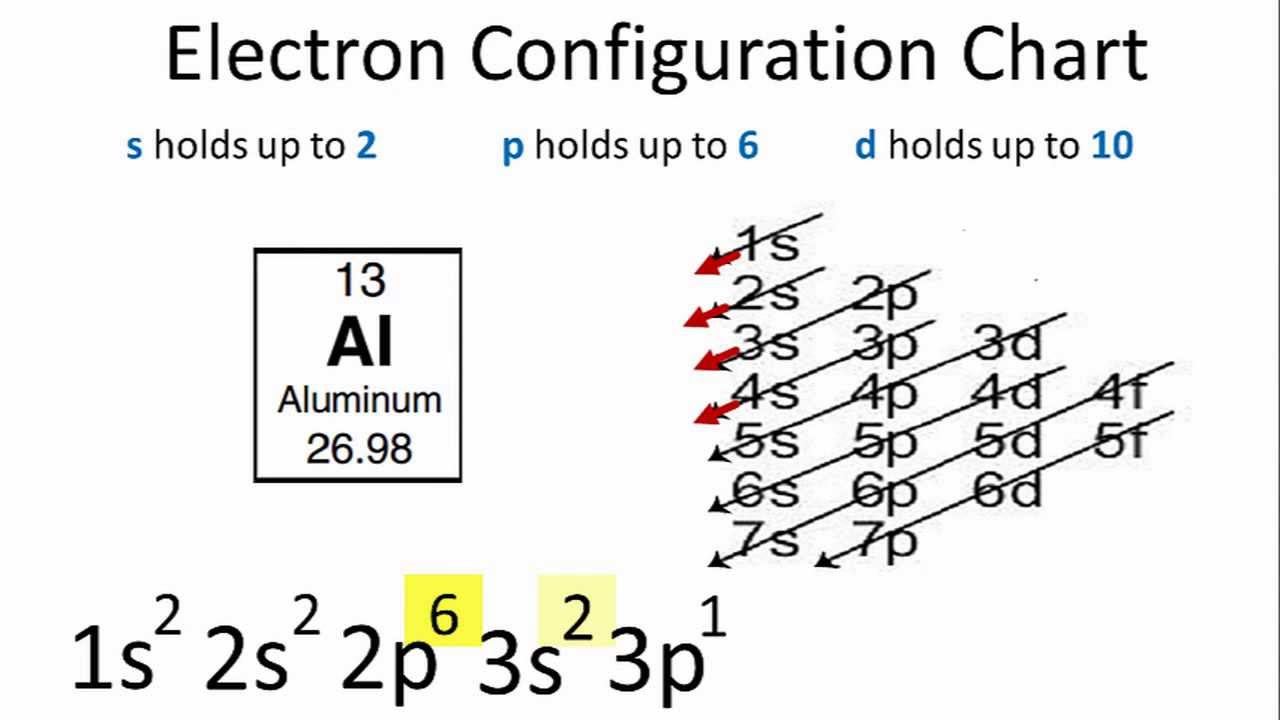
\includegraphics[width=\linewidth]{pic/econfig.jpg}
%
% \end{minipage}%
% \hspace{0.02\linewidth}
% \begin{minipage}[t]{.50\linewidth}
% \vspace{0pt}
%
% \begin{center}
% \begin{tabular}{cccc}
% n & l & m & s\\
% Haupt- & Neben- & Magnet- & Spin- \\
% $1, 2, ...$ & $0, ..., n-1$ & $-l, ..., l$& $\pm \frac{1}{2}$\\
% Schale & Orbital & Orientierung & Spinrichtung\\
% K, L, M, ... & s, p, d, f & x, y z & up/down\\
% \end{tabular}
% \end{center}
% 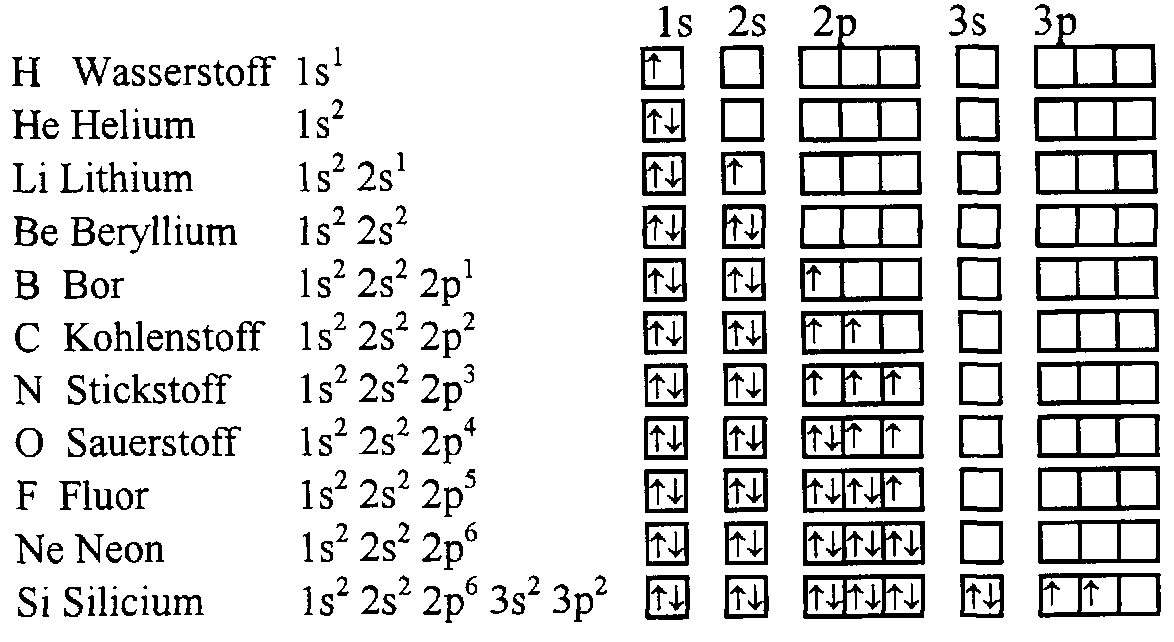
\includegraphics[width=\linewidth]{pic/kaestchen.png}
%
% \end{minipage}
% \end{center}
%
% 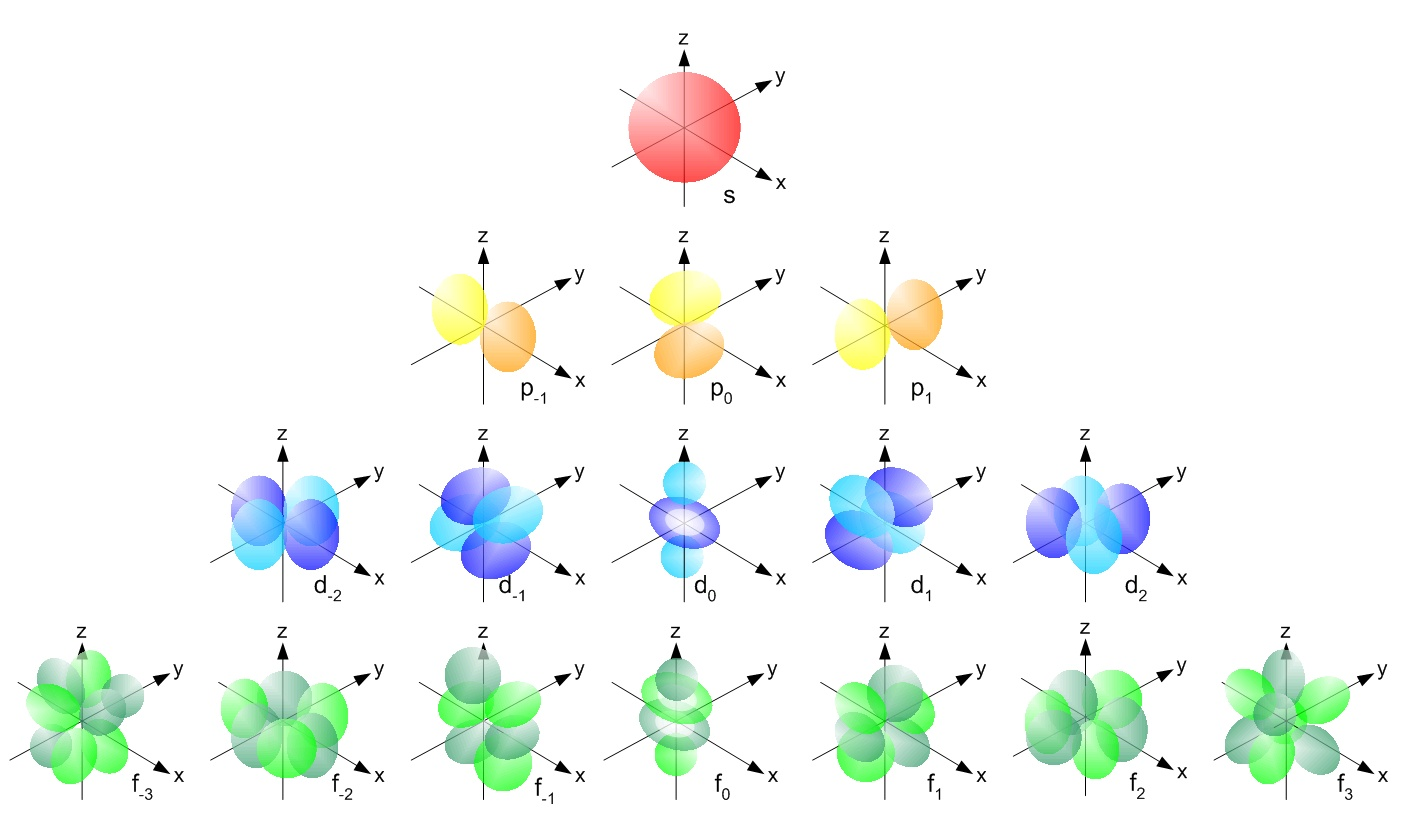
\includegraphics[width=\textwidth]{pic/orbitals.jpg}
%
% \newpage
%
% 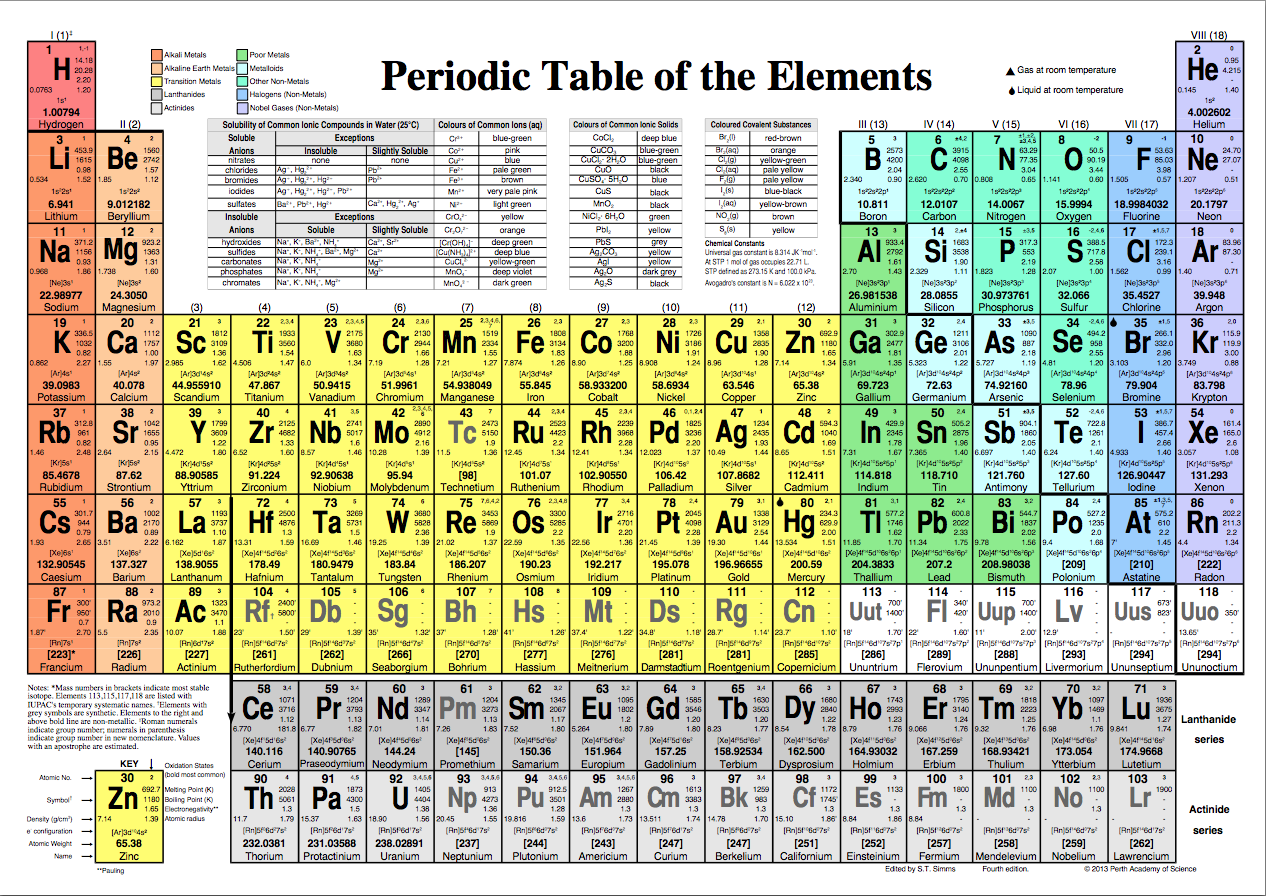
\includegraphics[width=0.9\textheight, angle=90]{pic/pse.png}
% \newpage
%
% \subsection{Stöchiometrie}
%
% \begin{center}
% \begin{minipage}[t]{.45\linewidth}
% \vspace{0pt}
%
% \begin{framed}
% $$m_{Edukte} = m_{Produkte}$$
% \begin{center}
% \textsc{Gesetz von der Erhaltung der Masse}
% \end{center}
% \end{framed}
%
% \begin{framed}
% Elemente in einer chemische Verbindung kommen immer im gleichen konstanten Masseverhältnis vor.
% \begin{center}
% \textsc{Gesetz der konstanten Proportionen}
% \end{center}
% \end{framed}
%
% \begin{framed}
% Die Massenanteile der Elemente in allen chemischen Verbindungen gleicher Elemente stehen in einem ganzzahligen Verhältnis.
% \begin{center}
% \textsc{Gesetz der multiplen Proportionen}
% \end{center}
% \end{framed}
%
% \end{minipage}%
% \hspace{0.02\linewidth}
% \begin{minipage}[t]{.45\linewidth}
% \vspace{0pt}
%
% Molare Masse: $m[g] = n[mol] \cdot M[g/mol]$\\
% $N_A = 6,02217 \cdot 10^{23} =$ N in 12g $^{12}$C\\
% amu: 1u $= 1,6606 \cdot 10^{-24}$g = $\frac{1}{12} m(^{12}$C)\\
% Atommasse: $M = m_A N_A$\\
%
% \begin{tabular}{ll}
% Massenkonz. & $\beta(X)[g/l] = \frac{m(X)[g]}{V[l]}$\\
% Vol.konz. & $\sigma(X)[ml/l] = \frac{V(X)[ml]}{V[l]}$\\
% Stoffmengenkonz. & $c(X)[mol/l] = \frac{n(X)[mol]}{V[l]}$\\
% \end{tabular}
%
% \begin{tabular}{c|c|c}
% Eigenschaft & Periode $\leftrightarrow$ & Gruppe $\updownarrow$\\
% \midrule
% Atomradius & $\uparrow$ & $\downarrow$\\
% Ionisierungsenergie & $\downarrow$ & $\uparrow$\\
% Elektronenaffinität & $\downarrow$ & $\uparrow$\\
% Elektronegativität & $\downarrow$ & $\uparrow$\\
% Metallcharakter & $\downarrow$& $\uparrow$
% \end{tabular}
%
% \end{minipage}
% \end{center}
%
%
% \subsection{Kristalle}
%
% \begin{framed}
% \noindent \textbf{Ionenkristalle}:\\
% \begin{tabular}{l|ccc}
%  & CsCl-Typ & NaCl-Typ & ZnS-Typ\\
% \midrule
% r$^+$/r$^-$ & $> 0,73$ & $0,73 - 0,41$ & $< 0,41$\\
% Koordinationszahl & 8 & 6 & 4\\
% Anordnung & kubisch & oktaedrisch & tetraedrisch
% \end{tabular}
% \end{framed}
% \begin{framed}
% \noindent \textbf{Metallkristalle}:\\
% \begin{tabular}{l|ccc}
%  & Mg-Typ & Cu-Typ & W-Typ\\
% \midrule
% Koordinationszahl & 12 & 12 & 8\\
% Kugelpackung & hexagonal-dicht & kubisch-dicht & kubisch-raumzentriert\\
% Raumausfüllung & 74\% & 74\% & 68\%\\
% Beispiele & Mg, Ti, Co, Zn & Cu, Ni, Al, Ag & W, Na, Cr, Fe
% \end{tabular}
% \end{framed}
%
% \subsection{Chemische Thermodynamik}
%
% \begin{center}
% \begin{minipage}[t]{.5\linewidth}
% \vspace{0pt}
%
% \begin{framed}
% \centering Die Enthalpieänderung ist vom Reaktionsweg unabhängig.
% \begin{center}
% \textsc{Gesetz von Hess}
% \end{center}
% \end{framed}
%
% \begin{tabular}{ll}
% Enthalpie & $\Delta H^{\circ}_{R} = \sum n_{P} \Delta H^{\circ}_{f, P} - \sum n_{E} \Delta H^{\circ}_{f, E}$\\
% Entropie & $\Delta S^{\circ}_{R} = \sum n_{P} \Delta S^{\circ}_{P} - \sum n_{E} \Delta S^{\circ}_{E}$\\
% Freie Energie & $\Delta G^{\circ}_{R} = \sum n_{P} \Delta G^{\circ}_{f, P} - \sum n_{E} \Delta G^{\circ}_{f, E}$
% \end{tabular}
%
% \end{minipage}%
% \hspace{0.02\linewidth}
% \begin{minipage}[t]{.4\linewidth}
% \vspace{0pt}
%
% \begin{framed}
% $$\Delta G = \Delta H - T \Delta S$$
% \begin{center}
% \textsc{Gibbs-Helmholtz-Gleichung}
% \end{center}
% \end{framed}
%
% endotherme Reaktion, $\Delta H > 0$\\
% exotherme Reaktion, $\Delta H < 0$\\
%
% \begin{tabular}{l|cc}
%  & $\Delta H > 0$ & $\Delta H < 0$\\
% \midrule
% $\Delta S > 0$ & spontan bei T$\uparrow$ & immer spontan\\
% $\Delta S < 0$ & nie spontan & spontan T$\downarrow$
% \end{tabular}
%
% \end{minipage}
% \end{center}
%
%
% \subsection{Gasgesetze}
%
% \begin{center}
% \begin{minipage}[t]{.45\linewidth}
% \vspace{0pt}
%
% \begin{framed}
% $$pV = nRT$$
% \begin{center}
% \textsc{Ideale Gasgleichung}
% \end{center}
% \end{framed}
%
% \begin{framed}
% $$V/T = const$$
% \begin{center}
% \textsc{Gesetz von Charles}
% \end{center}
% \end{framed}
%
% \end{minipage}%
% \hspace{0.02\linewidth}
% \begin{minipage}[t]{.45\linewidth}
% \vspace{0pt}
%
% \begin{framed}
% $$p/T = const$$
% \begin{center}
% \textsc{Gesetz von Gay-Lussac}
% \end{center}
% \end{framed}
%
%
% \begin{framed}
% $$n/V = const$$
% \begin{center}
% \textsc{Gesetz von Avogadro}
% \end{center}
% \end{framed}
%
% \end{minipage}
% \end{center}
%
%
%
% \subsection{Lösung}
%
% \begin{center}
% \begin{minipage}[t]{.45\linewidth}
% \vspace{0pt}
%
% \begin{framed}
% $$p = k_H c_l$$
% \begin{center}
% \textsc{Gesetz von Henry}\\
% {\scriptsize $p$: Partialdruck Substanz, $c_l$: Konz. der Lösung}
% \end{center}
% \end{framed}
%
% \end{minipage}%
% \hspace{0.02\linewidth}
% \begin{minipage}[t]{.45\linewidth}
% \vspace{0pt}
%
% \begin{tabular}{l|l}
% Molarität & $\frac{n(X)[mol]}{V(\text{Lösung})[l]}$\\[11pt]
% Molalität & $\frac{n(X)[mol]}{m(\text{Lösungsmittel})[kg]}$\\[11pt]
% Massenprozent & $\frac{m(X)[kg]}{m(\text{Lösung})[kg]} \cdot 100\%$
% \end{tabular}
%
% \end{minipage}
% \end{center}
%
% \subsection{Reaktionskinetik}
%
% \begin{center}
% \begin{minipage}[t]{.45\linewidth}
% \vspace{0pt}
%
% \begin{framed}
% $$K_C = \frac{c_C^{\nu(C)} \cdot c_D^{\nu(D)}}{c_A^{\nu(A)} \cdot c_B^{\nu(B)}}$$
% \begin{center}
% \textsc{Massenwirkungsgesetz}\\
% \scriptsize{(Konzentrationen oder Partialdrücke)}\\
% \scriptsize{für \ch{$\nu$ A + $\nu$ B <=> $\nu$ C + $\nu$ D}}
% \end{center}
% \end{framed}
%
% $K>>1$: Gleichgewicht bei Produkten\\
% $K=1$: Glgw. bei gleicher Konzentration\\
% $K<<1$: Reaktion läuft nicht ab\\
% Reaktionsgeschwindigkeit: $r = \frac{\Delta c}{\Delta t}$
%
% \end{minipage}%
% \hspace{0.02\linewidth}
% \begin{minipage}[t]{.45\linewidth}
% \vspace{0pt}
%
% \begin{framed}
% Übt man auf ein chemisches System im Gleichgewicht einen Zwang aus, so reagiert es so, dass die Wirkung des Zwanges minimal wird.
% \begin{center}
% \textsc{Prinzip von Le Châtelier}
% \end{center}
% \end{framed}
%
% \begin{framed}
% $$K = e^{-\frac{E_A}{RT}}$$
% \begin{center}
% \textsc{Arrhenius-Gleichung}\\
% {\scriptsize $E_A$: Aktivierungsenergie}
% \end{center}
% \end{framed}
%
% \end{minipage}
% \end{center}
%
%
% \subsection{Redox-Reaktionen}
%
% \begin{enumerate}
% \item Reaktionsgleichung aufstellen\\
% $\ch{PbO2 + Mn\pch[2] -> MnO4\mch[] + Pb\pch[2]}$
% \item Oxidationszahlen bestimmen\\
% $\ch{\ox{4,Pb} \ox{-2,O} 2 + \ox{2,Mn} \pch[2] -> \ox{7,Mn} \ox{-2,O} 4\mch[] + \ox{2,Pb} \pch[2]} $
% \item Herausfinden, welche Stoffe reduziert (Ox.zahlen nehmen ab) und welche oxidiert (Ox.zahlen nehmen zu) werden\\
% $\ch{Mn\pch[2]}$ wird oxidiert (von +II auf +VII)\\
% $\ch{PbO2}$ wird reduziert (von +IV auf +II)
% \item Teilreaktionen formulieren\\
% Oxidation: $\ch{"\ox{2,Mn}" \pch[2] -> "\ox{7,Mn}" "\ox{-2,O}" 4\mch[]}$\\
% Reduktion:$ \ch{"\ox{4,Pb}" "\ox{-2,O}" 2 -> "\ox{2,Pb}" \pch[2]}$
% \item Ladungsausgleich\\
% $\ch{"\ox{2,Mn}" \pch[2] -> "\ox{7,Mn}" "\ox{-2,O}" 4\mch[] - 5 e\mch[]}$\\
% $\ch{"\ox{4,Pb}" "\ox{-2,O}" 2 + 2 e\mch[] -> "\ox{2,Pb}" \pch[2]}$
% \item Auf geeignetes Vielfaches bringen und addieren\\
% $\ch{5 PbO2 + 2 Mn\pch[2] -> 2 MnO4\mch[] + 5 Pb\pch[2]}$
% \begin{itemize}
% 	\item Saures Milieu: Auf der Seite mit zu wenig Sauerstoff Wasser addieren, auf der Seite mit zu wenig Wasserstoff Hydronium-Ionen (bzw. \Hpl ) addieren\\
% 	$\ch{5 PbO2 + 2 Mn\pch[2] + 4 \Hpl -> 2 MnO4\mch[] + 5 Pb\pch[2] + 2 H2O}$
% 	\item Basisches Milieu: genauso, aber am Schluss Hydroxid-Ionen (\Hyd) (auf beiden Seiten) addieren, um \Hpl zu neutralisieren.
% \end{itemize}
% \end{enumerate}
%
% \subsection{Elektrochemie}
%
% \begin{center}
% \begin{minipage}[t]{.45\linewidth}
% \vspace{0pt}
%
% \begin{framed}
% $$E = E_0 + \frac{0,059}{n} \log \frac{c(Ox)}{c(Red)}$$
% \begin{center}
% \textsc{Nernst'sche Gleichung}
% \end{center}
% \end{framed}
%
% \end{minipage}%
% \hspace{0.02\linewidth}
% \begin{minipage}[t]{.45\linewidth}
% \vspace{0pt}
%
% \begin{framed}
% $$m = \frac{Mq}{zF}$$
% \begin{center}
% \textsc{1. und 2. Faraday-Gesetz}\\
% \scriptsize{mit F: Faraday-Konstante}
% \end{center}
% \end{framed}
%
% \end{minipage}
% \end{center}
%
% \noindent
% 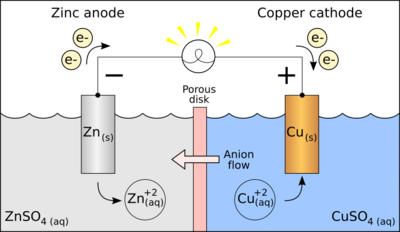
\includegraphics[width=\textwidth]{pic/galva2.png}

\newpage
\section{Konstanten, Abkürzungen, Einheiten und Eselsbrücken}

\subsection{Abkürzungen}

\begin{tabular}{ll}
hO & harmonischer Oszillator\\
sK & starrer Körper\\
CMS & center of mass system\\
iG & ideales Gas\\
bb & schwarzer Körper\\
mP & mathematisches Pendel\\

\end{tabular}

\subsection{Konstanten}
Lichtgeschwindigkeit \dotfill $c = 299 792 458 \frac{m}{s}$\\
Bohr'sches Magneton \dotfill $\mu_B = \frac{e\hbar}{2m_e} = 9,27 \times 10^{-24} J/T = 5,79 \times 10^{-5} eV/T$\\
Vakuumpermeabilität \dotfill $\mu_0 = 4\pi \times 10^{-7} \frac{Vs}{Am}$\\
Gasvolumen bei STP: $V = n V_m$ mit $V_m = 22,4$l/mol\\
$R = 8,314$ J/mol K


\subsection{Eselsbrücken}

$1eV = 8065,541 cm^{-1}$\\
$\hbar c = 197$ eVnm\\
$\lambda = \frac{12{\text \AA}}{\sqrt{U}}$\\
Erdmasse: $6 \cdot 10^{24} kg$\\
$h = 2 \pi \cdot 10^{-34} Js$, $\hbar = 10^{-34} Js$\\
thermische Energie Raumtemperatur: $300K = 25meV$\\
$k_B = \frac{25}{300} \cdot 10^{-3} \frac{eV}{K}$\\
$hc = 1240 eVnm$\\
$m_e = 9,11 \cdot 10^{-31}kg$\\
Sekunden pro Jahr: $\pi \cdot 10^7$\\
$m_p / m_e$: $2000$\\
$1 \frac{km}{s}  = \frac{parsec}{Ma}$\\
$m_p[g] = \frac{1}{N_A} = \frac{1}{6,022 \cdot 10^{23}}$


\subsection{Einheiten}



Drehimpuls: $kg \frac{m^2}{s} = Js$\\
\begin{tabular}{r|l||r|l}
W & $Nm$ & L & $kgm^2$\\
P & $J/s$ & $\varepsilon_0$ & $C^2/Nm^2$\\
$\varphi$ & $J/C$ & $\mu_0$ & $N/A^2$\\
B & $N/Am$ & R & $J/mol K$\\
$\Phi$ & $Tm^2$ & $k_B$ & $J/K$\\
L & $J/A^2$ & $\Gamma$ & $Nm^2/kg^2$\\
I & $W/m^2$ & &
\end{tabular}



\end{document}
